% ==============================================================================
% Modelo para Monografia de Projeto de Graduação - Ciência da Computação (em Português)
% Prof. Vítor E. Silva Souza - NEMO/UFES :: DI/UFES :: PPGI/UFES
% Com adaptações feitas pelo Colegiado de Engenharia de Computação / CT / UFES e pela profª. Monalessa Perini Barcellos (NEMO/UFES).
%
%
% Baseado em abtex2-modelo-trabalho-academico.tex, v-1.9.2 laurocesar
% Copyright 2012-2014 by abnTeX2 group at http://abntex2.googlecode.com/ 
%
% This work may be distributed and/or modified under the conditions of the LaTeX 
% Project Public License, either version 1.3 of this license or (at your option) 
% any later version. The latest version of this license is in
% http://www.latex-project.org/lppl.txt.
%
% IMPORTANTE:
% Instruções encontram-se espalhadas pelo documento. Para facilitar sua leitura,
% tais instruções são precedidas por (*) -- utilize a função localizar do seu
% editor para passar por todas elas.
% ==============================================================================

% Usa o estilo abntex2, configurando detalhes de formatação e hifenização.
\documentclass[
	12pt,				% Tamanho da fonte.
	openright,			% Capítulos começam em página ímpar (insere página vazia caso preciso).
	oneside,			% Para impressão em verso e anverso. Oposto a oneside.
	a4paper,			% Tamanho do papel.
	english,			% Idioma adicional para hifenização.
	french,				% Idioma adicional para hifenização.
	spanish,			% Idioma adicional para hifenização.
	brazil				% O último idioma é o principal do documento.
	]{abntex2}



%%% Importação de pacotes. %%%

% Conserta o erro "No room for a new \count". 
% O comando \reserveinserts deve ser comentado ou não, dependendo da versão do A Utilização do Role-Playing Game (RPG) LaTeX.
\usepackage{etex}
%\reserveinserts{28}

% Usa a fonte Latin Modern.
\usepackage{lmodern}

% Seleção de códigos de fonte.
\usepackage[T1]{fontenc}

% Codificação do documento em Unicode.
\usepackage[utf8]{inputenc}

% Usado pela ficha catalográfica.
\usepackage{lastpage}

% Indenta o primeiro parágrafo de cada seção.
\usepackage{indentfirst}

% Controle das cores.
\usepackage[usenames,dvipsnames]{xcolor}
\usepackage{colortbl} % Para adicionar cor às tabelas
\definecolor{myblue}{cmyk}{86,59,0,40}

\usepackage{pdflscape} % Para girar páginas automaticamente no PDF

% Inclusão de gráficos.
\usepackage{graphicx}

% Tabularx package: melhor controle de leiaute de tabelas.
\usepackage{tabularx}

% Inclusão de páginas em PDF diretamente no documento (para uso nos apêndices).
\usepackage{pdfpages}

% Para melhorias de justificação.
\usepackage{microtype}

% Inclusão de multiplas linhas em uma tabela
\usepackage{multirow}
\usepackage{array}


% Citações padrão ABNT.
\usepackage[brazilian,hyperpageref]{backref}
\usepackage[alf]{abntex2cite}	
\renewcommand{\backrefpagesname}{Citado na(s) página(s):~}		% Usado sem a opção hyperpageref de backref.
\renewcommand{\backref}{}										% Texto padrão antes do número das páginas.
\renewcommand*{\backrefalt}[4]{									% Define os textos da citação.
	\ifcase #1
		Nenhuma citação no texto.
	\or
		Citado na página #2.
	\else
		Citado #1 vezes nas páginas #2.
	\fi}

% \rm is deprecated and should not be used in a LaTeX2e document
% http://tex.stackexchange.com/questions/151897/always-textrm-never-rm-a-counterexample
\renewcommand{\rm}{\textrm}

% Inclusão de símbolos não padrão.
\usepackage{amssymb}
\usepackage{eurosym}

% Para utilizar \eqref para referenciar equações.
\usepackage{amsmath}

% Permite mostrar figuras muito largas em modo paisagem com \begin{sidewaysfigure} ao invés de \begin{figure}.
\usepackage{rotating}

% Permite customizar listas enumeradas/com marcadores.
\usepackage{enumitem}

% Permite inserir hiperlinks com \url{}.
\usepackage{bigfoot}
\usepackage{hyperref}

% Permite usar o comando \hl{} para evidenciar texto com fundo amarelo. Útil para chamar atenção a itens a fazer.
\usepackage{soulutf8}

% Colorinlistoftodos package: to insert colored comments so authors can collaborate on the content.
\usepackage[colorinlistoftodos, textwidth=20mm, textsize=footnotesize]{todonotes}
\newcommand{\aluno}[1]{\todo[author=\textbf{Aluno},color=green!30,caption={},inline]{#1}}
\newcommand{\professor}[1]{\todo[author=\textbf{Professor},color=red!30,caption={},inline]{#1}}

% Permite inserir espaço em branco condicional (incluído no texto final só se necessário) em macros.
\usepackage{xspace}

% Permite incluir listagens de código com o comando \lstinputlisting{}.
\usepackage{listings}
\usepackage{caption}
\DeclareCaptionFont{white}{\color{white}}
\DeclareCaptionFormat{listing}{\colorbox{gray}{\parbox{\textwidth}{#1#2#3}}}
\captionsetup[lstlisting]{format=listing,labelfont=white,textfont=white}
\renewcommand{\lstlistingname}{Listagem}
\definecolor{mygray}{rgb}{0.5,0.5,0.5}
\lstset{
	basicstyle=\scriptsize,
	breaklines=true,
	numbers=left,
	numbersep=5pt,
	numberstyle=\tiny\color{mygray}, 
	rulecolor=\color{black},
	showstringspaces=false,
	tabsize=2,
    inputencoding=utf8,
    extendedchars=true,
    literate=%
    {é}{{\'{e}}}1
    {è}{{\`{e}}}1
    {ê}{{\^{e}}}1
    {ë}{{\¨{e}}}1
    {É}{{\'{E}}}1
    {Ê}{{\^{E}}}1
    {û}{{\^{u}}}1
    {ù}{{\`{u}}}1
    {â}{{\^{a}}}1
    {à}{{\`{a}}}1
    {á}{{\'{a}}}1
    {ã}{{\~{a}}}1
    {Á}{{\'{A}}}1
    {Â}{{\^{A}}}1
    {Ã}{{\~{A}}}1
    {ç}{{\c{c}}}1
    {Ç}{{\c{C}}}1
    {õ}{{\~{o}}}1
    {ó}{{\'{o}}}1
    {ô}{{\^{o}}}1
    {Õ}{{\~{O}}}1
    {Ó}{{\'{O}}}1
    {Ô}{{\^{O}}}1
    {î}{{\^{i}}}1
    {Î}{{\^{I}}}1
    {í}{{\'{i}}}1
    {Í}{{\~{Í}}}1
}



%%% Definição de variáveis. %%%

% (*) Substituir os textos abaixo com as informações apropriadas.
\titulo{Super LabES World: um Role-Playing Game (RPG) para Propósitos Educacionais}
\autor{Israel dos Santos Candeias}
\local{Vitória, ES}
\data{\the\year}
\orientador{Profa. Dra. Patrícia Dockhorn Costa}
% \coorientador{Nome do Co-orientador}
\instituicao{
  Universidade Federal do Espírito Santo -- UFES
  \par
  Centro Tecnológico
  \par
  Colegiado do Curso de Ciência da Computação}
\tipotrabalho{Monografia (PG)}

% Preâmbulo (tipo do trabalho, objetivo, nome da instituição, área de concentração, etc.).
\preambulo{Monografia apresentada ao Curso de Ciência da Computação do Centro Tecnológico da Universidade Federal do Espírito Santo, como requisito parcial para obtenção do Grau de Bacharel em Ciência da Computação.}

% Macros específicas do trabalho.
% (*) Inclua aqui termos que são utilizados muitas vezes e que demandam formatação especial.
% Os exemplos abaixo incluem i* (substituindo o asterisco por uma estrela) e Java com TM em superscript.
% Use sempre \xspace para que o LaTeX inclua espaço em branco após a macro somente quando necessário.
\newcommand{\istar}{\textit{i}$^\star$\xspace}
\newcommand{\java}{Java\texttrademark\xspace}
\newcommand{\latex}{\LaTeX\xspace}




%%% Configurações finais de aparência. %%%

% Altera o aspecto da cor azul.
\definecolor{blue}{RGB}{41,5,195}

% Informações do PDF.
\makeatletter
\hypersetup{
	pdftitle={\@title}, 
	pdfauthor={\@author},
	pdfsubject={\imprimirpreambulo},
	pdfcreator={LaTeX with abnTeX2},
	pdfkeywords={abnt}{latex}{abntex}{abntex2}{trabalho acadêmico}, 
	colorlinks=true,				% Colore os links (ao invés de usar caixas).
	linkcolor=blue,					% Cor dos links.
	citecolor=blue,					% Cor dos links na bibliografia.
	filecolor=magenta,				% Cor dos links de arquivo.
	urlcolor=blue,					% Cor das URLs.
	bookmarksdepth=4
}
\makeatother

% Espaçamentos entre linhas e parágrafos.
\setlength{\parindent}{1.3cm}
\setlength{\parskip}{0.2cm}



%%% Páginas iniciais do documento: capa, folha de rosto, ficha, resumo, tabelas, etc. %%%

% Compila o índice.
\makeindex

% Inicia o documento.
\begin{document}

% Brasão da instituição.
\begin{figure}
	\centering
	
\includegraphics[width=.20\textwidth]{figuras/brasao.jpg} 
	\label{fig-brasao}
\end{figure}

\begin{center}
	\textbf{\textsf{UNIVERSIDADE FEDERAL DO ESPÍRITO SANTO}}
	
	\textbf{\textsf{CENTRO TECNOLÓGICO}}
	
	\textbf{\textsf{COLEGIADO DO CURSO DE CIÊNCIA DA COMPUTAÇÃO}}
	
	\large{\textbf{\textsf{  }}}
	
	\large{\textbf{\textsf{  }}}
\end{center}

% Retira espaço extra obsoleto entre as frases.
\frenchspacing

% Capa do trabalho.
\imprimircapa

% Folha de rosto (o * indica que haverá a ficha bibliográfica).
\imprimirfolhaderosto*


% Ficha catalográfica.
% (*) Escolher entre as versões de ficha catalográfica abaixo (comente aquela que não quiser usar).

% Versão 1: caso a biblioteca da sua universidade lhe forneça um PDF (adequar o nome do arquivo).
% \begin{fichacatalografica}
%     \includepdf{include-fichacatalografica.pdf}
% \end{fichacatalografica}

% Versão 2: caso você tenha que inserir sua própria ficha catalográfica.
% (*) Neste caso, preencher palavras-chave e adicione co-orientador (se houver).
\begin{fichacatalografica}
	\vspace*{\fill}
	\hrule
	\begin{center}
	\begin{minipage}[c]{12.5cm}
	
	\imprimirautor
	
	\hspace{0.5cm} \imprimirtitulo  / \imprimirautor. --
	\imprimirlocal, \imprimirdata-
	
	\hspace{0.5cm} \pageref{LastPage} p. : il. (algumas color.) ; 30 cm.\\
	
	\hspace{0.5cm} \imprimirorientadorRotulo~\imprimirorientador\\
	
	\hspace{0.5cm}
	\parbox[t]{\textwidth}{\imprimirtipotrabalho~--~\imprimirinstituicao,
	\imprimirdata.}\\
	
	\hspace{0.5cm}
		1. Palavra-chave1.
		2. Palavra-chave2.
		I. Souza, Vítor Estêvão Silva.
		II. Universidade Federal do Espírito Santo.
		IV. \imprimirtitulo \\ 			
	
	\hspace{8.75cm} CDU 02:141:005.7\\
	
	\end{minipage}
	\end{center}
	\hrule
\end{fichacatalografica}


% Folha de aprovação.
% (*) Escolher entre as versões de ficha catalográfica abaixo (comente aquela que não quiser usar).

% Versão 1: cópia digitalizada da folha de aprovação assinada pela banca.
% \includepdf{include-folhadeaprovacao.pdf}

% Versão 2: folha de aprovação em branco.
% (*) Ajustar a data e os nomes dos participantes da banca.
\begin{folhadeaprovacao}
  \begin{center}
    {\ABNTEXchapterfont\large\imprimirautor}
    \vspace*{\fill}\vspace*{\fill}
    \begin{center}
      \ABNTEXchapterfont\bfseries\Large\imprimirtitulo
    \end{center}
    \vspace*{\fill}
    \hspace{.45\textwidth}
    \begin{minipage}{.5\textwidth}
        \imprimirpreambulo
    \end{minipage}%
    \vspace*{\fill}
   \end{center}
   Trabalho aprovado. \imprimirlocal, (dia) de (mês) de (ano):
   \assinatura{\textbf{\imprimirorientador} \\ Orientador} 
   \assinatura{\textbf{Nome do Membro da Banca} \\ Nome da Instituição}
   \assinatura{\textbf{Nome do Membro da Banca} \\ Nome da Instituição}
   %\assinatura{\textbf{Nome do Membro da Banca} \\ Nome da Instituição}
   %\assinatura{\textbf{Nome do Membro da Banca} \\ Nome da Instituição}
   \begin{center}
    \vspace*{0.5cm}
    {\large\imprimirlocal}
    \par
    {\large\imprimirdata}
    \vspace*{1cm}
  \end{center}  
\end{folhadeaprovacao}


% Dedicatória.
% (*) Escrever dedicatória ou remover/comentar seção.
\begin{dedicatoria}
   \vspace*{\fill}
   \centering
   \noindent
   \textit{Lorem ipsum dolor sit amet, consectetur adipiscing elit. Duis malesuada laoreet leo at interdum. Nullam neque eros, dignissim sed ipsum sed, sagittis laoreet nisi.} \vspace*{\fill}
\end{dedicatoria}


% Agradecimentos.
% (*) Escrever agradecimentos ou remover/comentar seção.
\begin{agradecimentos}

\end{agradecimentos}


% Epígrafe.
% (*) Escrever epígrafe ou remover/comentar seção.
\begin{epigrafe}
    \vspace*{\fill}
	\begin{flushright}
		\textit{``Lorem ipsum dolor sit amet, consectetur adipiscing elit. \\
		Duis malesuada laoreet leo at interdum. Nullam neque eros, dignissim \\
		sed ipsum sed, sagittis laoreet nisi.\\
		(Lipsum generator)}
	\end{flushright}
\end{epigrafe}


% Resumo em português.
% (*) Escrever resumo e palavras-chave.
\setlength{\absparsep}{18pt}
\begin{resumo}

\textbf{Palavras-chaves}: lorem. ipsum. dolor. sit. amet.
\end{resumo}

% Insere lista de ilustrações.
\pdfbookmark[0]{\listfigurename}{lof}
\listoffigures*
\cleardoublepage

% Insere lista de tabelas.
\pdfbookmark[0]{\listtablename}{lot}
\listoftables*
\cleardoublepage

% Lista de abreviaturas e siglas.
% (*) Preencher com as siglas usadas ao longo do texto e seus significados.
\begin{siglas}
  \item[UML] Unified Modeling Language
\end{siglas}

% Insere o sumário.
\pdfbookmark[0]{\contentsname}{toc}
\tableofcontents*
\cleardoublepage



%%% Início da parte de conteúdo do documento. %%%

% Marca o início dos elementos textuais.
\textual

% Inclusão dos capítulos.
% (*) Para facilitar a organização, os capítulos foram divididos em arquivo separados e colocados dentro da.
% pasta capitulos/. Caso o aluno prefira trabalhar com um só arquivo, basta substituir os comandos \include 
% pelos conteúdos dos arquivos que estão sendo incluídos, excluindo a pasta capitulos/ em seguida.
% ==============================================================================
% PG - Nome do Aluno
% Capítulo 1 - Introdução
% ==============================================================================
\chapter{Introdução}
\label{sec-intro}
% Talvez, devemos fazer da seguinte forma: falar das dificuldades do lab (no embarque, com o aprendizado, etc...), depois falar sobre as possibilidades de jogos como ferramenta para auxiliar no aprendizado
O Laboratório de Práticas em Engenharia de Software “Ricardo de Almeida Falbo” LabES \footnote{Laboratório de Práticas em Engenharia de Software – LabES \url{https://labes.inf.ufes.br}.}
 é um importante laboratório de extensão vinculado ao  Departamento de Informática do Centro Tecnológico da UFES. Seu objetivo é capacitar estudantes a aplicar métodos, técnicas e procedimentos de ponta em Engenharia de Software, visando aproximar sua formação às necessidades dos diversos setores produtivos, além de produzir software a partir de demandas de clientes internos e externos à Universidade \cite{LabES}. Atualmente, o LabES integra cinco projetos ativos, sendo eles:
\begin{itemize}
	\item FAVO: O FAVO tem como objetivo o desenvolvimento de um aplicativo para fomentar a cultura de inovação nas organizações, onde os usuários podem acompanhar as ações de inovação e participar de programas de ideias de forma ``gamificada'';
	
	\item Hub Criativo Virtual: Também simplesmente chamado Hub ES+ visa a construção de um \textit{Hub} Criativo Virtual, plataforma online que conectará os espaços físicos do Hub ES+ com o mundo virtual, utilizando recursos de \textit{gamificação} para prover um ambiente imersivo para interação e formação dos criativos e integrando também um painel de dados com as pesquisas do Observatório da Economia Criativa Capixaba e o portal Vitrine Criativa da SECULT-ES;
	
	\item Marvin: Tem como objetivo atender solicitações específicas da graduação e pós-graduação do Departamento de Informática da UFES, por exemplo, problemas relacionados a tarefas administrativas vinculadas aos cursos, departamentos e programas da UFES; sendo assim, esse projeto visa a integração das ferramentas existentes e o desenvolvimento de novas ferramentas não cobertas pelos atuais sistemas de informação do NTI/UFES;
	
	\item SEEDES: Trata-se do primeiro programa público de aceleração de \textit{startups} no Espírito Santo, um programa do Governo do Estado do Espírito Santo que tem por objetivo fomentar o desenvolvimento de empresas e ideias inovadoras. No LabES, o projeto SEEDES se propõe a desenvolver uma plataforma Web pública para o Ecossistema Capixaba de Inovação com coleta de dados e indicadores sistemáticos do ecossistema local, visando viabilizar um painel com busca automatizada com supervisão na plataforma;
	
	\item SigAMAES: Projeto ao qual este graduando participou. Esse projeto tem como objetivo o desenvolvimento e manutenção de um sistema de informação gerencial que serve de apoio às atividades exercidas pela instituição Associação dos Amigos dos Autistas do Espírito Santo (AMAES)\footnote{AMAES – Associação dos Amigos dos Autistas do Estado do Espírito Santo \url{https://amaes.org.br}.}, uma instituição sem fins lucrativos, oficialmente constituída em 2001 por pais de autistas e também administrada voluntariamente por eles além de familiares e amigos dos autistas; o sistema tem como principais funcionalidades facilitar o cadastro de informações sobre os autistas, prover mecanismos para gerenciamento dos atendimentos oferecidos pela instituição, oferecer controle de acesso a informações sensíveis e produzir análises estatísticas sobre os dados coletados.
\end{itemize}
Atualmente, o embarque de novos membros estudantes no laboratório começa pelo preenchimento de um formulário no site oficial que vai para um cadastro de reserva que, além das informações pessoais e outras informações sobre disponibilidade, há duas perguntas que dão uma ideia sobre o nível técnico do estudante. Caso o estudante ainda não tenha conversado com algum professor sobre um projeto específico, com as informações do cadastro, cabe aos professores responsáveis pelo laboratório decidir em qual dos atuais cinco projetos do laboratório o estudante será alocado.  Embora essa abordagem seja eficaz para avaliar o interesse do estudante no laboratório, ela apresenta limitações, como: (i) entender o nível de conhecimento técnico do estudante; (ii) fornecer ao estudante informações importantes sobre o laboratório.


%%% Início de seção. %%%
\section{Motivação e Justificativa}
\label{sec-intro-motjus}
Somando-se às considerações acima, uma caraterística de alguns projetos do LabES é a alta rotatividade da equipe, devido à dificuldade em oferecer bolsas de estudos para todos os estudantes membros. Esse fenômeno gera atrasos no desenvolvimento dos projetos, uma vez que novos membros precisam passar por etapas de treinamentos para que consigam começar a produzir. Quando passam algum tempo no projeto e tornam-se mais experientes e capazes de produzir e ajudar novos membros, os estudantes deixam o projeto, em busca de estágios remunerados. Ou seja, há uma grande dificuldade de manter membros \textit{seniors} nas equipes, que possam ajudar no embarque de novos estudantes. 

Diante desse cenário, surge uma necessidade de ajudar esses novos estudantes no seu aprendizado inicial, pavimentando a entrada de novos alunos a fim de acelerar o progresso dos alunos para que sejam capazes de contribuir nos projetos do laboratório.
%há um gap muito grande aqui. Estamos falando de labes, embarque, dificuldades dos projetos do labes... de repente vem algo sobre jogos! Temos que preencher esse gap. Talvez falar algo específico sobre como ajudar no aprendizado com gamificação? Tem que pensar um pouco melhor...

Com os avanços da tecnologia e consequentemente da qualidade de vida, a busca por entretenimento é cada vez mais presente. Mediante o uso frequente de celulares e computadores, as constantes notificações distraem os estudantes, comprometendo seus resultados. Cada vez mais, os professores e pedagogos têm se reinventado, criando novas estratégias em suas aulas para conseguirem transmitir seu conteúdo de forma eficaz. Por isso, gradativamente, tem-se usado mais tecnologia para ensinar, e uma das abordagens comumente utilizadas é o uso de jogos. 

Os jogos apresentam-se como um recurso útil na educação, pois aumentam o interesse dos estudantes nos conteúdos abordados. Um exemplo disso é a \textit{“Quest to Learn}” (Q2L)\footnote{\textit{“Quest to Learn}” (Q2L) \url{https://q2l.org}} uma escola pública de Nova York nos Estados Unidos que, diferentemente das escolas tradicionais, todo o seu currículo é baseado nos princípios de design de jogos. Seus resultados de proficiência disciplinar mostraram-se superiores às demais escolas da mesma região, com destaque em relação à leitura; 27\% a mais \cite{Q2L}.

O Brasil é o décimo maior mercado de games do mundo, com mais de 100 milhões de jogadores. Em sua última pesquisa, a PGB (Pesquisa Game Brasil) apontou que 73,9\% dos brasileiros tem o hábito de jogar video-games \cite{PGB}. Além disso, a indústria brasileira de games ainda é muito pequena, existem apenas 1.042 estúdios de desenvolvimento de games ativos em todo país que, se somados, possuem um faturamento estimado de US\$ 252,6 milhões \cite{Abragames}, um pouco menos que 10\% de todo o faturamento da indústria de games mundial no mesmo ano, apontando a necessidade de fomentação do desenvolvimento de jogos locais.

%esse trabalho também pode ser usado como material de apoio a programadores e entusiastas interessados em desenvolvimento de jogos. como o Brasil tem um mercado em potencial nessa industria que movimenta Bilhões,% 

% Outra informação relevante é que segundo a principal plataforma de dados de jogos para PC e console  Newzoo, o Brasil é o décimo maior mercado de games do mundo, com mais de 100 milhões de jogadores que gastaram 2,7 bilhões de dólares em somente em 2022 \cite{NEWZOO}, a PGB (Pesquisa Game Brasil) apontou em sua ultima pesquisa que 73,9\% das pessoas afirmaram ter o hábito de jogar videogames, sendo que 85,4\% destes afirmam ter essa como sua principal fonte de entretenimento \cite{PGB} . Vendo que é uma área atraente aos publico, surgiu a ideia de criar um jogo com propósito educativo,  um game que pudesse  direcionar o aprendizado.


%%% (Associação Brasileira das Desenvolvedoras de Games) divulgado em 2023  %%%

% existem muitos temas a serem explorados, muitos jogos a serem produzidos


% de simulação RPG (Role-playing game) ou simplesmente "jogo de interpretação de papéis",  em português , onde o jogador assume o papel de um estudante que tem o objetivo de entrar no LabES, e assim a história vai levando o estudante a alguns desafios e enquanto direciona o conhecimento forma lúdica sobre aspectos que são consideradas de base para um aluno entrar com o pé direito no projeto.


%%% Início de seção. %%%
\section{Objetivos}
\label{sec-intro-obj}

% Nesta subseção, deve ser descrito o objetivo geral do trabalho, detalhando em seguida, seus objetivos específicos. O \textbf{Objetivo Geral} expressa a finalidade principal do trabalho: para quê? Deve ter coerência direta com o tema do trabalho e ser apresentado em uma frase que inicie com um verbo no infinitivo. O objetivo geral do trabalho está relacionado ao resultado principal do trabalho. Os \textbf{Objetivos Específicos} apresentam os detalhes ou desdobramentos do objetivo geral que levam a resultados intermediários e relevantes para alcançar o objetivo geral. Sempre será mais de um objetivo específico, todos iniciando com verbo no infinitivo.

O Objetivo principal deste projeto de graduação é desenvolver um jogo capaz de apoiar o embarque de novos membros do LabES; este jogo deve: (i) ser um jogo introdutório que aborda questões básicas e úteis para o começo de seu tempo de colaboração no laboratório; (ii) ter um \textit{feedback} ativo e eficaz, ou seja, ao errar, a mecânica proposta deve informar o jogador de forma imediata, garantindo um aprendizado acelerado; (iii) direcionar o jogador para materiais acadêmicos que ensinem de forma organizada e eficiente o que o estudante ainda não tenha aprendido. Estas características tornarão o jogo não apenas capaz de testar o nível do aluno, mas também elevá-lo.

    São objetivos específicos deste trabalho:
\begin{itemize}
    \item Projetar o sistema;
    \item Realizar o levantamento de requisitos do sistema;
    \item Definir as tecnologias a serem utilizadas;
    \item Desenvolver as questões a serem testadas/ensinadas;
    \item Estruturar um protótipo;
    \item Desenvolver o jogo;
\end{itemize}

%diferentemente de uma prova formal, onde toda essa parte ocorre de forma muito mais lenta, desgastante e trabalhosa para ambas as partes.%


% onde de forma divertida o estudante acaba adquirindo conhecimentos e tendo um direcionamento do seu aprendizado tendo acesso a materiais de estudo que são considerados importantes para começar sua caminhada no LabES e assim começar com o pé direito maximizando a sua curva de aprendizado

% Além disso essa monografia pode ser usada como material de apoio a programadores e entusiastas que gostariam de iniciar no pygame e desenvolvimento de jogos, uma vez que o conteúdo em português sobre game design é ainda escasso. Mais a frente teremos um capítulo dedicado a explicar como e quais ferramentas foram utilizadas no desenvolvimento desse jogo 
% \#\#\# Acrescentar mais aqui depois

% esse trabalho também tem por objetivo ser um material de apoio a programadores e entusiastas interessados em desenvolvimento de jogos.


%%% Início de seção. %%%
\section{Método de Desenvolvimento do Trabalho}
\label{sec-intro-met}
%%%Nesta subseção, deve ser apresentado o \textbf{Método de Desenvolvimento} (ou o \textbf{Método de Pesquisa}, quando for o caso) utilizado no trabalho. Aqui são apresentadas as atividades realizadas e os procedimentos/técnicas que foram usados durante o desenvolvimento do trabalho.%%%
O Desenvolvimento do trabalho começou com a busca de uma resposta fundamental: ``Como fazer um jogo educativo ser divertido?''. Este é um dos maiores desafios relacionados aos jogos educativos: torná-los interessantes de forma que o jogador seja incentivado a continuar jogando e, consequentemente, aprendendo. Com essa resposta em mãos, foi realizado um levantamento das principais funcionalidades e mecânicas que o jogo deveria contemplar.

O próximo passo foi a realização de uma pesquisa de \textit{engines}, bibliotecas e ferramentas gerais que seriam utilizadas no desenvolvimento do jogo. Nessa pesquisa foram feitas análises da capacidade de cada ferramenta em reproduzir as funcionalidades definidas na etapa anterior. Após a definição do diferencial do jogo e das ferramentas a serem utilizadas em sua implementação, iniciou-se a etapa de desenvolvimento.

No início do projeto, o escopo do jogo não estava plenamente definido, por isso o andamento do desenvolvimento foi feito com base no modelo evolucionário em espiral, onde novos requisitos são adquiridos em paralelo à evolução do sistema. Dessa forma, a cada nova versão do jogo eram feitas reuniões com a orientadora e com colegas de curso, onde surgiam novas ideias e melhorias.

Na última etapa do projeto, com o jogo já implementado, foi realizada a sua disponibilização aos membros do laboratório, membros egressos. Após o teste do jogo, eles eram orientados a preencher um formulário para coletar informações de mecânica e usabilidade do jogo. Estes resultados foram aproveitados na geração das conclusões do projeto, que puderam quantificar seu impacto em um ambiente mais próximo ao real.




%%% Início de seção. %%%
\section{Organização da Monografia}
\label{sec-intro-organizacao}
%%% Além desta introdução, este modelo de monografia é composto por outros cinco capítulos: %%%

Este trabalho está dividido em seis capítulos contando com este, apresentados na seguinte ordem:


\begin{itemize}
	\item O Capítulo~\ref{sec-referencial} apresenta uma fundamentação teórica dos conceitos e tecnologias
 utilizados no trabalho;
	
	\item O Capítulo~\ref{sec-contribuicao} apresenta o escopo do projeto e a análise de requisitos do jogo;

        \item O Capítulo \ref{sec-implementacao} apresenta detalhes da implementação e também as decisões da aplicação;
        
	\item O Capítulo~\ref{sec-avaliacao} apresenta a apresentação e avaliação da proposta;
	
	\item O Capítulo~\ref{sec-conclusoes} apresenta as considerações finais do trabalho;
	
\end{itemize}



% ==============================================================================
% PG - Israel dos Santos Candeias
% Capítulo 2 - Referencial Teórico
% ====================================== 2.0 ================================
\chapter{Referencial Teórico e Tecnologias Utilizadas}
\label{sec-referencial}
% Este capítulo deve apresentar os aspectos relativos ao conteúdo teórico relevante para o trabalho.  Incluirá conhecimento adquirido a partir de livros, artigos, relatórios técnicos, dissertações, teses e outros materiais bibliográficos.  O capítulo deve apresentar, além do referencial teórico, informações sobre as tecnologias utilizadas no trabalho. O capítulo deve ter cerca de 12-15 páginas e deve demonstrar conhecimento básico da literatura técnico-científica sobre o tema abordado no trabalho.
Neste capítulo serão apresentados os conceitos teóricos que guiaram o desenvolvimento do jogo, bem como as tecnologias usadas para implementar o sistema, no capítulo \ref{sec-principios-de-design-de-software} abordamos alguns dos conceitos fundamentais de engenharia de software e também como isso foi usado nessa trabalho, na seção \ref{sec-desenvolvimento-de-jogos} é exposto alguns princípios básicos de desenvolvimento de jogos e as ferramentas e padrões que foram utilizadas na programação, a seção \ref{sec-mapas} fala sobre os programas que foram utilizados para o desenvolvimento de mapas desse jogo e a seção \ref{sec:pixel-art} explica como a parte artística do jogo foi feita e brevemente a ferramenta que foi utilizada.
% colocar os links para as seções explicando oq cada uma fala 

% =============================== 2.1 Princípios de Design de Software ===========================
\section{Princípios de Design de Software}
\label{sec-principios-de-design-de-software}
Os princípios de design de software constituem diretrizes fundamentais para o desenvolvimento de sistemas de software eficazes, robustos e manuteníveis. Esses princípios orientam todo o ciclo de vida do software desde o surgimento da ideia até o sistema em produção. 
\subsection{Engenharia de Software}
\label{sec:engenharia-de-software}
A engenharia de software é a área da computação que se preocupa em propor e aplicar princípios de engenharia na construção de softwares\cite{engsoftmoderna} ou seja é uma área de estudos da computação que se preocupa em projetar, arquitetar melhorar a qualidade dos produtos de software aumentando assim a produtividade no processo de desenvolvimento. 

Para seguir as práticas recomendadas de engenharia de software o primeiro passo a ser definido é qual paradigmas de processo de software ser seguido, existem vários modelos para diferentes cenários possíveis, o escolhido para esse trabalho foi o modelo evolutivo.

O modelo evolutivo como o próprio nome sugere, os requisitos vão evoluindo conforme a aplicação evolui, esse processo ocorre em paralelo à evolução da aplicação, esse paradigma é muito útil quando o cliente não tem todas as funcionalidades necessárias para a solução. Nesse contexto foi oque mais se adequou a esse trabalho tendo em vista que nem todos os requisitos eram bem definidos de início e as funcionalidades do jogo precisam ser validadas frequentemente, uma vez que, a jogabilidade precisa ser atraente ao público, então a cada nova versão foram realizadas reuniões com colegas, e com a orientadora, a fim de receber feedbacks que auxiliem na melhoria dos recursos de modo contínuo.

A Figura \ref{spiral-model} ilustra esse modelo

\newpage
\begin{figure}
    \centering
    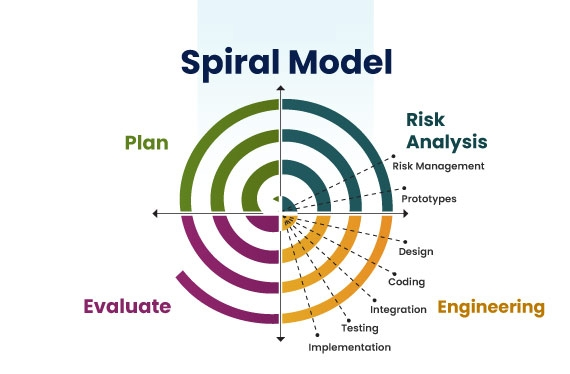
\includegraphics[width=0.9\linewidth]{figuras/spiral-model.jpg}
    \caption{Ciclo de vida do modelo espiral}
    \label{spiral-model}
\end{figure}
Cada uma das atividades realizadas no modelo ilustrado acima são:
\begin{itemize}
    \item \textbf{Planejamento:} A fase de planejamento é base sobre a qual todo o projeto de desenvolvimento de software deve ser construído. Durante essa fase foram definidos os requisitos e as ferramentas que seriam utilizadas;
    \item \textbf{Análise de riscos:} Nessa fase é feito tanto o levantamento dos riscos associados ao desenvolvimento do sistema, mas também como mitigá-los no geral sendo uma etapa para gerenciar os riscos, e na avaliação da viabilidade técnica;
    \item \textbf{Engenharia (Projeto e Codificação):} Aqui é onde são desenvolvidos os o designs do software, codificação, integração, testes e por fim a implantação no sistema;
    \item \textbf{Validação:} Ao chegar nessa fase já temos uma versão inicial do projeto, agora podemos coletar feedbacks o observações sobre o sistema, essa etapa é fundamental nessa abordagem, pois a qualidade da próxima versão é diretamente proporcional a qualidade dos feedbacks aqui coletados;
\end{itemize}

Essas Etapas se repetem num \textit{loop}, o número exato de \textit{loops} do modelo é indefinido e varia de projeto para projeto. Cada loop da espiral é nomeado fase do processo de desenvolvimento de software.

\section{RPG}
\label{sec:rpg}
\subsection{RPG de Mesa}
\label{sec:rpg-de-mesa}
Em meados de 1974 nos Estados Unidos foi publicado o um jogo chamado \textit{Dungeons} \& \textit{Dragons} \footnote{D\&D - \textit{Dungeons and Dragons} \url{https://dnd.wizards.com/pt-BR}}, esse que e considerado o primeiro RPG (\textit{Role-Playing Game}) em português jogo de interpretação de papéis com ambientação em um universo de fantasia medieval.

A ideia do jogo consistem em cada jogador na mesa construir a história, personalidade e ficha de seu personagem, após isso o mestre de jogo ou narrador que já planejou a história anteriormente irá dar prosseguimento narrando a história dando início do jogo, conduzido pela imaginação. Os jogadores jogam dados para determinar quais dos seus ataques acertam ou erram e se seu personagem percebe ou não uma armadilha escondida, todas as ações são determinadas através dos dados. 

A ficha de personagem é um documento que deve conter todas as características que definem os detalhes necessários do seu personagem. É ela que diz o quão bom seu personagem é em fazer em determinadas ações, já a história se refere a um plano de fundo que o jogador inventa para o seu personagem com o intuito de contribuir para um jogo rico em detalhes. 

\subsection{RPG Eletrônico}
\label{sec:rpg-eletronico}
Após o sucesso do RPG de mesa, e com o avanço da tecnologia esse estilo de jogo saiu da mesa e chegou aos computadores e consoles já não mais precisando depender totalmente da imaginação, os computadores renderizam gráficos cada vez mais melhores e realistas. Esse estilo de jogo se popularizou e atualmente é um dos gêneros de jogos mais populares segundo a NEWZOO \cite{NEWZOO}.

Atualmente todos os RPGs giram em torno de um universo fictício chamado ambientação que pode ser medieval, ocidental, espacial, realístico e o que mais a imaginação inventar. Esse universo forma o cenário onde os personagens interagem e constroem a sua história, profissão, cultura e tecnologias. \cite{duflo1999jogo}

\subsection{O RPG na Educação}
\label{sec:rpg-na-educacao}
Esse gênero têm se destacado não apenas no video-game, mas também como ferramentas versáteis com aplicações em diversas áreas. Esses jogos, caracterizados pela imersão em narrativas interativas e pela personalização de personagens já foram utilizados em diversas áreas fora o entretenimento e tiveram resultados bem positivos. Na UFG (universidade de Goiás) foi desenvolvido um jogo RPG cujo para o curso de Ciências e Biologia, o 
objetivo era mediar a aprendizagem, diversificar e avaliar a transmissão do conhecimento e que fosse útil em sua prática profissional. O jogo consistia de uma aventura dentro do corpo humano com 25 questões a respeito de Fisiologia Humana Básica, os alunos do curso demonstraram grande interesse pelo jogo e aprovaram o modelo didático e perceberam sua eficácia ao associar a imaginação e a forma como pode ser utilizado para ensinar e avaliar os conhecimentos adquiridos.\cite{soares2016role}


%  ================================ 2.2 Princípios de Game Design ================================
% 

% =================== PYGAME-CE =======================================
\section{Desenvolvimento de Jogos}
\label{sec-desenvolvimento-de-jogos}
Um jogo é um tipo de aplicativo que normalmente é usado para fins de entretenimento, mas também pode ser projetado para objetivos mais sérios, com potencial de aplicação em diversas áreas, como exemplo educação, negócios e saúde.
Desenvolver um jogo é uma tarefa desafiadora devido às diversas atividades multidisciplinares envolvidas, tornando o processo altamente complexo. 

\subsection{Princípios de Game Design}
\label{sec:principios-de-game-design}
O processo de aprendizagem envolvido na criação e no desenvolvimento de jogos integra uma ampla variedade de conhecimentos. Para criar um jogo, é fundamental dominar não apenas a programação, mas também áreas como Música, Desenho, inglês, Geometria, Física, Matemática, Lógica, Geografia e Linguagens se tornam indispensáveis, pois o desenvolvimento de um jogo exige o domínio de programação, design gráfico, efeitos sonoros, criação de fases (\textit{level design}), elaboração de histórias e narrativas (\textit{storytelling}), temática e contextualização.

Nos primeiros dias do desenvolvimento de videogames, os jogos eram criados por grupos pequenos de pessoas, porém, com a complexidade dos jogos aumentando e a industria vendo oportunidades sérias, as equipes eventualmente foram acompanhando o ritmo a especialização está se tornando cada vez mais necessária à medida que os jogos se tornam maiores uma equipe de produção média inclui vários membros. Atualmente, uma equipe de desenvolvimento de jogos engloba profissionais multidisciplinares de diversas áreas, cada um com um foco especifico para a produção do jogo. Scott Rogers cita em seu livro \cite{GameDesign} as seguintes: 
\begin{itemize}
    \item \textbf{Programador(a):} Responsável pela programação do software do jogo e das ferramentas utilizadas quando se aplicam também escreve o documento técnico;
    \item \textbf{Artista:} Responsável pela representação visual dos componentes do jogo desde as interfaces aos personagens estipulados no documento técnico ;
    \item \textbf{Designer do Jogo:} cria as ideias e regras que compõem o jogo do conceito até a forma final também cuida da documentação do sistema de interação;
    \item \textbf{Produtor(a): }Responsável por supervisionar toda a equipe de desenvolvimento do jogo;
    \item \textbf{Testador:} Responsável por jogar compulsivamente o jogo e relatar problemas ou \textit{bugs} encontrados
    \item \textbf{Compositor:} Aquele responsável por criar temas e tilhas marcantes que sejam capazes de compor o cenário do jogo e passar os sentimentos que o designer do jogo estipulou.
    \item \textbf{Designer de Som:} cria todos os efeitos sonoros que são usados em um jogo;
    \item \textbf{Roteirista:}  Responsável por escrever o manual do jogo e qualquer material de suporte fictício, como  biografias de personagens;
    \item \textbf{Gerente de produto:} Um gerente de produto trabalha com a equipe de desenvolvimento e os gerencia com base no cronograma de produção;
    \item \textbf{Diretor Criativo:} é responsável por toda a gestão criativa de uma marca ou projeto;
    \item \textbf{Diretor(a) de Arte:} Responsável por ajudar a equipe a criar um estilo visual do jogo e trabalham com as equipes de marketing a fim de criar os designs dos produtos;
    \item \textbf{Diretor(a) Técnico:} Eles revisam e recomendam ferramentas e softwares para equipes para ajudá-las a trabalhar de forma mais eficiente. Eles fornecem suporte técnico e aconselhamento quando há deficiências na equipe;
\end{itemize}

Em um jogo com finalidade pedagógica, é essencial não esquecer-se que tenha elementos a favor da diversão e do entretenimento utilizando o melhor de todas as áreas citadas anteriormente para esse finalidade. Muitos jogos educacionais infringem este princípio por se preocuparem demais com as questões escolares que o jogo se torna chato e o propósito do \textit{game} não é alcançado, é necessário pensar se aquele elemento educacional vai contribuir com a diversão também. Para alcançar esse objetivo uma equipe de desenvolvimento de jogos.

\subsection{Pygame-ce}
\label{sec:pygame-ce}
Pygame-ce (Community Edition) \footnote{https://github.com/pygame-community/pygame-ce/} é uma biblioteca multiplataforma gratuita e de código aberto que surgiu de um fork do projeto pygame por seus antigos desenvolvedores principais, ela foi criado após desafios impossíveis os impedirem de continuar o desenvolvimento upstream. Seu foco é construir aplicativos multimídia como videogames utilizando a linguagem Python. Ela está sobre a licença GNU LGPL version 2.1 oque significa que pode ser usada em qualquer projeto que quiser, mas se forem feitas quaisquer alterações ou adições ao codigo-fonte, elas devem ser lançadas com uma licença compatível. 
 Ela usa a biblioteca SDL (Simple DirectMedia Layer)\footnote{SDL (Simple DirectMedia Layer) \url{https://www.libsdl.org/}} que é uma biblioteca de desenvolvimento multiplataforma também de código aberto e escrita em C, projetada para fornecer acesso de baixo nível a hardware de áudio, teclado, mouse, joystick e gráficos via OpenGL e Direct3D além de várias outras bibliotecas populares para abstrair as funções mais comuns. O SDL age como um \textit{wrapper} de camada fina e multiplataforma, fornecendo suporte a operações de pixel 2D, som, acesso à arquivos, manipulação de eventos, temporizadores, threading,
As principais funcionalidades do pygame incluem
\begin{itemize}
    \item carregar e exibir imagens;
    \item criar animações e renderizar quadros de jogos;
    \item adicionar música de fundo e efeitos sonoros;
    \item Manipulação de dispositivos de entrada;
    \item Gerenciamento de sprites através de classes integradas;
\end{itemize}

Como a maioria das bibliotecas no python ela pode ser adicionada via \textit{prompt} de comandos do sistema operacional  por meio do pip\footnote{pip \url{https://pip.pypa.io/en/stable/}}, o pip é um sistema de gerenciamento de pacotes para Python, usado para instalar e gerenciar pacotes de software escritos na linguagem de programação Python. Ele simplifica o processo de instalação, atualização e remoção de pacotes Python e suas dependências, as listagens seguintes mostram como é feito o processo de instalação e um programa inicial \footnote{Pygame Docs \url{https://pyga.me/docs/}}. 

\newpage
\begin{lstlisting}[language=bash,breaklines, caption= Instalação Pygame]
pip install pygame-ce
\end{lstlisting}
\lstinputlisting[label=lst-circle-movement, caption=Exemplo de código Pygame Para Mover um Circulo., language=Python, float=htpb]{codigos/circle_movement.py}
% completar aqui
Esse é um exemplo básico de um programa pygame com um circulo que se move, na linha (2) importamos o pygame e dizemos ao compilador para carregar os seus módulos, nas linhas (5) à (8) fazemos a inicialização básica de todo código pygame onde inicializamos o pygame configuramos a tela inicial, configuramos as variáveis de controle \textit{clock} e \textit{running}, a linha (11) é definido a posição inicial do círculo, na linha (13) é onde começa o \textit{loop} principal do jogo que consistem em:
\begin{enumerate}
    \item verificar se o jogador fechou o jogo (linhas 16 a 18);
    \item preencher toda a tela com a cor roxa (linha 21);
    \item desenhar o círculo vermelho na posição \textit{player\_pos} (linha 23);
    \item fazer a captura da entrada do jogador (25) e se for o alguma das ("w", "s", "a", "d") move o círculo a respectiva direção (linhas 26 a 33);
    \item a linha (36) atualiza o conteúdo de toda essa exibição;
    \item e por fim (linha 41) essa variável;
\end{enumerate}

\subsection{Game Loop}
\label{sec:game-loop}
Jogos eletrônicos e programas interface gráfica não dependem da entrada do usuário para continuar funcionando, mesmo se nada for feito, o jogo ainda deve ser constantemente atualizado. Isso caracteriza um \textit{game loop} ou \textit{event loop}, independentemente da \textit{input} do jogador, a aplicação continuará sendo executado.
Um game loop deve ter necessariamente três elementos (i)input onde é feito o gerenciamento da entrada de controles do jogador, que pode ser o mouse, teclado \textit{joystick} e afins (ii)update, neste método são realizadas todas as atualizações que são impostas a função, desde a movimentação de personagens, a checagem de transições, ou a morte do jogador por exemplo (iii)render essa função é responsável por renderizar, ou seja desenhar todos os sprites na tela de acordo com a ordem que é definida na programação.
\begin{figure}[h!]
    \centering
    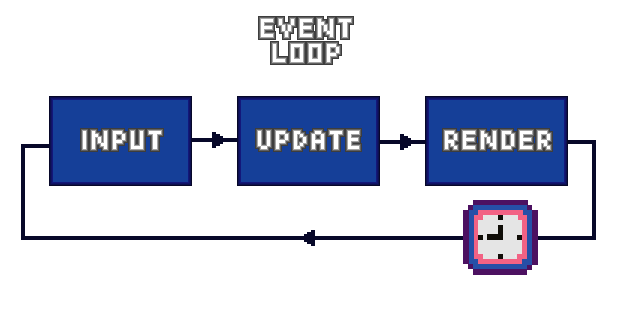
\includegraphics[width=1\linewidth]{figuras/event-loop.png}
    \caption{Event Loop}
    \label{fig:event-loopl}
\end{figure}

% Delta time
\subsection{Delta Time}
\label{sec:delta-time}
 \textit{Delta time} ou diferença de tempo é uma variável de controle que tem um valor numérico armazenado nela, esse valor corresponde a diferença de valores do ultimo \textit{clock} e o clock atual.
 \begin{equation}
    \Delta t = t' - t
    \label{eq:dt_equation}
\end{equation}

 Quando dizemos que um jogo roda a 30 quadros por segundo, temos o valor do delta é \(\frac{1}{30}\) isso significa também dizer que o game loop do jogo leva \(\frac{1}{30}\) segundos para ser executado, isso é utilizado para resolver o problema a evolução dos computadores criou, onde se tinha jogos feitos para máquinas quem tinham recursos escassos, e se um computador atual executasse um jogo dos anos 80 hoje sem nenhum mecanismo de controle, o jogo rodaria a alguns milhares de quadros e a experiência não seria boa se não fosse utilizado desse \textit{pattern} de jogos, não existiria uma normalidade entre dispositivos.


% coisas para explicar?
% colocar um codigo com \href{https://pyga.me/docs/ref/music.html}{pygame.mixer.música} \href{https://pyga.me/docs/ref/draw.html}{pygame.draw} 
% \href{https://pyga.me/docs/ref/event.html}{pygame.event} 
% \href{https://pyga.me/docs/ref/font.html}{pygame.font} 
% \href{https://pyga.me/docs/ref/image.html}{pygame.image} 
% \href{https://pyga.me/docs/ref/key.html}{pygame.key} 
% \href{https://pyga.me/docs/ref/rect.html}{pygame.Rect} 
% \href{https://pyga.me/docs/ref/sprite.html}{pygame.sprite} 
% \href{https://pyga.me/docs/ref/surface.html}{pygame.Surface} 
% \href{https://pyga.me/docs/ref/transform.html}{pygame.transform} 
% \href{https://pyga.me/docs/ref/window.html}{pygame.Window} 
% completar aqui

%  ======================================= 2.3 Mapas =================================
\section{Mapas}
\label{sec-mapas}
% explicar oq e um editor de mapas

A maioria dos jogos tem seus cenários, esses ambientes são de suma importância pois são neles onde os jogadores passam a maior parte do tempo como falado na seção \ref{sec:rpg} os cenário é um artefato imprescindível na ambientação do jogo, eles não são desenhados de forma totalmente manual, existem ferramentas que auxiliam na sua criação, são nomeados os softwares editores de mapas.

Um Editor de mapas é uma ferramenta que ajuda os designers e desenvolvedores do jogos a criarem de forma visual e intuitiva os mapas dos seus jogos, praticamente todos os jogos usam uma ferramenta para esse propósito e existem editores 2D quanto 3D para essa finalidade, em 2D existe uma técnica denominada \textit{Tile-Based} essa técnica de desenvolvimento de jogos eletrônico onde o cenário é feito por pequenas imagens quadradas, retangulares ou hexagonais chamados \textit{tiles} (ladrilhos).
% citar jogos populares que utilizam essa técnica (dofus)

\subsection{Tiles e Tilesets}
\label{sec:tiles-e-tilesets}
Tilesets são coleções de pequenas imagens reutilizáveis chamados “tiles” organizadas em uma grade. Cada tile representa uma pequena parte do mundo do jogo. Um tile pode representar um pedaço de chão, um segmento de uma parede ou uma decoração. Ao combinar diferentes tiles em diferentes posições temos um cenário que pode ser utilizado como fase de um jogo é um recurso gráfico para desenhar níveis e outros componentes estáticos do seu jogo de forma rápida e eficiente, já que não é necessário desenhar toda a área jogável.
Na figura \ref{fig:tileset-orthogonal} temos um exemplo de tileset ortogonal para um jogo a câmera vista de cima, e \ref{fig:tileset-platform-orthghonal} ilustra um tileset ortogonal para jogos plataforma.
\begin{figure}[h!]
    \centering
    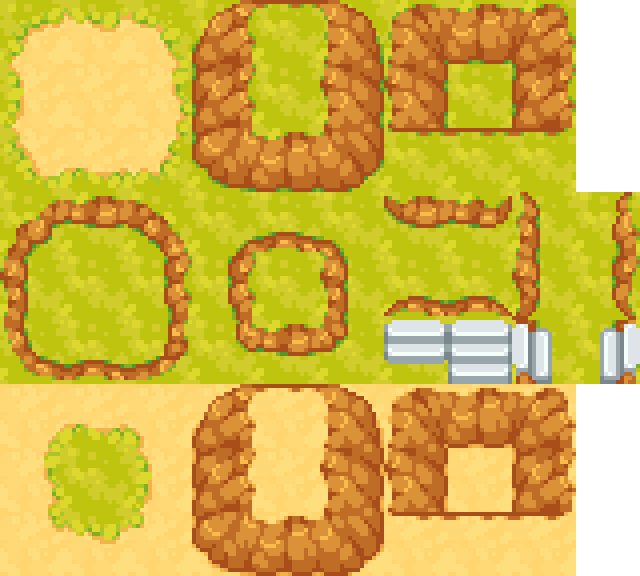
\includegraphics[width=0.5\linewidth]{figuras/tileset.png}
    \caption{Exemplo de Tileset Ortogonal}
    \label{fig:tileset-orthogonal}
\end{figure}
\begin{figure}[h!]
    \centering
    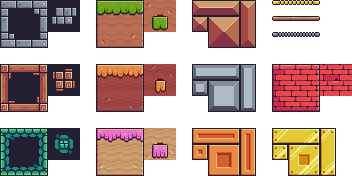
\includegraphics[width=0.5\linewidth]{figuras/tileset-orthogonal-platform.png}
    \caption{Exemplo de Tileset Ortogonal Para Jogos De Plataforma}
    \label{fig:tileset-platform-orthogonal}
\end{figure}

\subsection{Tiled}
\label{sec:tiled}
O Tiled \footnote{Tiled Map Editor \url{https://www.mapeditor.org}} é um editor de níveis 2D que ajuda game designers a desenvolverem o conteúdo de seus jogos. Seu recurso principal é editar mapas de tiles de várias formas, mas ele também suporta posicionamento de imagens livre, bem como maneiras eficientes de colocar metadados em seus sprites que futuramente poderão serem usados pela programação.
Camada de blocos

Ele suporta camadas de tiles retangulares retas e também camadas isométricas projetadas, isométricas escalonadas e hexagonais escalonadas. Um tileset pode ser uma única imagem contendo muitos tiles ou pode ser uma coleção de imagens individuais. Também é capaz de suportar algumas técnicas de simulação de profundidade através de deslocamento de camadas e alteração da ordem de renderização dos componentes.

O Tiled também suporta camadas de objetos, que podem ser usadas para colocar imagens, também é possível adicionar objetos como retângulos, pontos, elipses, polígonos, polilinhas e ladrilhos. O posicionamento de objetos não se limita à grade de ladrilhos e os objetos também podem ser dimensionados ou girados. As camadas de objetos oferecem muita flexibilidade para adicionar quase qualquer informação ao seu nível que seu jogo precise.
Na Figura \ref{fig:map-creation} temos a configuração inicial da criação de um mapa.
\begin{figure}[h!]
    \centering
    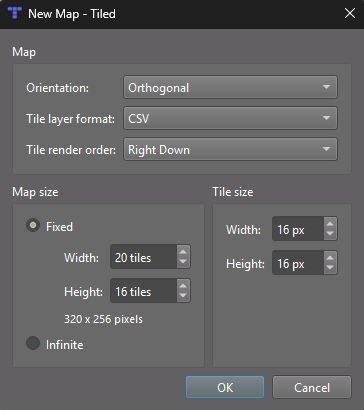
\includegraphics[width=0.5\linewidth]{figuras/new-map-tiled.png}
    \caption{Criação de mapa}
    \label{fig:map-creation}
\end{figure}

As características mais importantes a serem destacadas nessa tela são:
\begin{itemize}
    \item \textbf{Orientação (Orientation):} A orientação define como é o estilo de visualização do seu jogo, sendo possíveis 4 estilos “ortogonal”, “isométrico”, “escalonado” e “hexagonal”;
    \item \textbf{Tamanho do mapa \textit{(Map Size}):} nessa parte é definido o tamanho do mapa, é possível alterar os valores no decorrer da criação, o próprio software faz o calculo de quantos pixels o mapa ficará, na figura cada tile tem 32 píxels de tamanho, e o mapa é um quadrado 10 x 10 , sendo assim o tamanho final do mapa é 320 x 320
    \item \textbf{Tamanho do tile \textit{(Tile Size)}:}, essa é a informação mais importante dessa página, é nessa opção que se define o tamanho do tile que vai ser representado na tela, isso significa que cada azulejo do mapa terá exatamente esse tamanho, quando for a  hora de importar o tileset para o programa é importante garantir que o  tileset tem o mesmo tamanho do tile do mapa.
\end{itemize}
Com o mapa em branco criado agora é necessário importar um tileset para começar a desenhar o mapa a figura \ref{fig:new-tileset}  ilustra esse processo.
\begin{figure}[h!]
    \centering
    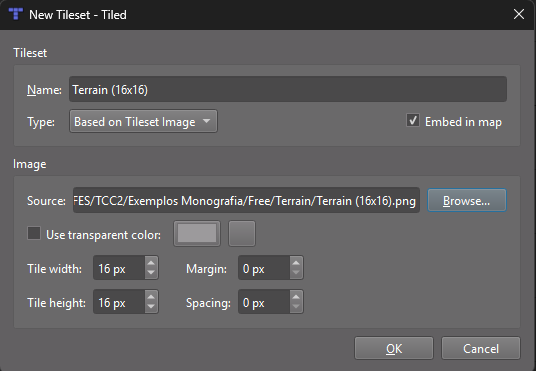
\includegraphics[width=0.5\linewidth]{figuras/new-tileset.png}
    \caption{Enter Caption}
    \label{fig:new-tileset}
\end{figure}
As Informações mais importantes aqui são:
\begin{itemize}
    \item \textbf{Procurar \textit{(Browse)}:} nessa opção você vai carregar o arquivo para o programa;
    \item \textbf{Tipo \textit{(Type)}:} aqui dizemos ao programa se é uma imagem única com múltiplos tilesets, ou uma imagem unica;
    \item \textbf{Largura do Tile e Altura do tile \textit{(Tile Width)} \textit{(Tile Height)}:} Nessa parte você está dizendo ao programa como "fatiar" a imagem que está recebendo, dividindo assim em vários azulejos únicos reutilizáveis, com essas configurações ficamos com um algo assim;
    \begin{figure}[h!]
        \centering
        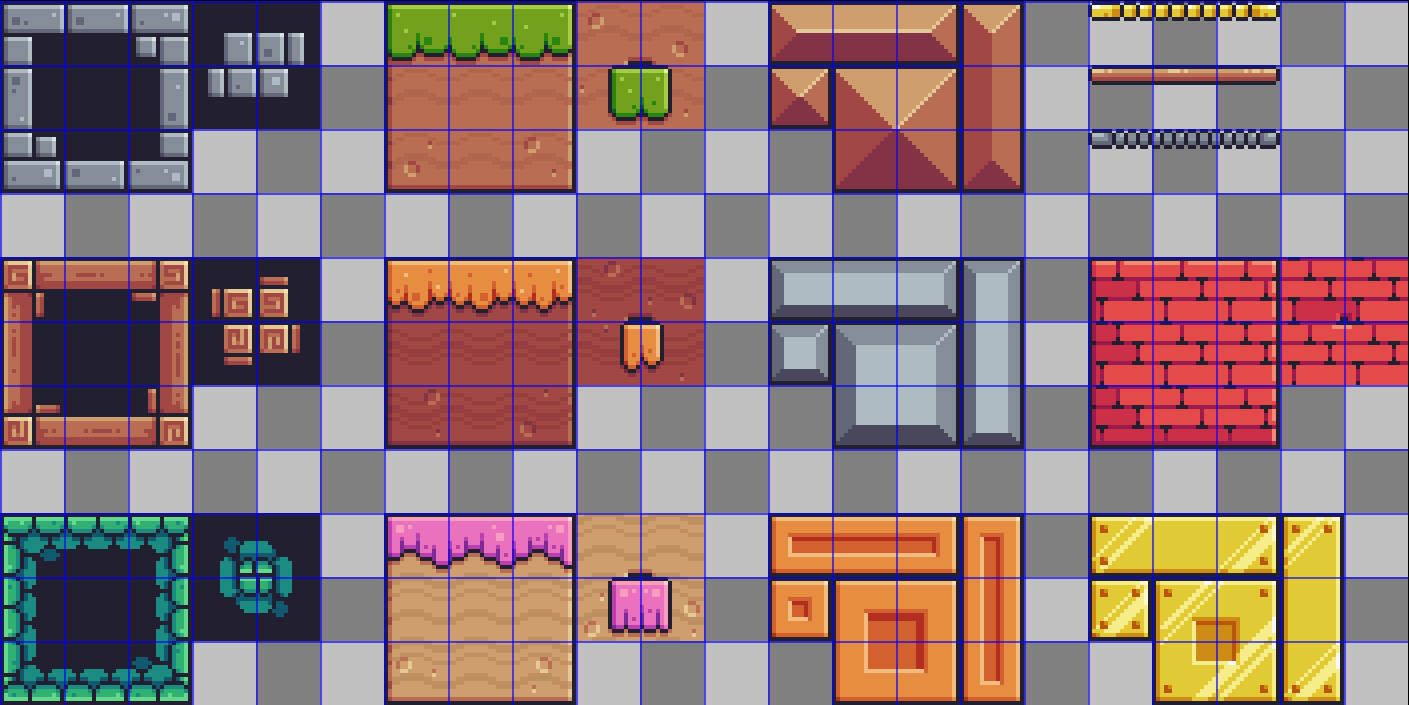
\includegraphics[width=0.8\linewidth]{figuras/tileset-dividido.png}
        \caption{Tileset dividido}
        \label{fig:tileset-dividido}
    \end{figure}
\end{itemize}

\subsection{Camadas}
\label{sec:camadas}
Antes de começar a desenhar nossos cenários é importante já ter definido de antemão quais serão as camadas utilizadas no projeto, para evitar o trabalho de ficar movendo objetos e tiles de uma camada a outra. Camadas ou \textit{layers} no tiled funcina definindo a ordem em que as coisas serão desenhadas na tela, de forma \textit{bottom-up} ou seja, os tiles serão renderizados de baixo para cima, onde, se tiver blocos sobrepostos, o que está mais acima tem prioridade. A figura \ref{fig:layers} mostra um mapa que tem quatro camadas, (i) terreno, (ii) topo do terreno (iii) objetos e (iv) entidades. 
\begin{figure}[h!]
    \centering
    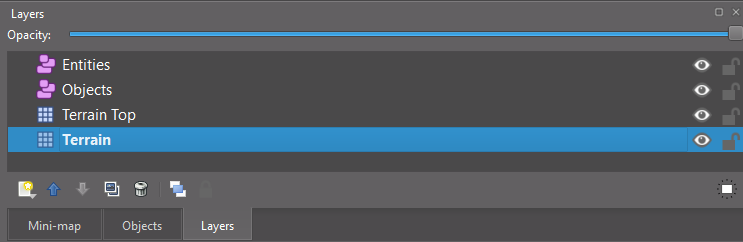
\includegraphics[width=1\linewidth]{figuras/layers.png}
    \caption{Camadas no Tiled}
    \label{fig:layers}
\end{figure}


Existem 4 tipos de camadas no Tiled sendo duas delas as utilizadas nesse trabalho  \textbf{(i) Camada de tiles}, é nela que é feita os terrenos do jogo bem como as coisas acima do terreno sem colisão (na figura \ref{fig:layers} as camadas "\textit{Terrain}" e "\textit{Terrain} Top", \textbf{(ii) camada de objetos} (Camadas "\textit{Entities}" e "\textit{Objects}" da figura
\ref{fig:layers} essa camada é muito útil pois o software permite adicionar metadados, dados com chave/valor aos dados presentes aqui, a figura \ref{fig:add-custom-property-object} exemplifica como adicionar uma propriedade "quebrável" a uma caixa.
\begin{figure}[h!]
    \caption{Adicionando uma propriedade personalizada a um objeto}
    \label{fig:add-custom-property-object}
    \subfloat{
        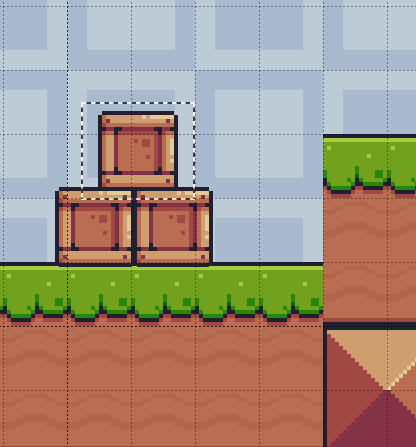
\includegraphics[width=0.35\linewidth]{figuras/example-map.png}
    }\hfill
    \subfloat{
        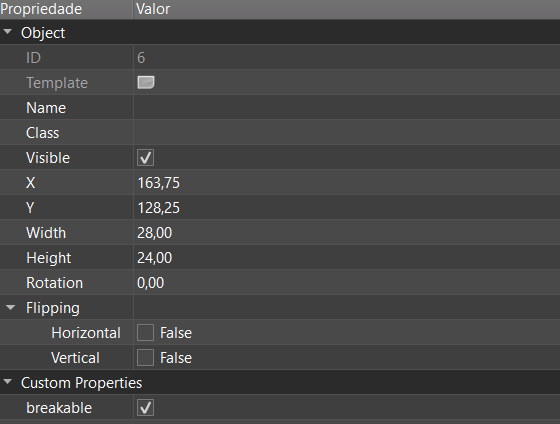
\includegraphics[width=0.5\linewidth]{figuras/custom-property.png}
    }
\end{figure}
Ao salvar essas configurações o programa gera um arquivo com a extensão '.tmx' que é o acrônimo de Translation Memory eXchange, é um formato baseado no 'xml' devido a isso faz o uso de tags e atributos de arquivo padrão usado na indústria de tradução para armazenar e trocar memórias de tradução, basicamente consiste em uma seção de cabeçalho, seguido por uma ou várias seções de corpo, cada uma contendo unidades de tradução. A listagem a seguir ilustra isso.

\newpage
\begin{lstlisting}[language=xml,breaklines, caption= example.tmx terrain layer]
<?xml version="1.0" encoding="UTF-8"?>
<map version="1.10" tiledversion="1.11.0" orientation="orthogonal" renderorder="right-down" width="20" height="16" 
tilewidth="16" tileheight="16" infinite="0" nextlayerid="5" nextobjectid="7">
 <tileset firstgid="1" name="Terrain (16x16)" tilewidth="16" tileheight="16" tilecount="242" columns="22">
  <image source="Free/Terrain/Terrain (16x16).png" width="352" height="176"/>
 </tileset>
 <tileset firstgid="243" name="images" tilewidth="28" tileheight="24" tilecount="1" columns="0">
  <grid orientation="orthogonal" width="1" height="1"/>
  <tile id="0">
   <image source="Free/Items/Boxes/Box1/Idle.png" width="28" height="24"/>
  </tile>
 </tileset>
 <tileset firstgid="244" name="Blue" tilewidth="16" tileheight="16" tilecount="16" columns="4">
  <image source="Free/Background/Blue.png" width="64" height="64"/>
 </tileset>
 <layer id="1" name="Terrain" width="20" height="16">
\end{lstlisting}

\begin{lstlisting}[language=xml,breaklines, caption= example.tmx object layer]
 <objectgroup id="3" name="Objects">
  <object id="4" gid="243" x="153" y="147.25" width="28" height="24"/>
  <object id="5" gid="243" x="172.5" y="147.25" width="28" height="24"/>
  <object id="6" gid="243" x="163.75" y="128.25" width="28" height="24">
   <properties>
    <property name="breakable" type="bool" value="true"/>
   </properties>
  </object>
 </objectgroup>
\end{lstlisting}


%  ======================================= PyTMX =======================================
\subsection{PyTMX}
\label{sec:pytmx}
% completar aqui
PyTMX\footnote{PyTMX \url{https://pytmx.readthedocs.io/en/latest/}} é um carregador de mapas para python/pygame projetado para jogos. Ele fornece carregamento inteligente de tiles com uma base de armazenamento rápida e eficiente. Ele manipula corretamente a maioria dos tipos de objetos Tiled, e também carrega metadados para eles, para que você possa modificar seus mapas e objetos no Tiled, em vez de modificar seu código-fonte ele inclui suporte completo para leitura desses dados para que possa definir parâmetros para coisas no Tiled, em vez de manter arquivos de dados externos, ou mesmo valores na fonte. Pytmx também é uma biblioteca e pode ser instalada por linha de comando com o pip, como exemplificado a seguir.
\begin{lstlisting}[language=bash,breaklines, caption= Instalação Pytmx]
pip install pytmx
\end{lstlisting}

\begin{lstlisting}[language=python,breaklines, caption= Uso Básico Pytmx]
import pytmx

tmxdata = pytmx.TiledMap("example.tmx")

print(tmxdata.width)
print(tmxdata.height)
print(tmxdata.tilewidth)
print(tmxdata.orientation)
print(tmxdata.layernames)
\end{lstlisting}

\begin{lstlisting}[language=bash,breaklines, caption= Saída]
>>> 20
>>> 16
>>> 16
>>> orthogonal
>>> {'Terrain': <TiledTileLayer[1]: "Terrain">, 'Terrain Top': <TiledTileLayer[2]: "Terrain Top">, 'Objects': <TiledObjectGroup[3]: "Objects">, 'Entities': <TiledObjectGroup[4]: "Entities">}
\end{lstlisting}

Para podermos usar esse mapa é necessário anteriormente importarmos ele para dentro do código isso é feito na linha 1, na linha 3 criamos uma variável para armazenar o mapa, e com isso temos acesso as informações presentes naquele mapa.

Agora para termos acesso aos metadados presentes na camada de objetos, por exemplo, podemos fazer uma iteração e verificação do nome do \textit{layer} com isso temos acesso aos objetos quebráveis.
\begin{lstlisting}[language=python,breaklines, caption= Verificação de Objetos Quebráveis]
for layer in tmxdata.visible_layers:
    if layer.name == 'Objects':
        for obj in layer:
            print(obj.properties['breakable'], obj.x, obj.y)
\end{lstlisting}

\begin{lstlisting}[language=bash,breaklines, caption= Saída]
>>> True 163.75 104.25
>>> True 152.25 123.0
>>> True 172.5 123.25
\end{lstlisting}










%  ======================================= Pixel Art ===================================
\section{Pixel Art}
\label{sec:pixel-art}
Pixel originada de (picture e element), ou seja, elemento de imagem sendo pix a abreviatura em inglês para pictures, é a menor unidade de uma imagem que e possível ser expressa digitalmente, se você fizer uma aproximação de uma foto digital ou de uma tela de celular, verá uma série de quadradinhos. Cada um deles é um pixel. A Pixel Art é um tipo de arte que usa pixels visíveis para compor uma imagem ou um vídeo, a junção de diversos pontos digitais de somado a criatividade e horas de dedicação proporciona obras de arte e animações que a ente humana não consegue acompanhar.

Em um monitor que permite imagens coloridas, cada pixel é composto por um conjunto de 3 pontos: vermelho, verde e azul. Nos melhores monitores, cada um desses pontos é capaz de exibir 256 tonalidades diferentes (o equivalente a 8 bits) com  a combinação dessas tonalidades dos três pontos é então possível exibir pouco mais de 16.7 milhões de cores diferentes (exatamente 16.777.216)  256 x 256 x 256, A quantidade de pixels a serem mostradas na tela depende do tamanho do display, por exemplo, em uma resolução HD (1280 x 720) temos 921.600 pixels, numa resolução 8K (7680 x 4320) temos 33.177.600 a serem preenchidos.

A pixel art surgiu nos anos 70 mas foi formalizada nos anos 80 nessa época era o início dessas tecnologia, os monitores ainda não possuíam a quantidade de pixels que temos atualmente. desenhar objetos na tela com "quadradinhos" era a única forma uma vez que era o único recurso que tinha na época mas que até nos dias atuais de forma despretensiosa é um estilo de arte que milhares de pessoas adoram 
nas figuras \ref{fig:mario} e \ref{fig:mega_man} vemos alguns exemplos de Pixel arts.
\begin{figure}[ht!]
    \caption{Exemplos de diferentes pixel arts em suas gerações esquerda Super Mario 8-bits (NES) /  Mega Man x4 32-bits (Playstation 1)}
    \label{fig:comparative-8bit-32-bit-pixel-art}
    \subfloat\label{fig:mario}1985.{
        
\includegraphics[width=0.35\linewidth]{figuras/mario-sprite-nes.png}
    }\hfill
    \subfloat\label{fig:mega_man}1998{
        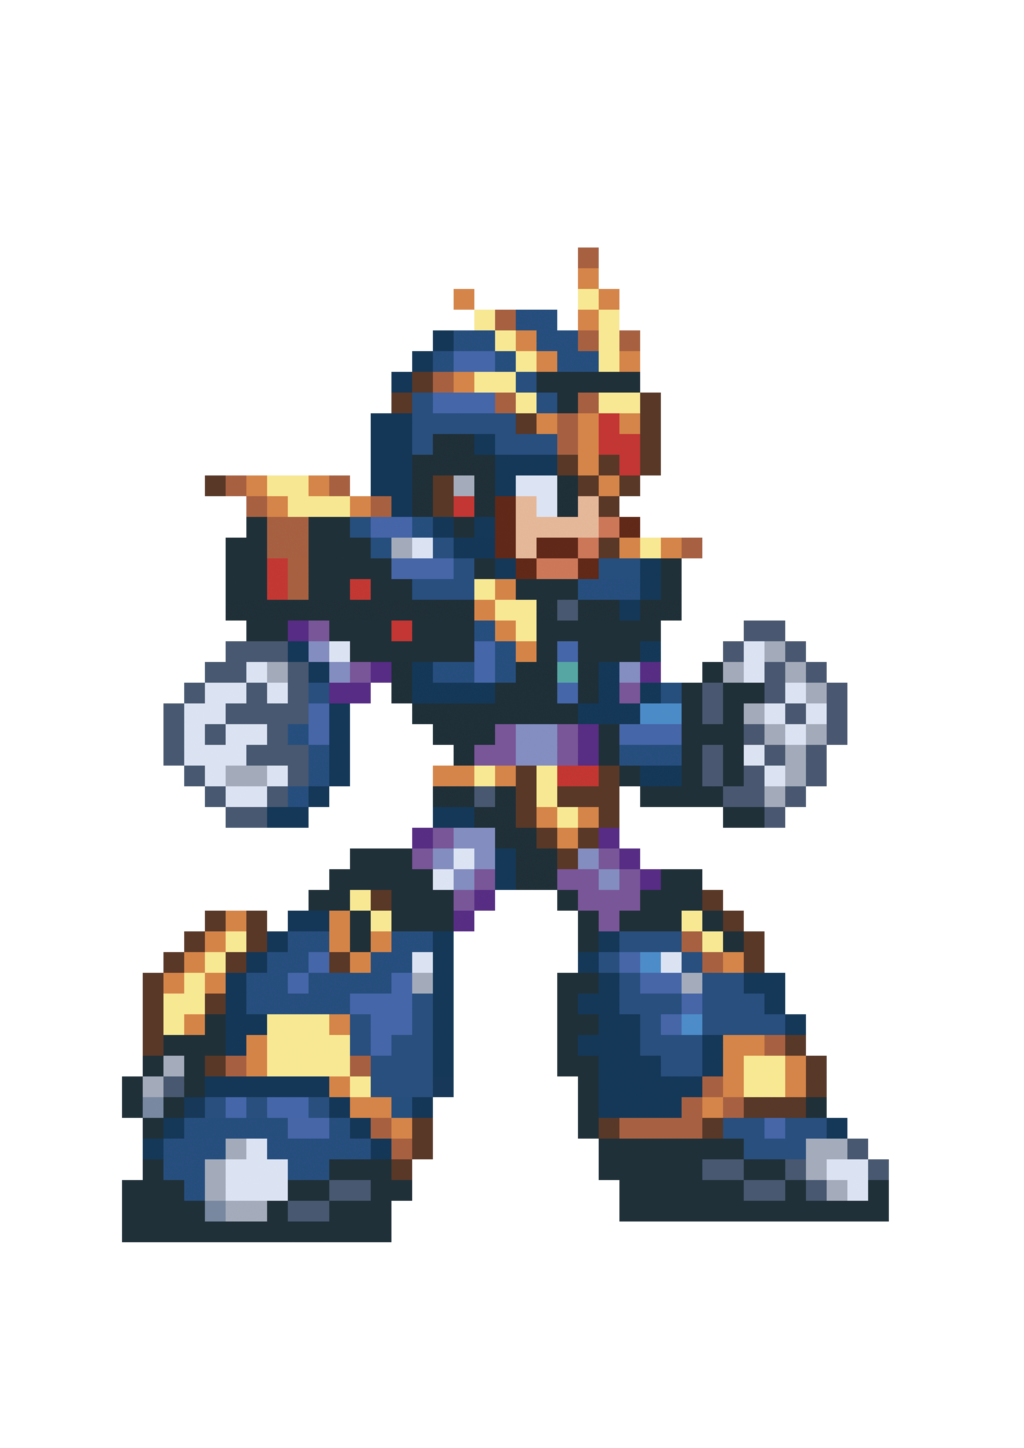
\includegraphics[width=0.3\linewidth]{figuras/mega-man-ps1.png}
    }
\end{figure}

\newpage
\subsection{Aseprite}  
\label{sec:aseprite}
% Para fazer um jogo é necessário ter sprites 
O Aseprite\footnote{Aseprite \url{https://www.aseprite.org}} é um software comercial especializado em pixel art, ele possui recursos e ferramentas específicas para essa finalidade permitindo assim a criação de animações 2D para videogames. De sprites a pixel-art, gráficos estilo retrô a figura \ref{fig:aseprite}. O software possui ferramentas para controlar
a animação quadro-a-quadro, rotações de pixel art pré-desenvolvidas, ferramentas que auxiliam na criação de tiles e tilesets
ilustra a tela básica do programa, a primeira vista ele é similar a outros programas de criação de imagens com exceção da grade quadriculada.  
\begin{figure}[ht!]
    \centering
    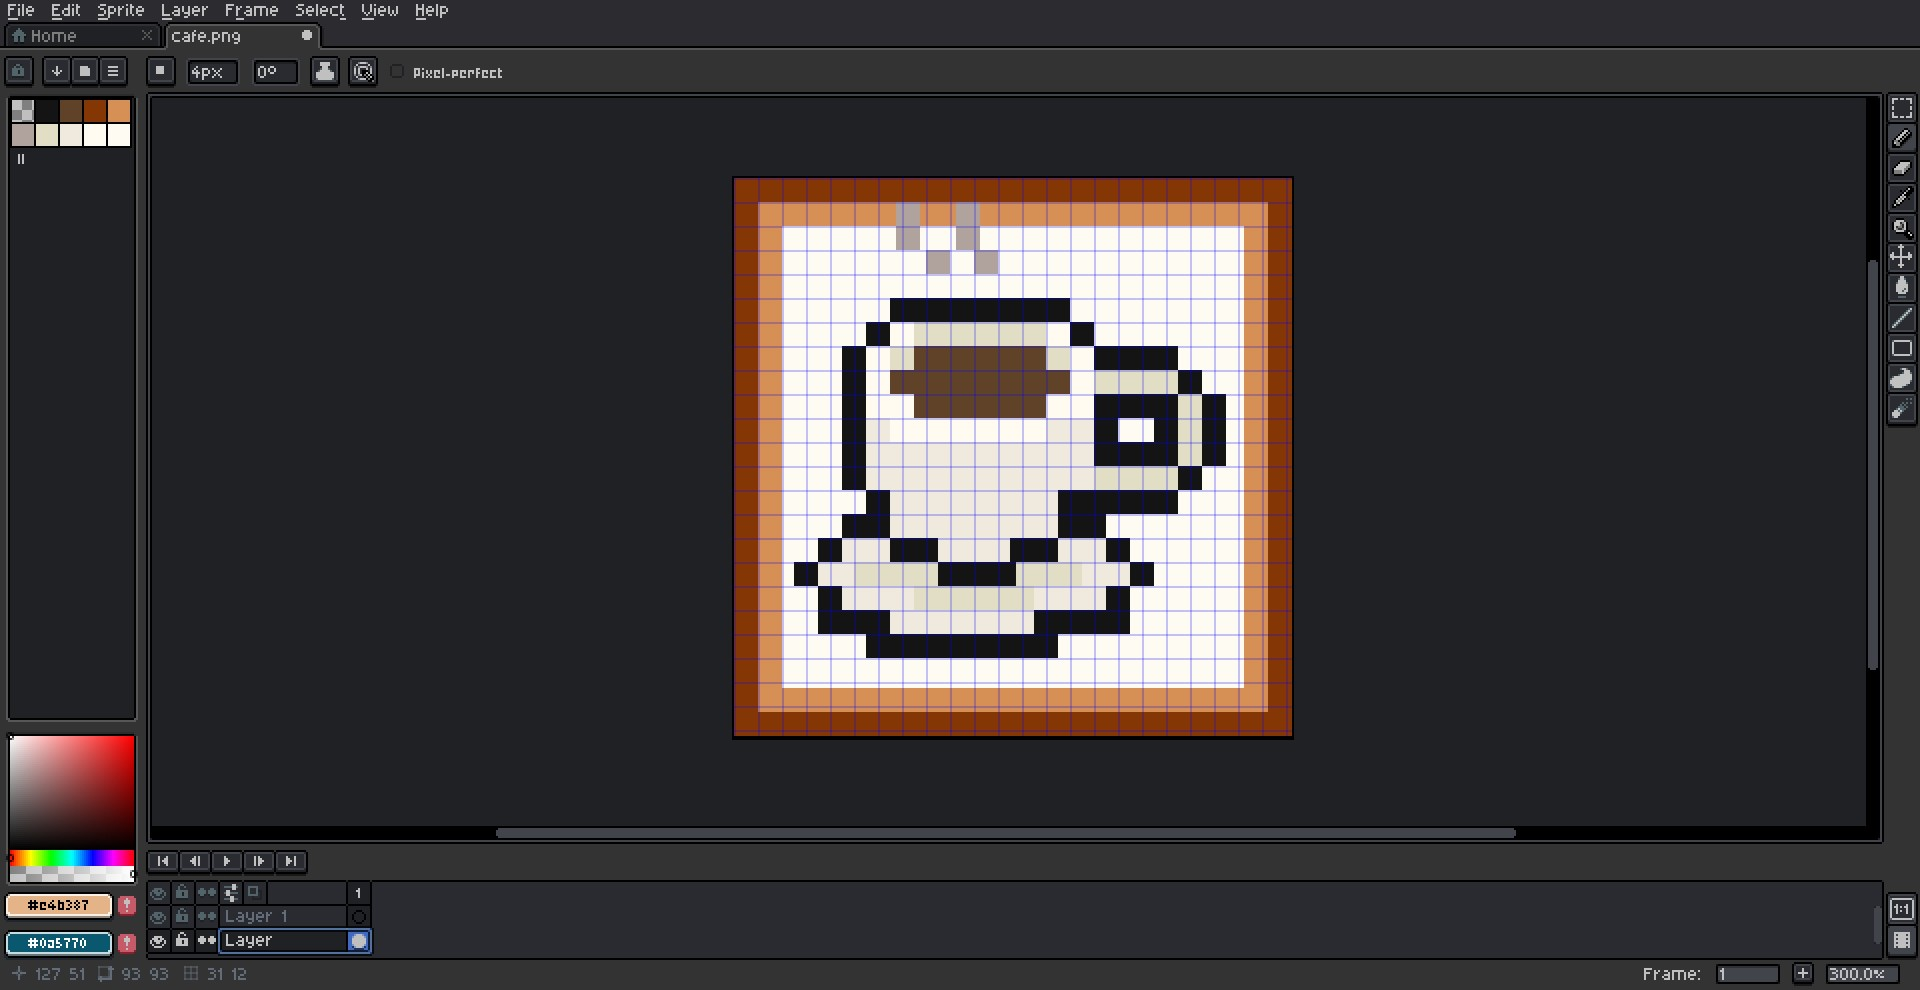
\includegraphics[width=1\linewidth]{figuras/aseprite.jpg}
    \caption{Visão Básica Aseprite}
    \label{fig:aseprite}
\end{figure}

Um Sprite é um objeto gráfico bidimensional (2D) usado em computação gráfica e particularmente em videogames. Ele normalmente consiste em uma imagem de bitmap ou uma série de imagens que são combinadas para criar uma animação. Um sprite pode ser pensado como uma entidade separada que existe dentro de uma cena maior, como um mundo de videogame. No Aseprite, um sprite consiste de uma sequência de quadros somados uma pilha de camadas. A intersecção de quadros e camadas cria uma matriz de células gráficas editáveis com imagens/pixels que podem ser editados com o editor de sprites . Camadas, quadros e células são visíveis na linha do tempo
\begin{figure}[h!]
    \centering
    
\includegraphics[width=1\linewidth]{figuras/sprite-frog.png}
    \caption{Ninja Frog Sprite de Pulo}
    \label{fig:enter-label}
\end{figure}
\subsection{Animação}
\label{sec:animacao}
 A animação é a ilusão de movimento que nossos cérebros nos enganam para perceber quando vemos vários quadros estáticos de obras de arte reproduzidos em rápida sucessão.
Um quadro é uma única imagem estática em um sprite, se adicionarmos e alterarmos os quadros a uma certa velocidade, cria-se a a impressão de movimento, essa impressão é chamada animação. 
Em programação existem varias formas de fazer a animação uma delas é através de vetores, a técnica consiste em carregar uma imagem e dizemos ao computador que queremos dividir essa imagem e armazena-lo num vetor, a figura \ref{fig:sprite-animation} exemplifica isso, nesse caso um vetor de duas linhas e cinco colunas, assim para fazer a animação desse personagem, basta percorrer as imagens alternadamente enquanto capturamos a entrada do jogador e vemos se é movimento

\begin{figure}[h!]
    \centering
    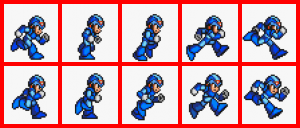
\includegraphics[width=0.8\linewidth]{figuras/megaman-sprite-animation-export.png}
    \caption{Sprite Animation}
    \label{fig:sprite-animation}
\end{figure}







% ==============================================================================
% PG - Nome do Aluno
% Capítulo 3 - Contribuição
% ==============================================================================
\chapter{Análise e Projeto}
\label{sec-contribuicao}

% Este capítulo deve apresentar a principal contribuição do trabalho. Caso o aluno e orientador desejem, o título do capítulo pode ser alterado para referenciar diretamente a contribuição (por exemplo, PIS: Plataforma para Integração de Serviços; Um Sistema para Controle de Processos da UFES, Solução de Otimização para Carregamento de Contêineres; etc.)

% O capítulo deve ser estruturado em seções de forma a apresentar de forma clara e com todas as informações necessárias, a contribuição do trabalho. Por exemplo, caso a contribuição produzida seja um sistema de informação, espera-se que sejam apresentados seus requisitos, funcionalidades, modelos (p.ex., modelo estrutural, modelo da arquitetura, etc.) e telas do sistema. Caso seja uma plataforma, espera-se que a plataforma como um todo seja apresentada e que seus componentes sejam descritos sejam apropriadamente.

Este capítulo tem o propósito de detalhar o escopo do jogo Super Labes World, aplicando os conceitos de engenharia de software para então identificar seus requisitos e finalmente criar o diagramas de classe. Na seção \ref{sec:descricao-do-cenario} fazemos uma breve explicação do cenário que foi incentivo para a criação desse trabalho, a seção \ref{sec:escopo} descreve o intuito desse trabalho, na seção \ref{sec:jogo} é descrito o design do jogo e também os possíveis usuários desse software, na seção \ref{sec:requisitos-do-jogo} é feito o levantamento de requisitos do jogo e com tudo isso em mãos, foi possível criar o diagrama de classes seção \ref{sec:diagrama-de-classes}.


\section{Descrição do Cenário}
\label{sec:descricao-do-cenario}
Alice, uma estudante hipotética recém-chegada ao curso de ciência da computação na UFES, sonhava em participar de projetos práticos que envolvessem programação e inovação e que fizessem diferença na sociedade. Com isso em mente, ela decide se candidatar ao LabES, um laboratório de extensão da UFES. Pouco tempo após preencher o formulário no site ela é contactada pela equipe responsável pelo embarque e rapidamente entra em um dos projetos.

Ao começar no projeto ela percebe que é a mais nova dentre os membros e não entende alguns termos e ferramentas utilizados entre eles; ela também percebe que há um grande volume de informações iniciais sobre o laboratório e também sobre o projeto. Pat, a professora coordenadora, Bob, membro sênior, junto aos demais estudantes do projeto, estão repletos de atividades e não conseguem dar atenção inicial necessária para ajudar Alice. Contudo, Alice é uma estudante dedicada e persegue os seus objetivos; diante dos desafios, ela elaborou um plano de estudos e o aplicava durante as noites. Após semanas de estudos, Alice começou a dar bons resultados no projeto.

Situações similares a esta ocorrem diariamente em vários laboratórios da UFES. Alguns estudantes, como Alice, conseguem se organizar de forma autônoma e, depois de algum tempo, passam a produzir para o projeto. Outros estudantes não têm a mesma resiliência e persistência de Alice e acabam desistindo no meio do caminho; ou então levam um tempo demasiado para conseguirem produzir, o que pode gerar uma certa desmotivação. Trata-se de um problema complexo, no qual que não existe um único culpado e nem um único ponto a ser resolvido. 

\section{Escopo}
\label{sec:escopo}
Diante da situação descrita na seção \ref{sec:descricao-do-cenario}, surge a ideia de criar o \textit{Super Labes World}, um jogo RPG \textit{desktop} desenvolvido com o intuito de ser uma ferramenta lúdica e didática, que possa ser utilizada para apoiar os estudantes em processos de ``embarque'' em laboratórios. A ideia é que o jogo possa ser usado para testar, reforçar e adquirir novos conhecimentos. Em sua versão inicial, o jogo foca em estudantes do LabES e, portanto, considera questões inerentes ao laboratório; porém, futuramente, com as devidas alterações/extensões, o jogo pode ser considerado para outros laboratórios e áreas da UFES.

\section{O Jogo}
\label{sec:jogo}

O jogo começa com o personagem acordando em sua casa e lembrando que precisa realizar um teste para entrar no projeto SigAMAES do LabES. Após este primeiro momento, a ambientação do jogo se passa na UFES. Durante a exploração inicial e interação com personagens, o jogador é dirigido ao prédio CT7, onde estão localizados o laboratório e os professores e, assim, pode começar a ``batalhar'' com alguns dos professores, que são os chefes a serem vencidos. A batalha é no estilo perguntas e respostas sendo que o jogador tem quatro opções para escolher. O tema das questões depende de cada professor, que são mestres em disciplinas específicas. Alguns exemplos de conteúdo de batalhas:

\begin{itemize}
    \item \textbf{Professor Vitor: }contém perguntas relacionadas a área de programação em java e conceitos de \textit{docker};
    \item \textbf{Professora Monalessa: }contém questões relacionadas a git, gitlab e gitflow;
    \item \textbf{Professora Patrícia: } contém as questões sobre a metodologia do LabES.
\end{itemize}

Ao final da batalha, caso o jogador vença, o professor entrega sua chave, representando a sua aprovação nesta disciplina. Somando as três chaves, o jogador pode finalmente ter acesso ao LabES. Caso o jogador erre mais do que 30\% das perguntas, a batalha é finalizada e o professor o instrui a utilizar o \textit{computador}. O \textit{computador} é uma mecânica do jogo que pode ser acessada a partir dos mapas ``sala do professor'' e ``labgrad'' e contém os \textit{links} para materiais de estudos abordados nas questões que o jogador errou. Ao clicar nesse \textit{link}, o jogador será redirecionado a esse conteúdo para estudar, aprender e tentar passar de nível novamente.

\subsection{Usuários}
\label{sec:usuarios}
O Super Labes World é uma versão inicial de um jogo que tem potencial de ser extensível. Foram identificados três potenciais usuários deste trabalho:

\begin{enumerate}
    \item \textbf{Estudantes da UFES que desejam iniciar no LabES:} O principal usuário do Super Labes World são estudantes da UFES que desejam iniciar ou são iniciantes no LabES. Toda a história, músicas, efeitos sonoros, interface, itens, questões, diálogos de personagens e personagens foram criados com isso em mente, de forma que o jogador possa se identificar e manter-se engajado no \textit{game}. 
    \item \textbf{Professores:} Um outro possível usuário do jogo são professores que podem alterar as perguntas e recriar o jogo, para diferentes propósitos. 
    \item \textbf{Estudantes de computação:} O jogo pode ser interessante para qualquer estudante de computação, uma vez que trata de questões da área.
\end{enumerate}

\section{Requisitos do Jogo}
\label{sec:requisitos-do-jogo}
A partir do escopo do projeto apresentado na seção \ref{sec:escopo}, os requisitos identificados foram organizados em tabelas. A tabela \ref{tbl-requisitos-funcionais} apresentada os requisitos funcionais e, na tabela \ref{tbl-requisitos-de-dominio}, os requisitos de domínio.

Um dos principais indicadores de sucesso de um sistema de software é o nível de atendimento aos requisitos para os quais foi projetado. Os requisitos de um sistema de software abrangem as descrições das funcionalidades que o sistema deve prover, e das restrições que devem devem ser atendidas. Em essência, os requisitos definem o que o sistema deve fazer e as
circunstâncias sob as quais deve operar. \cite{sommervilleengenharia}

Requisitos funcionais definem os serviços e tarefas que o sistema deve prover. Eles descrevem as funcionalidades específicas do software. Requisitos de domínio (ou regras de negócio) são provenientes do domínio de aplicação do sistema e expressam características e restrições próprias desse contexto. Eles são baseados no negócio que o sistema visa atender, podendo limitar requisitos funcionais já definidos ou estabelecer como cálculos específicos devem ser realizados, refletindo fundamentos do domínio de aplicação. \cite{sommervilleengenharia}.

 
\begin{table}[h!]
	\caption{Tabela de requisitos funcionais do Super Labes World.}
	\label{tbl-requisitos-funcionais}
	\centering
	\renewcommand{\arraystretch}{2}
	\begin{small}
		\begin{tabular}{ | p{20mm} | p{102mm} | p{20mm} |}\hline \rowcolor{MidnightBlue}
			\centering{\textbf{Id}} & \textbf{Descrição} & \textbf{Relação} \\\hline		
                \centering{RF1} & O jogo deve ser controlado pelo teclado &  \\\hline
			\centering{RF2} & O jogo deve ter um menu inicial. &  \\\hline
                \centering{RF3} & O jogo deve ter uma interface que mostre os controles do jogo. & RF2 \\\hline
			\centering{RF4} & O jogo deve ter uma tela que mostre os créditos. & RF2 \\\hline
                \centering{RF5} & Os cenários do jogo devem ser similares a UFES. &  \\\hline
			\centering{RF6} & Os \textit{sprites} dos professores devem ser minimamente similares com os professores reais. &  \\\hline
			\centering{RF7} & O jogo deve permitir o usuário abrir uma tela de inventário. & RF1 \\\hline
			\centering{RF8} & No inventário deve ser possível visualizar o nome descrição dos itens. &  RF1, RF7\\\hline
			\centering{RF9} & No inventário deve ser possível utilizar alguns itens. & RF1, RF7  \\\hline
			\centering{RF10} & O jogo deve permitir o usuário dialogar com personagens. & RF1 \\\hline
			\centering{RF11} & O jogo deve permitir o usuário interagir com alguns \textit{sprites}. &  RF1\\\hline
			\centering{RF12} & O jogo deve ter uma tela na qual seja possível acessar links para materiais de estudo. &  RF1\\\hline
			\centering{RF13} & O jogo deve permitir a transição entre mapas & RF1 \\\hline
                \centering{RF14} & O jogo ter um sistema de batalha de perguntas de múltipla escolha &  RF1\\\hline
                \centering{RF15} & As perguntas da batalha devem abordar questões relevantes para membros do LabES &  RF15\\\hline

		\end{tabular}
	\end{small}
\end{table}

\begin{table}[h!]
	\caption{Tabela de requisitos de domínio do Super Labes World.}
	\label{tbl-requisitos-de-dominio}
	\centering
	\renewcommand{\arraystretch}{2}
	\begin{small}
		\begin{tabular}{ | p{20mm} | p{122mm} | }\hline \rowcolor{MidnightBlue}
			\centering{\textbf{Id}} & \textbf{Descrição} \\\hline
                \centering{RN1} & A movimentação deve ser a partir dos direcionais e 'WASD' do teclado.\\\hline
			\centering{RN2} & O personagem principal deve colidir com outros \textit{sprites}.  \\\hline
			\centering{RN3} & Para o jogador interagir com os \textit{sprites} ele deve estar próximo a eles \\\hline
                \centering{RN4} & Durante a batalha o usuário deve receber feedback de resposta.  \\\hline
			\centering{RN5} & A batalha deve ser encerrada ao jogador errar 30\% da quantia total de perguntas.  \\\hline
			\centering{RN6} & Ao final da batalha se o jogador teve uma pontuação superior a 70\% ele deve ganhar um item que represente a sua vitoria nesse desafio.  \\\hline
			\centering{RN7} & Só deve ser possível o jogador zerar o jogo quando o jogador tiver todos os items dos professores  \\\hline
			\centering{RN8} & Ao jogador entrar em quaisquer interfaces o personagem deve ficar bloqueado, desbloqueando somente ao sair.  \\\hline


		\end{tabular}
	\end{small}
\end{table}


\clearpage
\section{Diagrama de Classes}
\label{sec:diagrama-de-classes}
% tabela com as classes
Um Diagrama de classes UML (\textit{Unified Modeling Language}) Linguagem de Modelagem Unificada é uma notação gráfica para modelagem de software. Essa linguagem define um conjunto de diagramas para documentar e ajudar no design de sistemas de software, particularmente sistemas orientados a objetos \cite{engsoftmoderna}. Esse tipo de modelagem e muito útil durante todo o desenvolvimento do sistema, porque auxilia os desenvolvedores a estruturar o sistema, identificar requisitos e remover os que não forem realmente necessários e ajudando na comunicação entre a equipe.

A Figura \ref{fig:diagrama-de-classes-uml} apresenta o diagrama de classes UML elaborado para representar os elementos utilizados na implementação do jogo. 

% escreva aqui um texto inicial explicando o diagrama, para o leitor conseguir começar a "leitura" do seu diagrama pelo lugar certo. POr exemplo: as classes centrais do diagrama são Game e Battle, que representam isso e aquilo. Um Game pode conter 0 ou mais batalhas; já uma batalha sempre pertence a um determinado jogo. Já uma Entidade representa <alguma coisa>, que pode ser isso ou aquilo... 

A classe central do jogo é \textit{Game}, é nela que está presente o \textit{game loop} e a instanciação para todas as demais classes. \textit{Battle} é a classe inclui a principal mecânica do jogo, as batalhas, podendo um jogo conter 0 ou n batalhas, o mesmo vale para as classes \textit{Character}, \textit{Sprite}, \textit{ChooseDialog} e \textit{DialogSprite} que também são possíveis várias instancias no mesmo jogo. As classes \textit{Computer}, \textit{Inventory}, \textit{AllSprites}, \textit{Timer}, \textit{Dialog} e \textit{Player} são apenas permitidas existirem uma por jogo. As demais classes serão um pouco mais detalhadas a seguir.


\begin{landscape}
\begin{figure}[h!]
    \centering
    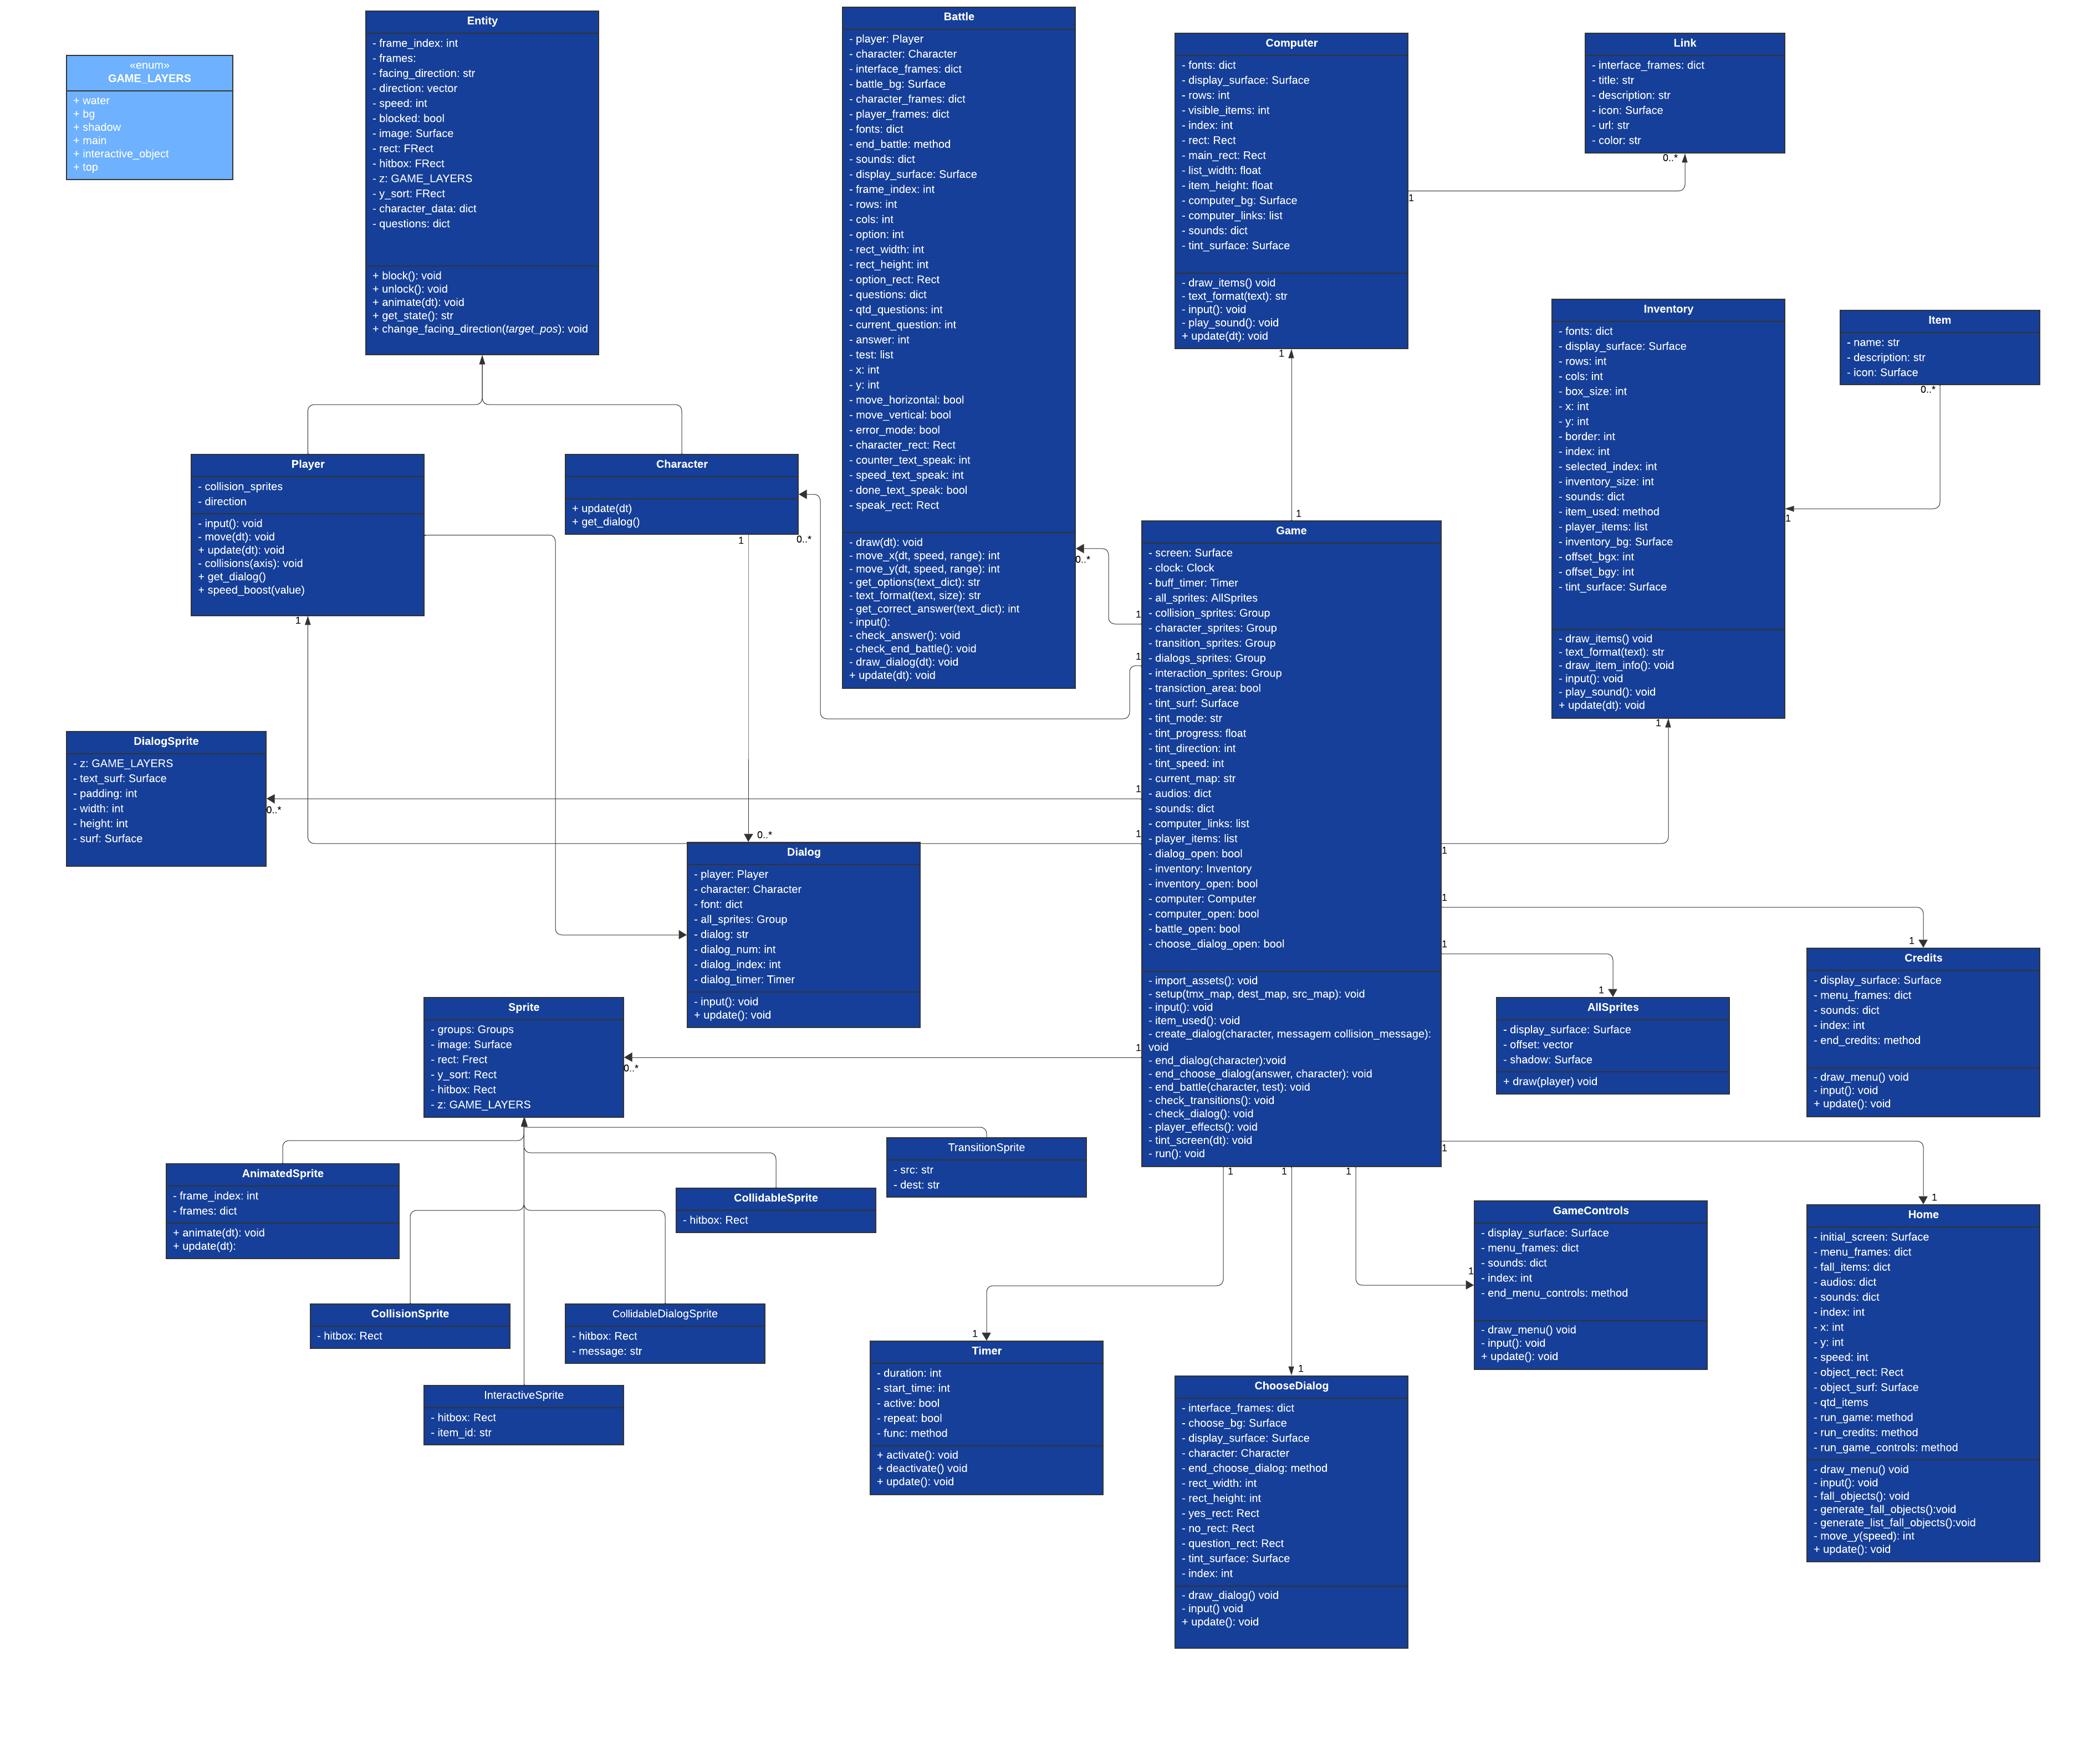
\includegraphics[width=0.8\linewidth]{figuras/diagrama-de-classes-uml.png}
    \caption{Diagrama de Classes do Super Labes World}
    \label{fig:diagrama-de-classes-uml}
\end{figure}
\end{landscape}

As tabelas \ref{tbl-especificacao-classes-1} e \ref{tbl-especificacao-classes-2}  apresentam mais informações sobre as classes propostas no diagrama.

\begin{table}[h!]
	\caption{Tabela especificando as classes do Super Labes World.}
	\label{tbl-especificacao-classes-1}
	\centering
	\renewcommand{\arraystretch}{2}
	\begin{small}
		\begin{tabular}{ | p{35mm} | p{100mm} |}\hline \rowcolor{MidnightBlue}
			\centering{\textbf{Classe}} & \textbf{Descrição}  \\\hline		
			\centering{\textit{AllSprites}} & Classe que representa a câmera do jogo. \\\hline
			\centering{\textit{Entity}} & Classe Pai usada para representar os personagens do jogo. Contém informações comuns a todas as entidades do jogo como frames, \textit{hitbox} e métodos relacionados a animação.   \\\hline
			\centering{\textit{Player}} & Classe filha de \textit{Entity}, representa o personagem que o jogador controla. Nele configuram-se atributos inerentes ao jogador, como a movimentação, colisão.  \\\hline
			\centering{\textit{Character}} & Classe filha de \textit{Entity} usada para representar os NPC's (Non Playable Character) ''personagens não jogáveis'' do jogo. Sua principal característica é o método para obtenção de diálogo relativo ao personagem.\\\hline
			\centering{\textit{Battle}} & Classe que representa a batalha do jogo. Contém todas as informações que fazem parte da batalha do jogo, destacando \textit{questions}, um dicionário com as questões relativas ao personagem e \textit{test}, uma lista que mantém um vetor de 0 para respostas erradas e 1 para respostas corretas.\\\hline
			\centering{\textit{Computer}} & Classe que representa a tela de visualização do computador do jogo. Contém o atributo \textit{computer\_links} que mantém um \textit{array} de \textit{Items} que serão mostrados ao entrar nessa tela. \\\hline
			\centering{\textit{Link}} & Representa um \textit{Link} do \textit{Computer}. Mantém informações que são utilizadas na interface \textit{Computer}. Sendo elas título, descrição, url, cor e icon que deve ser uma imagem 108 x 108 \\\hline
			\centering{\textit{Game}} & Classe que representa o jogo. Essa classe  mantém o \textit{main loop} e é responsável por carregar e armazenar todos os \textit{assets} e capturar o \textit{input} do jogador. \\\hline
			\centering{\textit{Inventory}} & Classe para representação da interface de inventário do jogador. \\\hline
			\centering{Item} & Classe que representa um Item do \textit{Inventory}. Mantém as informações dos items como nome, descrição e ícone, o tamanho ícone, que deve ser 93 x 93 \\\hline
		\end{tabular}
	\end{small}
\end{table}

\begin{table}[h!]
	\caption{Tabela com a continuação da especificação de classes do Super Labes World.}
	\label{tbl-especificacao-classes-2}
	\centering
	\renewcommand{\arraystretch}{2}
	\begin{small}
		\begin{tabular}{ | p{35mm} | p{100mm} |}\hline \rowcolor{MidnightBlue}
			  \centering{\textbf{Classe}} & \textbf{Descrição}  \\\hline
			\centering{\textit{DialogSprite}} & Classe que representa o dialogo do jogo. Ela realiza a renderização do diálogo na tela. \\\hline
			\centering{\textit{CollisionSprite}} & Classe filha de \textit{Sprite}, representa um sprite que pode ser colidido. Sua singularidade é ter uma \textit{hitbox}\\\hline
			\centering{\textit{CollidableSprite}} & Classe filha de \textit{Sprite}, representa um sprite que pode ser colidido, similarmente a \textit{CollisionSprite} porém a área de colisão dos \textit{sprites} nessa classe é menor.  \\\hline
			\centering{\textit{InteractiveSprite}} & Classe filha de \textit{Sprite}, representa um sprite interativo. Contém uma variável \textit{item\_id} que pode ser programada para diversos propósitos a partir de uma interação do jogador. \\\hline
			\centering{\textit{CollidableDialogSprite}} & Classe que herda \textit{Sprite}, usada para representar um diálogo caso jogador colide com determinadas posições do mapa. Essa classe não tem uma imagem associada e mantém uma mensagem que é disparada em colisões. \\\hline
			\centering{\textit{AnimatedSprite}} & Classe filha de \textit{Sprite}. Representa os \textit{Sprites} que animados do jogo. mantém um \textit{array} de \textit{frames} \\\hline
			\centering{\textit{TransitionSprite}} & Classe que herda \textit{Sprite}, representam os \textit{sprites} que levam para outros mapas. Guardam informações de origem e destino para poder realizar as transições entre mapas. \\\hline
			\centering{\textit{ChooseDialog}} & Classe que representa a interface de escolha do jogador antes de entrar em uma batalha. \\\hline
			\centering{\textit{Dialog}} & Classe pai que representa todos os diálogos do jogo. \\\hline
			\centering{\textit{Sprite}} & Classe Pai usada para representar todos os sprites do jogo. Suas informações são imagem, posição e camada. \\\hline
			\centering{\textit{Timer}} & Classe que representa o tempo no jogo. Responsável por realizar os controles de tempo do jogo. \\\hline
			  % \centering{\textbf{Classe}} & \textbf{Descrição}  \\\hline
			\centering{\textit{Home}} & Classe que representa a interface do menu inicial. \\\hline
			\centering{\textit{GameControls}} & Classe que representa a interface de controles do jogo, que pode ser acessada a partir da tela inicial. \\\hline
			\centering{\textit{Credits}} & Classe que representa a interface da tela de créditos que apenas pode ser acessada a partir da tela inicial.\\\hline
		\end{tabular}
	\end{small}
\end{table}

\clearpage
\section{Conclusões do Capítulo}
\label{sec:conclusoes-do-capitulo-3}
Este capítulo apresentou diversos aspectos essenciais para o desenvolvimento do jogo proposto. Inicialmente, foi estabelecido um cenário que foi o motivador para criação desse trabalho, nele é fornecido uma descrição objetiva do contexto em que o jogo está inserido. Essa definição facilita a compreensão dos desafios e metas a serem atingidos. Com isso foi possível definir o escopo que esse trabalho se propõe a atingir, bem como a história do jogo, e as suas principais mecânicas, e com isso foi feito o levantamento de requisitos.  

Por fim, foi apresentado o diagrama de classes, que desempenha um papel essencial na definição da estrutura do sistema. Com esse diagrama, foram identificadas as classes que representam os elementos do sistema e as relações entre elas. Esse diagrama junto a tabela de especificação de classes ajudaram na representação visual e facilitaram a compreensão das entidades do sistema e suas interações, auxiliando no planejamento para a implementação do sistema.


\chapter{Implementação}
\label{sec-implementacao}
Após a definição do escopo \ref{sec:escopo}, dos requisitos \ref{sec:requisitos-do-jogo}, do diagrama de classes \ref{sec:diagrama-de-classes}, da ideia do jogo \ref{sec:jogo}, do ferramental teórico e prático que será utilizado no desenvolvimento do trabalho \ref{sec-referencial} e uma motivação bem definida, temos uma base sólida para a implementação. Neste capítulo são apresentados os detalhes relacionados à implementação do software desenvolvido, bem como algumas das decisões de implementação tomadas com base na seção anterior. O objetivo deste capítulo é fornecer uma visão clara e detalhada de como o software foi estruturado e construído, demonstrando as escolhas técnicas realizadas para atender aos requisitos definidos previamente.

\section{Definições Iniciais}
Antes de começar um jogo \textit{pixel art} é importante definir qual vai ser o tamanho de cada \textit{tile}, os tamanhos mais comuns são 16 x 16, 32 x 32 e 64 x 64, para esse trabalho foi optado o tamanho 64 x 64. É importante que todos os tiles presentes no jogo respeitem o mesmo tamanho para uma melhor harmonia visual, e proporções de objetos compatíveis.

\section{Principais Funções}
Nessa seção serão detalhadas as principais funções que garantem o funcionamento adequado do software desenvolvido, a abordagem inclui uma explicação minuciosa sobre os módulos centrais abordando suas finalidades, interações e relevância para o cumprimento dos objetivos do sistema. Além disso, serão discutidas as escolhas realizadas durante o desenvolvimento, evidenciando como essas funções se complementam.

Antes de tudo, a primeira coisa a se fazer em um projeto Pygame é inicializa-lo \textit{pygame.init()} isso inicializará todos os módulos do Pygame e permitirá chamadas de funções do Pygame. Ao executar o programa a primeira tela que aparece ao jogador é a \textit{home}, essa tela pode levar a quatro outras possíveis transições sendo elas:
\begin{enumerate}
    \item \textbf{\textit{New: }} Começa um novo jogo;
    \item \textbf{\textit{Credits: }} Abre a tela de créditos;
    \item \textbf{\textit{Controls: }} Abre a tela de controles do jogo;
    \item \textbf{\textit{Exit: }} Sai do jogo;
\end{enumerate}

% Com isso feito é possível efetuar algumas configurações iniciais como por exemplo definir um título e redimensionar o tamanho da janela do jogo, esse passo é realizado somente em \textit{home} como mostra a listagem \ref{lst-home} a tela inicial do jogo, aqui na main \ref{lst-main} é apenas feita as chamadas para cada transição, sendo quatro possíveis i) iniciar um novo jogo; ii) abrir a tela de créditos; iii) abrir a tela de controles do jogo e iv) sair do jogo. 

Para gerenciar essas transições são criadas três variáveis de controle \textit{home\_open, credits\_open} e \textit{controls\_open} na main, todas do tipo \textit{bool}. Elas servem para definir qual aba estará sendo renderizada, não sendo possível mais de uma delas serem verdadeiras simultaneamente. Após isso são instanciados três objetos \textit{Home}, \textit{Credits} e \textit{Controls} que são as classes que contém as definições da respectiva tela, a variável de controle \textit{home\_open} é a única inicializada como verdadeiro pois é a tela que é mostrada inicialmente. Esse programa fica em um \textit{loop} enquanto captura os eventos e \textit{inputs} do jogador na tela inicial como mostra a listagem \ref{lst-main}.
\lstinputlisting[label=lst-main, caption=Main, language=Python, float=htpb]{codigos/main.py}

A troca de contexto é feito a partir das funções de \textit{callback} \textit{run\_game}, \textit{run\_credits}, \textit{run\_game\_controls} 
. Dependendo da valor de \textit{index} o programa redireciona para uma tela diferente. A listagem \ref{lst-callback} mostra a definição da função de \textit{callback}, e a listagem \ref{lst-home}  mostra a classe \textit{Home} onde é executado esse processo.
\begin{lstlisting}[label= lst-callback,language=Python,breaklines, caption= Função de \textit{callback} responsávél por alterar a variável de controle.]
    def run_credits():
        global credits_open; credits_open = True
        global home_open; home_open = False
\end{lstlisting}

\lstinputlisting[label={lst-home}, caption=Home, language=Python, float=htpb]{codigos/home.py}
\clearpage
Em \textit{Home} é definido o tamanho da tela (1280 x 720), também é feita a importação de imagens, áudios que são utilizados nela.
% e a reprodução da musica (linha 9). O parâmetro ''-1'' da função \textit{play} diz ao interpretador Python para a música ficar em \textit{loop}. S
No Super Labes World, todos os sprites utilizados são  baseados na classe \textit{Rect}. Essa classe pode ser utilizada para desenhar retângulos em determinados pontos da tela, essa também contem outras funções uteis para o programador, como detecção de colisões entre retângulos. Sua especificação é a seguinte:
% podem ser baseados em figuras geométricas. se queremos desenhar uma imagem em um ponto específico, ou queremos posicionar um \textit{sprite} em determinado local, é possível utilizar a  classe \textit{Rect} para isso
\begin{itemize}
    \item \textit{\textbf{x:}} posição em x em que sera desenhado;
    \item \textit{\textbf{y:}} posição em y em que sera desenhado;
    \item \textit{\textbf{width:}} largura do retângulo;
    \item \textit{\textbf{height:}} altura do retângulo;
\end{itemize}

% akiiiiiiiiiiiiiiiiiiiiiii
Normalmente não queremos jogar com personagens que sejam retângulos, ou mesmo interagir com NPC's (\textit{Non Playable Character}) personagem não jogável que sejam quadrados ou círculos, então associamos imagens a retângulos no Pygame. O método \textit{pygame.image.load} permite carregar uma imagem para o Pygame passando o caminho do arquivo como parâmetro, o retorno é um objeto do tipo \textit{Surface}. A classe Surface no Pygame é utilizada  para a representação das imagens. A figura \ref{fig:player} mostra o resultado da associação de uma imagem a um retângulo.
\begin{figure}[h!]
    \centering
    
\includegraphics[width=0.5\linewidth]{figuras/player.png}
    \caption{Exemplo de retângulo associado a imagem do personagem principal, toda a area vermelha representa o retângulo associado ao \textit{player}}
    \label{fig:player}
\end{figure}

O método \textit{blit} do Pygame, é utilizado para desenhar imagens \textit{Surfaces} na tela. Essa função tem a seguinte assinatura.
\begin{itemize}
    \item \textit{\textbf{source}:} A imagem \textit{Surface} a ser desenhada sobre o \textit{Surface} atual;
    \item \textit{\textbf{dest (opcional):}} Posição onde será desenhado a imagem, sendo o padrão o canto superior esquerdo (0, 0);
    \item \textit{\textbf{area (opcional):}} A delimitação da área retangular para desenhar;
    \item \textit{\textbf{special\_flags (opcional):}} Controla como as cores do da imagem serão combinadas com a Superfície;
\end{itemize}

Na função \textit{draw\_menu} essa que é responsável por desenhar as informações na tela \textit{home} faz uso desse método, a imagem de \textit{background} é desenhada ao passar como parâmetro a imagem \textit{Surface} dessa interface. Para causar o efeito de iluminação sobre o index selecionado são usados também os parâmetros \textit{dest} e \textit{special\_flag}. O primeiro parâmetro é o ícone da imagem com o fundo branco, o segundo parâmetro é o retângulo com as coordenadas de onde está a seleção, este varia conforme o index, e o terceiro parâmetro é a \textit{special\_flag} \textit{BLEND\_RGB\_ADD }, essa \textit{flag} mistura os canais de cores RGB da imagem de \textit{background} com o ícone da imagem de fundo branco. A figura \ref{fig:blit-example} ilustra esse processo.

% a imagem de \textit{background} e os retângulos de seleção. Para causar o efeito de iluminação sobre os retângulos ao selecionar cada index é feito o uso do método \textit{blit} do pygame, esse método desenha uma imagem sobre outra imagem, sendo a primeira imagem o icone de exit com o fundo branco, e o destino onde será desenhado o retângulo com às coordenadas de cada botão, essa coordenada varia de acordo com o index. A fun tem a seguinte assinatura.
% % \begin{itemize}
% %     \item \textit{\textbf{source}:} A imagem \textit{Surface} a ser desenhada sobre o \textit{Surface} atual;
% %     \item \textit{\textbf{dest (opcional):}} Posição onde será desenhado a imagem, sendo o padrão o canto superior esquerdo (0, 0);
% %     \item \textit{\textbf{area (opcional):}} A delimitação da área retangular para desenhar;
% %     \item \textit{\textbf{special\_flags (opcional):}} Controla como as cores do da imagem serão combinadas com a Superfície;
% % \end{itemize}
% É graças ao quarto parâmetro \textit{special\_flags} que é possível causar esse efeito, usando a \textit{flag} \textit{BLEND\_RGB\_ADD } misturamos as cores RGB da mesma imagem com o fundo branco e é adicionado os canais de cor de origem aos canais de cor de destino.

\begin{figure}[h!]
    \centering
    
\includegraphics[width=1\linewidth]{figuras/blit_example.png}
    \caption{Exemplo de sobreposição de imagens com o método \textit{blit}}
    \label{fig:blit-example}
\end{figure}

A operação de \% (resto da divisão) é feita sobre o index para garantir que a opção selecionada pelo jogador seja somente uma das opções definidas. A variável \textit{new\_rect} contém o retângulo de coordenadas que será desenhado na tela. Todos os retângulos de seleção da tela inicial tem o tamanho fixo 123 x 90, o que muda é a posição que ele sera desenhado.

No Pygame um \textit{sprite} pode ser representado com a classe nativa \textit{Sprite}, herdar essa classe base e adicionar os atributos e métodos que são do nosso interesse é muito útil. Além disso o Pygame conta também com a classe \textit{Group}, nessa classe container é possível adicionar objetos do tipo \textit{Sprite}. A classe \textit{Group} pode ser utilizada para criar grupos de \textit{sprites} que o programador deseja que tenham comportamentos específicos. A classe suporta os seguintes operações padrão do Pygame.
\begin{itemize}
    \item \textbf{\textit{in:}}  testa se um Sprite está contido no grupo;
    \item \textbf{\textit{len:}}  retorna o número de Sprites contidos no grupo;
    \item \textbf{\textit{bool:}}  verifica se algum Sprite está contido no grupo;
    \item \textbf{\textit{iter:}}  itera todos os Sprite no grupo;
\end{itemize}

% especialmente se usada em conjunto com a classe container \textit{Groups}. Nessa classe é possível adicionar Sprites que podem ser criados para comportamentos específicos, por exemplo, se queremos criar um grupo de sprites que tenham o comportamento de matar o jogador em caso de colisão, poderíamos criar um \textit{Group} chamado \textit{''hitkill\_sprites''} e nele adicionar todos os sprites que queremos que tenha esse comportamento. Para realizar a ação de matar o \textit{player} bastaria percorrer \textit{hitkill\_sprites} e verificar a colisão, 

% veja no exemplo da listagem \ref{lst:hitkill-sprite}
% \lstinputlisting[label=lst:hitkill-sprite, caption=\textit{Hitkill Sprites}, language=Python, float=htpb]{codigos/hitkill_sprites.py}
\lstinputlisting[label=lst:game, caption=Classe \textit{Game}, language=Python, float=htpb]{codigos/game.py}

No jogo existem cinco tipos de \textit{Groups} podendo um \textit{sprite} pertencer a mais de um grupo simultaneamente, a (listagem \ref{lst:game}) mostra a classe \textit{Game} onde é feito o uso recurso:
\begin{itemize}
    \item \textit{\textbf{collision\_sprites: }}Grupo que contém todos os \textit{sprites} colidíveis do jogo no mapa atual;
    \item \textit{\textbf{character\_sprites: }}Grupo que contém todos os \textit{sprites} de personagens do game no mapa atual;
    \item \textit{\textbf{transition\_sprites: }}Grupo que contém todos os \textit{sprites} de colisão no mapa atual;
    \item \textit{\textbf{dialogs\_sprites: }}Grupo que contém todos \textit{sprites} que geram uma caixa de diálogo no mapa atual;
    \item \textit{\textbf{interaction\_sprites: }}Grupo que contém todos os \textit{sprites} do jogo que são interativos;
\end{itemize}

A classe \textit{Game} também responsável por inicializar todas as variáveis, áudios, e \textit{assets} que são pertinentes ao jogo. É nessa classe que são chamadas as função \textit{import\_assets} e \textit{setup}, sendo a primeira para carregar todos os \textit{assets} do jogo para o programa, e a segunda para fazer a inicialização do mapa inicial. 

% inicial do jogador essa será explicada na listagem \ref{lst-import-assets} e chama também o método \textit{setup} listagem \ref{lst-setup} que que carrega e inicializa o mapa inicial.


\lstinputlisting[label=lst-import-assets, caption=Import Assets, language=Python, float=htpb]{codigos/import_assets.py}
\clearpage
O método \textit{import\_assets} (listagem \ref{lst-import-assets}) é responsável por fazer a importação e alocação de todos os mapas e assets do jogo. A atribuição desses \textit{assets} é feita através de um dicionário para melhor organização do código. Abaixo na tabela \ref{tbl-especificacao-dicionario} da especifica mais as possíveis chaves e valores.


\begin{table}[h!]
	\caption{Especificação dos dicionários de assets.}
	\label{tbl-especificacao-dicionario}
	\centering
	\renewcommand{\arraystretch}{2}
	\begin{small}
		\begin{tabular}{ | p{35mm} | p{35mm} | p{65mm} |}\hline \rowcolor{MidnightBlue}
                \hline
                Variável & Chave & Valor \\
                \hline
                \textit{tmx\_maps} & \textit{map\_name} & Arquivo TMX \\ 
                \hline
                \multirow{3}{4em}{overworld\_frames} 
                & \textit{characters} & \textit{Sprites} de personagems \\ 
                & \textit{water} & \textit{Sprites} de água \\ 
                & \textit{lake} & \textit{Sprites} das bordas do lago \\ 
                \hline
                \multirow{3}{4em}{fonts} 
                & \textit{dialog} & Fonte do diálogo \\ 
                & \textit{bold} & Fonte negrito \\ 
                & \textit{regular} & Fonte do inventário e computador \\ 
                & \textit{regular\_mid} & Fonte igual a anterior com tamanho 22 \\ 
                & \textit{regular\_big} & Fonte igual a anterior com tamanho 34 \\ 
                \hline
                \multirow{3}{4em}{interface\_frames} 
                & \textit{interface} & \textit{Sprites} com os \textit{layouts} da interface \\ 
                & \textit{items} & \textit{Sprites} com os items do inventario \\ 
                & \textit{interactive\_objects} & \textit{Sprites} que tem algum tipo de animação ao interagir \\ 
                \hline

                \end{tabular}
	\end{small}
\end{table}

\clearpage
\lstinputlisting[label=lst-setup, caption=Setup, language=Python, float=htpb]{codigos/setup.py}
\clearpage
O método a anterior \textit{setup} (listagem \ref{lst-setup}) tem a função de carregar o mapa passado como parâmetro e iniciar todos os \textit{sprites} presentes no mapa passado como argumento. Essa função é chamada ao iniciar um novo jogo, e também caso o jogador mude para outro mapa do \textit{game}. Como pode conter um mapa na memória quando essa função for chamada, o primeiro passo é limpar os \textit{sprites} do mapa anterior. Após isso é feito uma série de interações sobre todas as camadas presentes no mapa \textit{.tmx} que foram criadas no editor de mapas. É nessa etapa que é realizada a atribuição de cada \textit{sprite} com os seus respectivos grupos, sendo eles.
\begin{table}[h!]
	\caption{Tabela especificando os tipos de \textit{sprites} presentes em Super Labes World}
	\label{tbl-especificacao-sprites}
	\centering
	\renewcommand{\arraystretch}{3}
	\begin{small}
		\begin{tabular}{ | p{37mm} | p{23mm}  | p{52mm} | p{30mm} | }\hline \rowcolor{MidnightBlue}
			\centering{\textbf{Classe}} & \centering{\textbf{Camadas}} & \textbf{Descrição} & \textbf{Grupos} \\\hline		
                \centering{\textit{Sprite}} & \centering{\textit{Terrain, Terrain Top, Terrain Objects}} & {Classe com os tiles da camada mais baixa sem colisões} & {\textit{all\_sprites}} \\\hline
                \centering{\textit{AnimatedSprite}} & \centering{\textit{Lake, Lake Edges}} & {Classe com tiles animados do lago sem colisão} & {\textit{all\_sprites}} \\\hline			
                \centering{\textit{CollidableSprite}} & \centering{\textit{Objects}} & {Classe com os sprites de objetos do jogo com colisão} & {\textit{all\_sprites, collision\_sprites}} \\\hline		
                \centering{\textit{InteractiveSprite}} & \centering{\textit{Interactive Objects}} & {Classe com os sprites com interação com colisão} & {\textit{all\_sprites, collision\_sprites, interactive\_sprites}} \\\hline	
                \centering{\textit{CollisionSprite}} & \centering{\textit{Collisions}} & {Classe com as colisões sem uma imagem} & {\textit{collision\_sprites}} \\\hline		
                \centering{\textit{CollidableDialogSprite}} & \centering{\textit{Dialogs}} & {Classe com os sprites de diálogo} & {\textit{dialog\_sprites}} \\\hline		
                \centering{\textit{TransitionSprite}} & \centering{\textit{Transitions}} & {Classe que armazena os sprites de transição sem imagem} & {\textit{transition\_sprites}} \\\hline		
                \centering{\textit{Player}} & \centering{\textit{Entities}} & {Classe do jogador principal} & {\textit{all\_sprites}} \\\hline			
		\end{tabular}
	\end{small}
\end{table}
\begin{table}[h!]
	\caption{Tabela especificando os tipos de \textit{sprites} presentes em Super Labes World}
	\label{tbl-especificacao-sprites}
	\centering
	\renewcommand{\arraystretch}{3}
	\begin{small}
		\begin{tabular}{ | p{37mm} | p{23mm}  | p{52mm} | p{30mm} | }\hline \rowcolor{MidnightBlue}
			\centering{\textbf{Classe}} & \centering{\textbf{Camadas}} & \textbf{Descrição} & \textbf{Grupos} \\\hline	
                \centering{\textit{Character}} & \centering{\textit{Entities}} & {Classe para representar as entidades de personagens do jogo} & {\textit{all\_sprites, collision\_sprites, characters\_sprites}} \\\hline	
		\end{tabular}
	\end{small}
\end{table}

\section{Personagens}
Os personagens de um jogo são uma peça fundamental especialmente para um jogo do gênero RPG, eles desempenham um papel central na construção da experiência narrativa e interativa e enriquecem fortemente a ambientação do jogo, esse capítulo vai abordar em mais detalhes como foi feita a criação de personagens

Os \textit{sprites} dos personagens do jogo foram desenhados no software Aseprite discutido na seção \ref{sec:aseprite} e exportados para o formato PNG (Portable Network Graphics). Cada \textit{sprite} de personagem tem o tamanho (512 x 512), mas no programa essa imagem é subdividida em 16 quadrados de tamanhos iguais (128 x 128) como mostra a figura \ref{fig:player-animation}

A adição de personagens ao jogo é feita pela ferramenta Tiled citado na seção \ref{sec:tiled}. No software existe um recurso chamado \textit{Insert Point}, os pontos são os objetos mais simples possíveis de adicionar a um mapa, eles representam apenas uma localização e não podem ser redimensionados ou girados, mas é possível atribui-los com metadados. Esses metadados podem ser utilizados no Pygame para a identificação de cada personagem. Em nosso caso os metadados inseridos foram, e pode ser vista pelas figuras \ref{fig:tiled-house} e \ref{fig:tiled-player-properties}.
\begin{itemize}
    \item \textbf{\textit{character\_id: }} Identificador do personagem. Todas as características do personagem (diálogos, \textit{frames}, questões, etc) são dependentes desse \textit{id} ;
    \item \textbf{\textit{direction: }}Define qual é a direção inicial do jogador;
    \item \textbf{\textit{pos: }} Contém o mapa anterior que o \textit{player} estava antes da transição. Isso é necessário porque todo mapa contém pelo menos duas possíveis transições (ida e volta). Essa variável então é usada para diferenciar cada posição do jogador e o programa conseguir desenhar o jogador na posição correta. (Propriedade é relativa somente ao player);
\end{itemize}

\begin{figure}[h!]
    \centering
    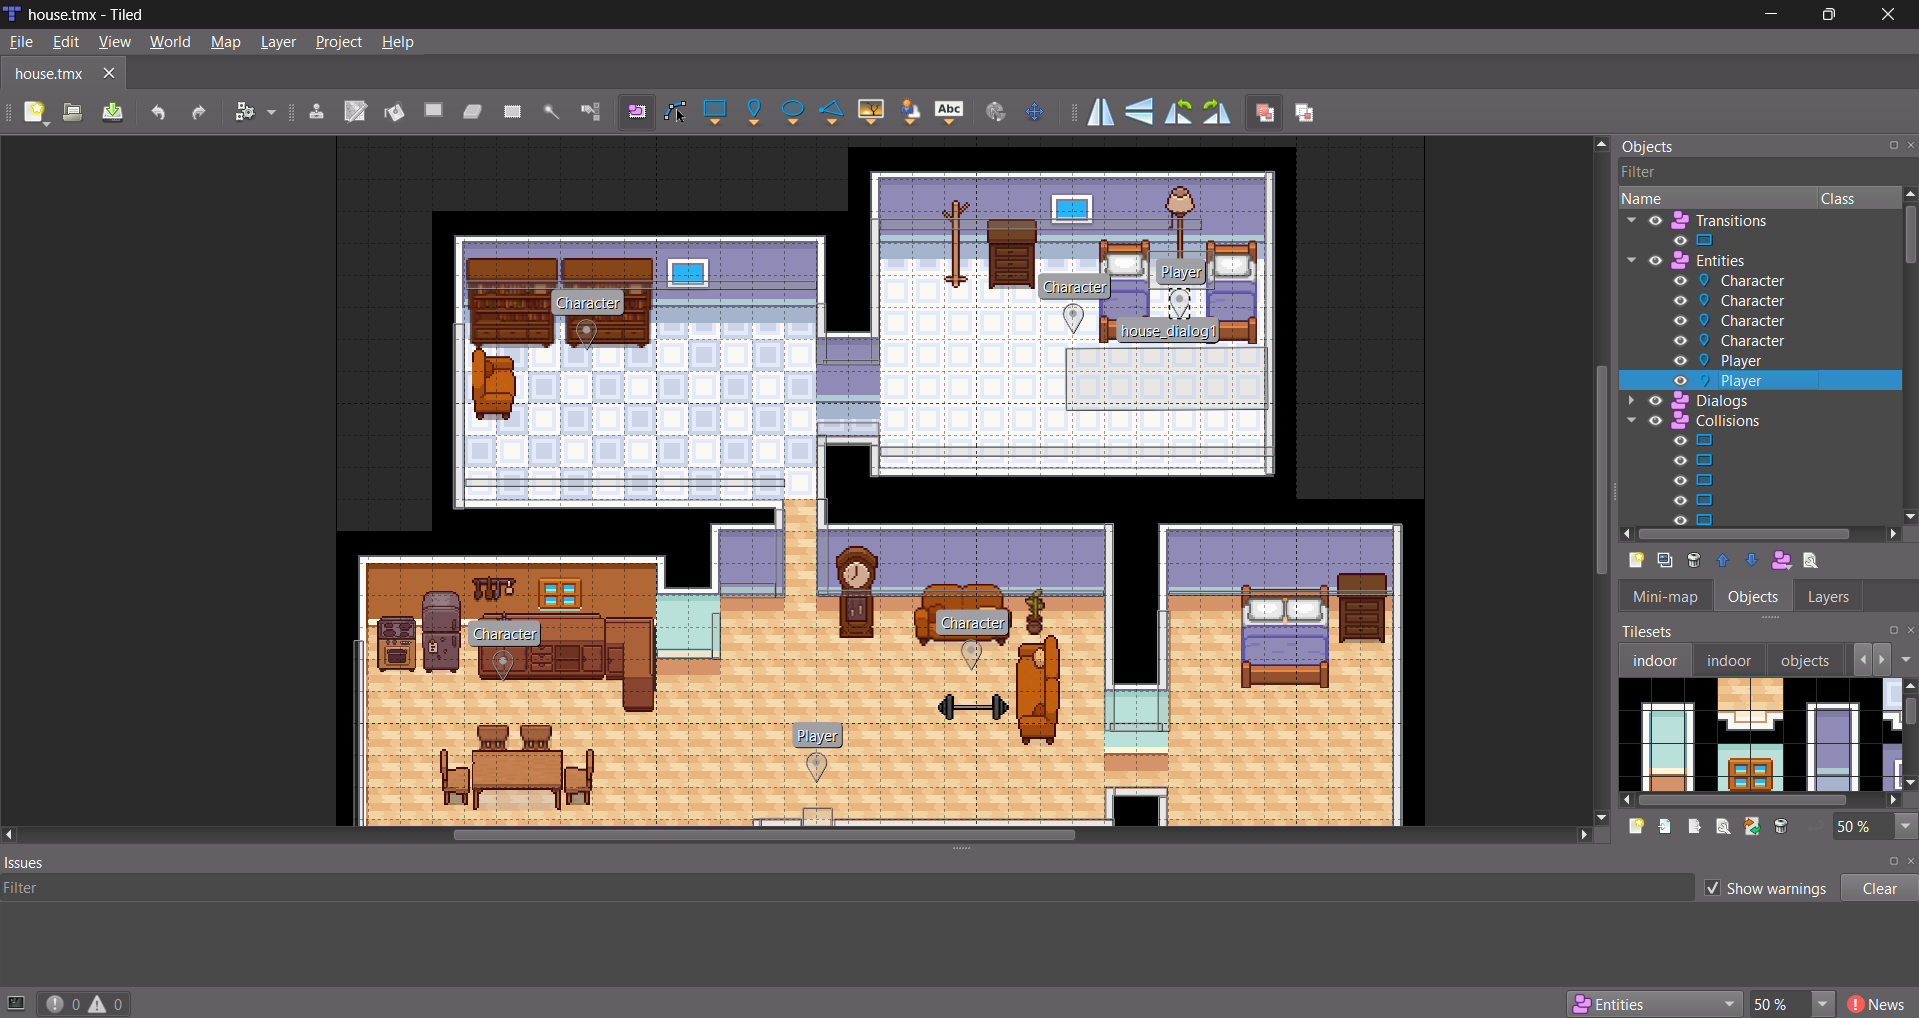
\includegraphics[width=1\linewidth]{figuras/tiled-house.png}
    \caption{Posicionamento de Objetos no Software Tiled }
    \label{fig:tiled-house}
\end{figure}

\begin{figure}[h!]
    \centering
    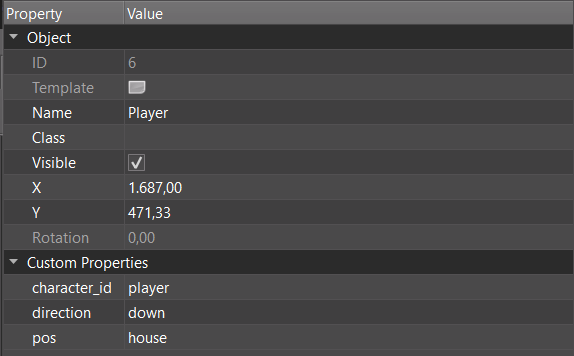
\includegraphics[width=1\linewidth]{figuras/tiled-player-properties.png}
    \caption{Propriedades da Entidade Player no Tiled}
    \label{fig:tiled-player-properties}
\end{figure}

\clearpage
Animação como explicado na seção \ref{sec:animacao} é uma ilusão gerada pela sequência de imagens sendo alternadas a uma determinada velocidade. No Super Labes World para fazer uso dessa técnica é criado um dicionário, sendo a chave o nome do estado em que o jogador se encontra e o valor um vetor de imagens relacionadas aos possíveis estados. A figura mostra a figura a seguir:
\begin{figure}[h!]
    \centering
    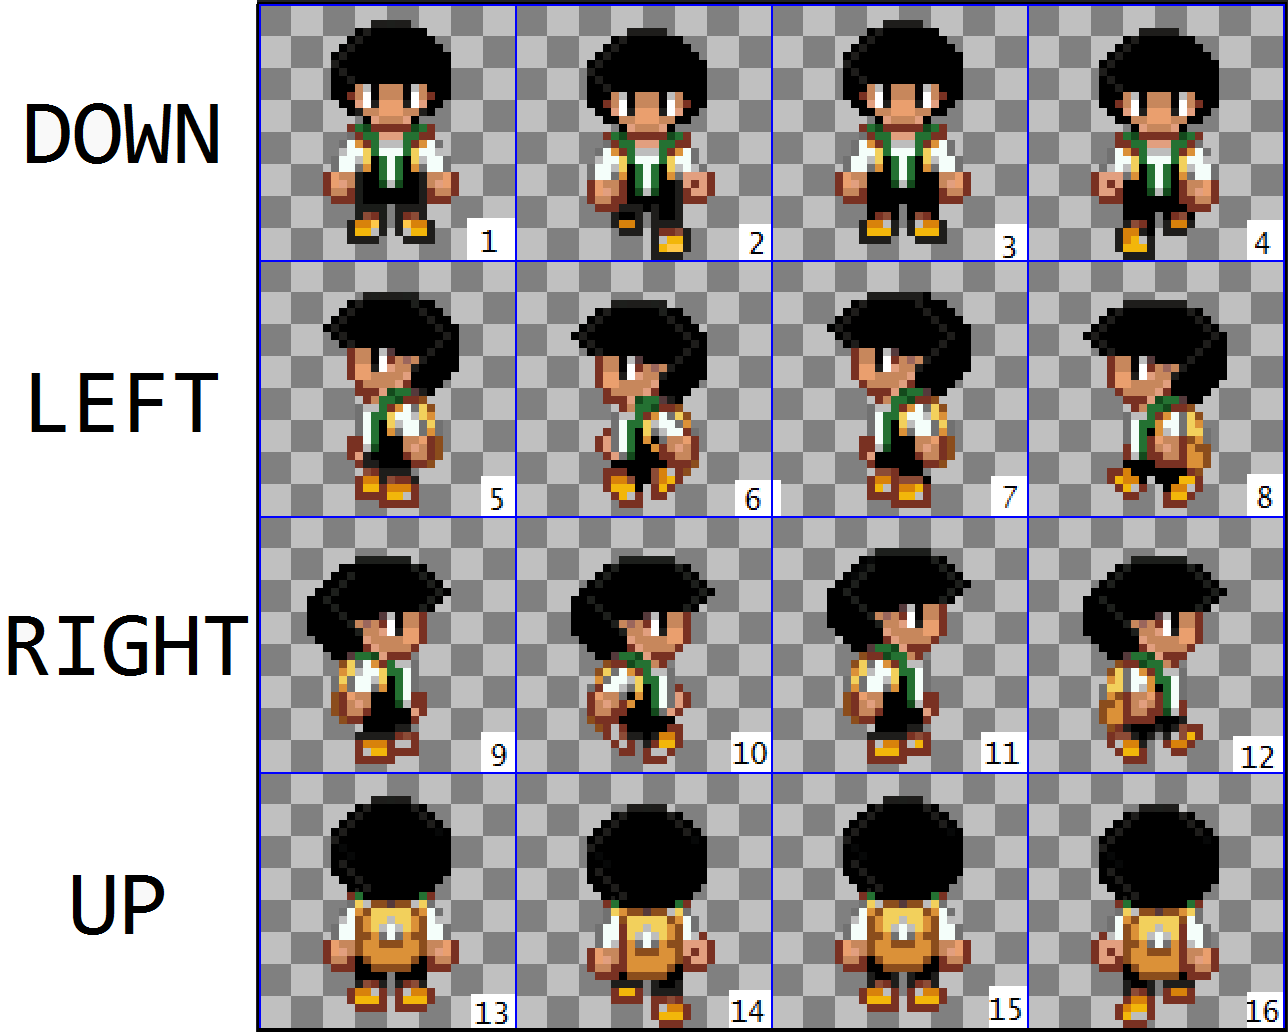
\includegraphics[width=1\linewidth]{figuras/player-animation.png}
    \caption{\textit{Sprite} de Animação do \textit{Player} }
    \label{fig:player-animation}
\end{figure}

Cada chave do dicionário contém quatro imagens (frames), também são criados quatro estados adicionais com o sufixo \textit{''idle''} (parado) correspondente a cada direção. Isso é feito para que quando o jogador pare a movimentação, o programa mude o \textit{frame} para a direção atual do player porém parado. 
\begin{enumerate}
    \item \textit{\textbf{down:}} Mantém as imagens 1, 2, 3 e 4;
    \item \textit{\textbf{down\_idle:}} Mantém a imagem 1;
    \item \textit{\textbf{left:}} Mantém as imagens 5, 6, 7 e 8;
    \item \textit{\textbf{left\_idle:}} Mantém a imagem 5;
    \item \textit{\textbf{right:} Mantém as imagens 9, 10, 11 e 12};
    \item \textit{\textbf{right\_idle:}} Mantém a imagem 9;
    \item \textit{\textbf{up:}} Mantém as imagens 13, 14, 15 e 16 ;
    \item \textit{\textbf{up\_idle:}} Mantém a imagem 13;
\end{enumerate}

% detalhar mais aqui
Para realizar a animação do personagem principal no código foram criados os seguintes métodos.
\lstinputlisting[label=lst-player-animation, caption=Player animation, language=Python, float=htpb]{codigos/player_animation.py}
\begin{itemize}
    \item \textit{\textbf{animate:}} Intercala os frames do personagem de acordo com o retorno da função \textit{get\_state:} enquanto estiver sendo chamada;
    \item \textit{\textbf{get\_state:}} Retorna a direção atual do jogador;
    \item \textit{\textbf{input:}}  Retorna um vetor [x, y] direcional normalizado relativo as teclas que o jogador jogador pressionou;
    \item \textit{\textbf{move:}} Realiza a movimentação do personagem de acordo com o vetor obtido anteriormente;
    \item \textit{\textbf{update:}} Função que é chamada no \textit{loop} principal do jogo, é a partir dela que todas as anteriores são chamadas;

\end{itemize}
% Uma função que fique intercalando os frames de acordo com o estado atual do jogador, uma função que retorne o estado atual do jogador, uma função para capturar a entrada de teclado do jogador e retorne um vetor com a direção, uma função para movimentação e uma função para atualização. Essas funções são descritas a seguir na listagem \ref{lst-player-animation}.

% A função \textit{animate} alterna a imagem do personagem a partir da variável \textit{frame\_index} essa cujo valor vai aumentando conforme o \textit{delta time} e \textit{ANIMATION\_SPEED} que é uma constante usada para definir quão rápido serão as animações do jogo. A função \textit{get\_state} retorna qual estado que o jogador está, que é a chave para o dicionário de frames. A função input a função \textit{move} realiza a movimentação do personagem propriamente dito, e a update é o event loop relativo ao player


Ao carregar o sprite do personagem para o jogo percebe-se que a area relativa ao retangulo é consideravelmente menor do que a área desenhada \ref{fig:player}.
% existe um problema, o retângulo do player é muito maior do que a imagem do personagem,
No Pygame existe um método do Pygame para lidar com isso, o método \textit{inflate}. Essa função diminui o tamanho de um retângulo caso seja passado um valor negativo de parâmetro, e aumenta caso o valor seja positivo. É feito isso e atribuímos a variável \textit{hitbox} essa variável do tipo \textit{Rect} representa a área colidível do jogador. A listagem \ref{lst-player-hitbox} mostra a utilização do método e a figura \ref{fig:player-hitbox} simula o resultado diminuindo a largura pela metade e 60 píxels de altura.

\begin{lstlisting}[language=Python,breaklines, caption= Uso da Função \textit{inflate}, label= lst-player-hitbox]
self.hitbox = self.rect.inflate(-self.rect.width / 2, -60)
\end{lstlisting}
\begin{figure}[h!]
    \centering
    
\includegraphics[width=0.7\linewidth]{figuras/player-hitbox.png}
    \caption{\textit{Hitbox} do personagem principal após o a chamada do método \textit{blit}}
    \label{fig:player-hitbox}
\end{figure}

\section{Game Loop do Super Labes World}
\label{sec:game-loop-super-labes-world}
% game loop
\lstinputlisting[label=lst-game-loop, caption=Main, language=Python, float=htpb]{codigos/game_loop.py}

O game loop é o núcleo principal do jogo, ele é responsável por manter o jogo em execução contínua até que o jogador feche o programa ou o jogo termine. Nele são processados um conjunto tarefas continuamente, no nosso programa, a função é a ilustrada na listagem \ref{lst-game-loop}, o loop e composto pelos seguintes passos.
\begin{enumerate}
    \item Preencher o \textit{background} de preto a área que do mapa que não contém tiles é preenchida com preto (linha 6);
    \item Atualizar o valor do \textit{delta time} (linha 7). Sua importância foi explicada na seção \ref{sec:delta-time};
    \item Verificar o evento de fechar o jogo (linhas 8 a 11);
    \item Chamar a função de \textit{input} que lida com a entrada de controles do jogador (linha 14);
    \item Verificar se o jogador colidiu com um \textit{sprite} de transição (linha 15). Se for o caso então é chamada a função \textit{setup} com os devidos parâmetros do mapa a ser transicionado;
    \item Verificar se o jogador colidiu com alguma caixa de diálogo (linha 16). Se sim então é chamado a função para criar o diálogo com a mensagem;
    \item Atualizar a posição de todos os sprites da tela (linha 17). Essa função chama o método update de todos os sprites contidos no \textit{Group all\_sprites}; 
    \item Desenhar todos os sprites da tela;
    \item Verificar se tem alguma sobreposição do jogo. Existem cinco possíveis sobreposições da tela no jogo, são elas;
        \begin{itemize}
        \item \textit{\textbf{dialog\_open: }} Verdadeiro quando o jogador aperta \textit{spacebar} 
        próximo a uma personagem do jogo, então troca de contexto do \textit{loop} principal para o \textit{loop} da classe \textit{Dialog};
        \item \textit{\textbf{inventory\_open: }}Verdadeiro caso de o jogador aperte a tecla ''i'', troca o contexto do \textit{loop} principal para o \textit{loop} da classe \textit{Inventory}; 
        \item \textit{\textbf{computer\_open: }} Verdadeiro quando o jogador aperta \textit{spacebar} próximo a \textit{InteractiveObject} com o \textit{item\_id} = \textit{computer}. Então troca de contexto do \textit{loop} principal para o \textit{loop} da classe \textit{Computer};
        \item \textit{\textbf{battle\_open: }}  Verdadeiro quando o jogador o jogador responde sim para um desafio de um personagem. Nesse caso troca-se de contexto para a batalha;
        \item \textit{\textbf{choose\_dialog\_open: }} Verdadeiro ao fim de um diálogo de um personagem que contém questões e que não foi derrotado;
    \end{itemize}
\end{enumerate}
% input
A função \textit{input} é a responsável por detectar e lidar com todas as entradas de comandos do jogador, exceto a movimentação do jogador que explicada. Nela são definidas todos os possíveis comandos e controles do jogo. O primeiro passo a ser realizado antes de capturar a entrada do jogador é verificar se o mesmo não está bloqueado. Os bloqueios do jogo são feitos através das sobreposições explicadas anteriormente.  
% Por isso antes de verificar a entrada do jogador é conferido os valores das variáveis \textit{booleanas} \textit{dialog\_open} que se verdadeira o jogador está dialogando, \textit{choose\_dialog\_open} se verdadeiro o jogador está na interface de seleção da resposta e \textit{battle\_open} verdadeira quando o jogador está em uma batalha.
Se o jogador não está bloqueado, então é feita a captura da entrada. Os possíveis controles do jogo são.
\begin{itemize}
    \item \textbf{Tecla I: }Abre o inventário e coloca o player no estado bloqueado;
    \item \textbf{Tecla ESC: }Fecha as interfaces de inventário, computador e tira o jogador do estado bloqueado;
    \item \textbf{Tecla \textit{Spacebar}: }A tecla de interação do jogador, quando pressionada é verificado se o jogador está perto a um personagem, ou a um objeto interativo. Quando for o caso a função leva para o respectivo tratamento;
\end{itemize}

Veja a seguir na listagem \ref{lst-input} o código especificamente.
\lstinputlisting[label=lst-input, caption=Input, language=Python, float=htpb]{codigos/input.py} 

% ==============================================================================
% PG - Nome do Aluno
% Capítulo 4 - Avaliação
% ==============================================================================
\chapter{Apresentação e Avaliação da Proposta}
\label{sec-avaliacao}

% Este capítulo deve ser incluso na monografia quando tiver sido realizado algum tipo de avaliação da proposta que requeira uma descrição detalhada (por exemplo, experimentos, simulações, etc.) O capítulo deve apresentar a avaliação realizada, deixando claro qual foi objetivo da avaliação, os passos realizados, os resultados obtidos e a interpretação desses resultados considerando o objetivo inicial. Em casos em que a avaliação realizada não demande um capítulo dedicado a ela (por ser muito simples ou pequena, por exemplo), ela pode ser tratada em uma seção específica no capítulo anterior.


Este capítulo está dividido em duas partes principais. Na primeira, são apresentadas as telas principais do jogo, desenvolvidas como resultado final do processo de criação. Durante a exibição das telas serão feitos comentários breves sobre o que está sendo mostrado. Na segunda parte serão analisados os resultados da pesquisa que foi realizado através de um formulário. 

\section{Apresentação da Aplicação}
A figura \ref{fig:home-super-labes-world} apresenta a tela inicial ao executar o programa. Nessa tela é possível iniciar um novo jogo, abrir a tela de créditos que contém o link para o repositório do Github com mais informações, abrir a tela de controles do \textit{game}, ou sair do jogo.
\begin{figure}[h!]
    \centering
    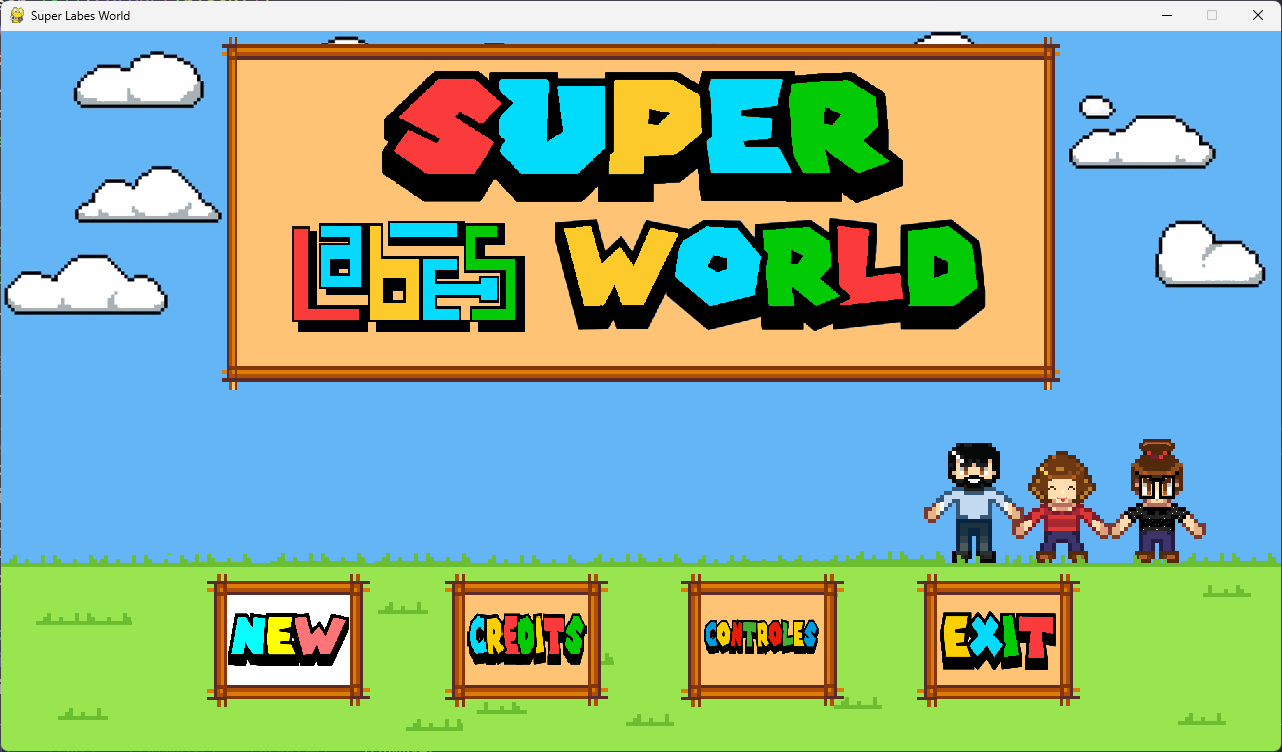
\includegraphics[width=1\linewidth]{figuras/home-super-labes-world.png}
    \caption{Figura ilustrando a home do jogo}
    \label{fig:home-super-labes-world}
\end{figure}

 \newpage
 A próxima tela ilustrada na figura \ref{fig:inventory} mostra como é o \textit{layout} de inventário do jogo. nela é possível ver os items que o jogador carrega e a descrição, o limite do inventário são 30 items. 
\begin{figure}[h!]
    \centering
    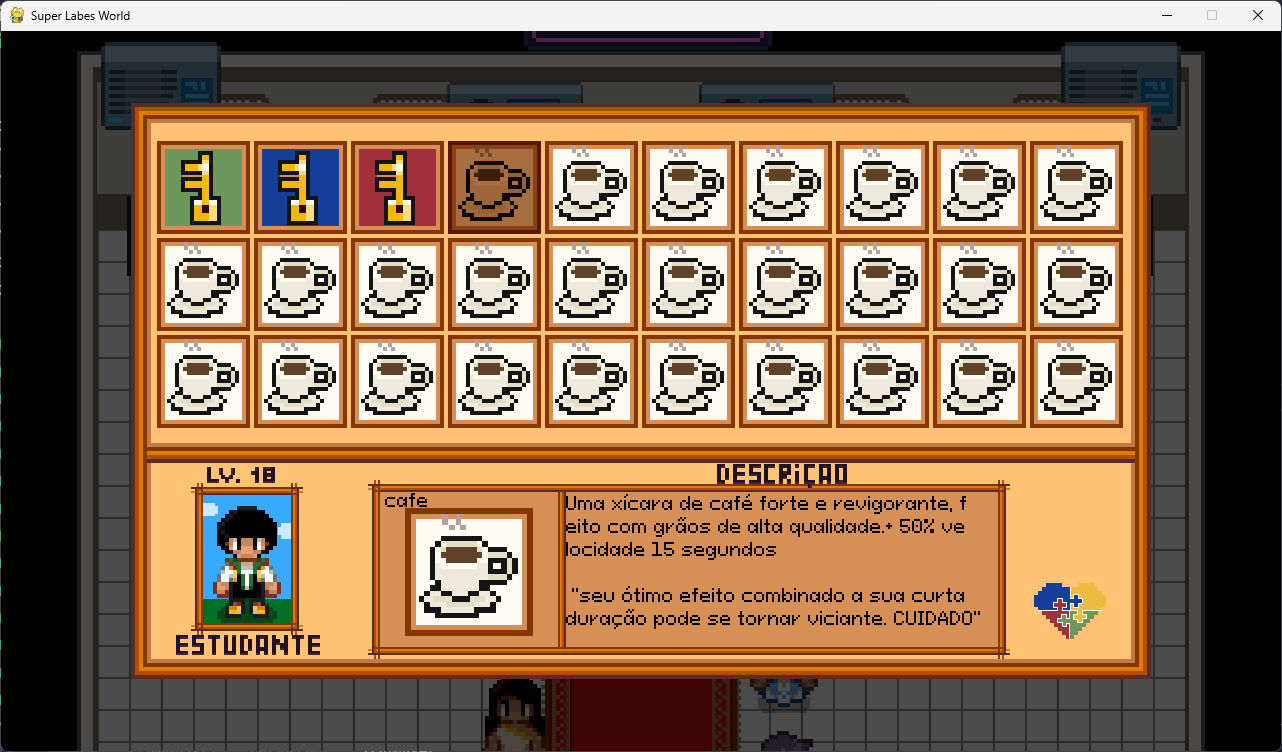
\includegraphics[width=1\linewidth]{figuras/inventory.png}
    \caption{Figura ilustrando o inventário do jogo}
    \label{fig:inventory}
\end{figure}

\clearpage
A figura a seguir \ref{fig:dialog} mostra o jogador interagindo com um dos chefes do jogo antes de entrar em uma batalha.

\begin{figure}[h!]
    \centering
    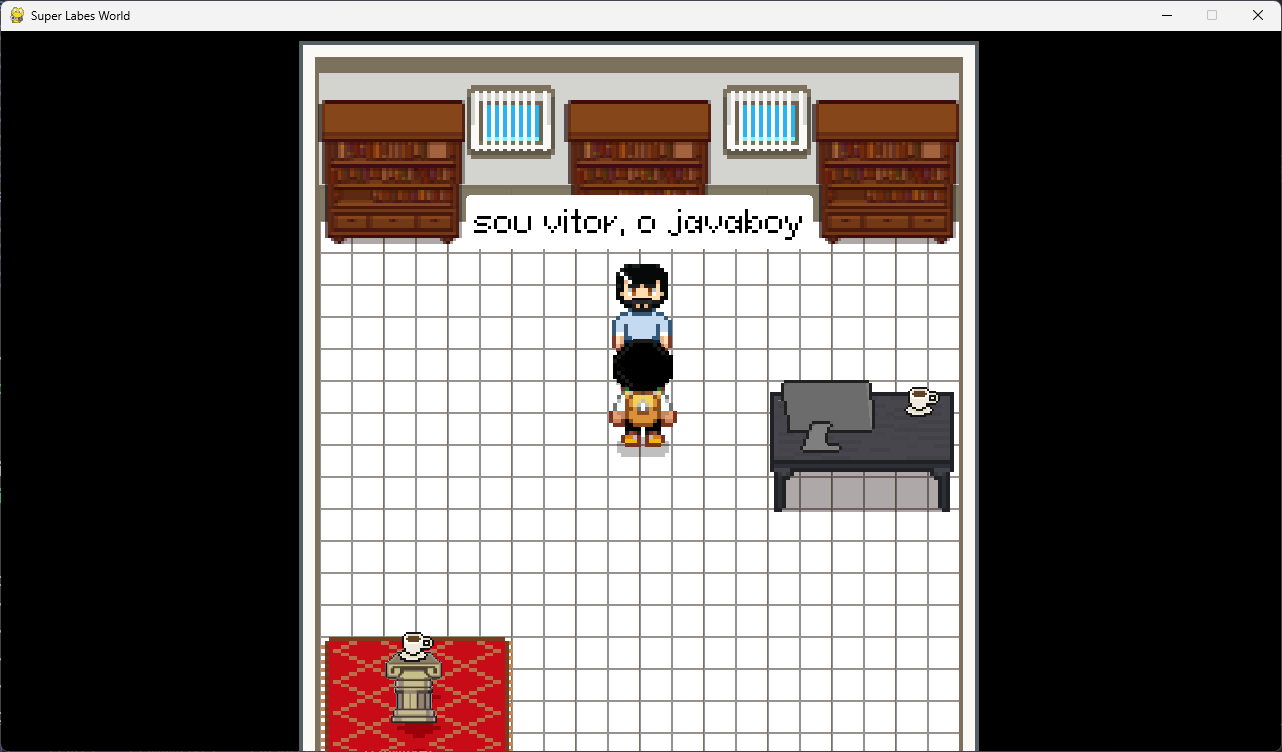
\includegraphics[width=1\linewidth]{figuras/dialog.png}
    \caption{Ilustração de um diálogo do Super Labes World}
    \label{fig:dialog}
\end{figure}
\newpage
Na figura \ref{fig:battle} podemos ver como é a interface da mecânica principal de jogo a batalha de questões. O retângulo superior esquerdo (1) ilustra a pergunta que o jogador tem que responder, o retângulo superior direito (2) mostra o texto dito pelo chefe ao responder a questão, o retângulo intermediário (3) mostra as informações do chefe, os retângulos inferiores vermelho, amarelo, verde e azul (4) são as alternativas a serem escolhidas pelo jogador. Cada opção selecionada altera o texto escrito no retângulo inferior esquerdo de cor branca (5), que é a descrição da resposta. 

\begin{figure}[h!]
    \centering
    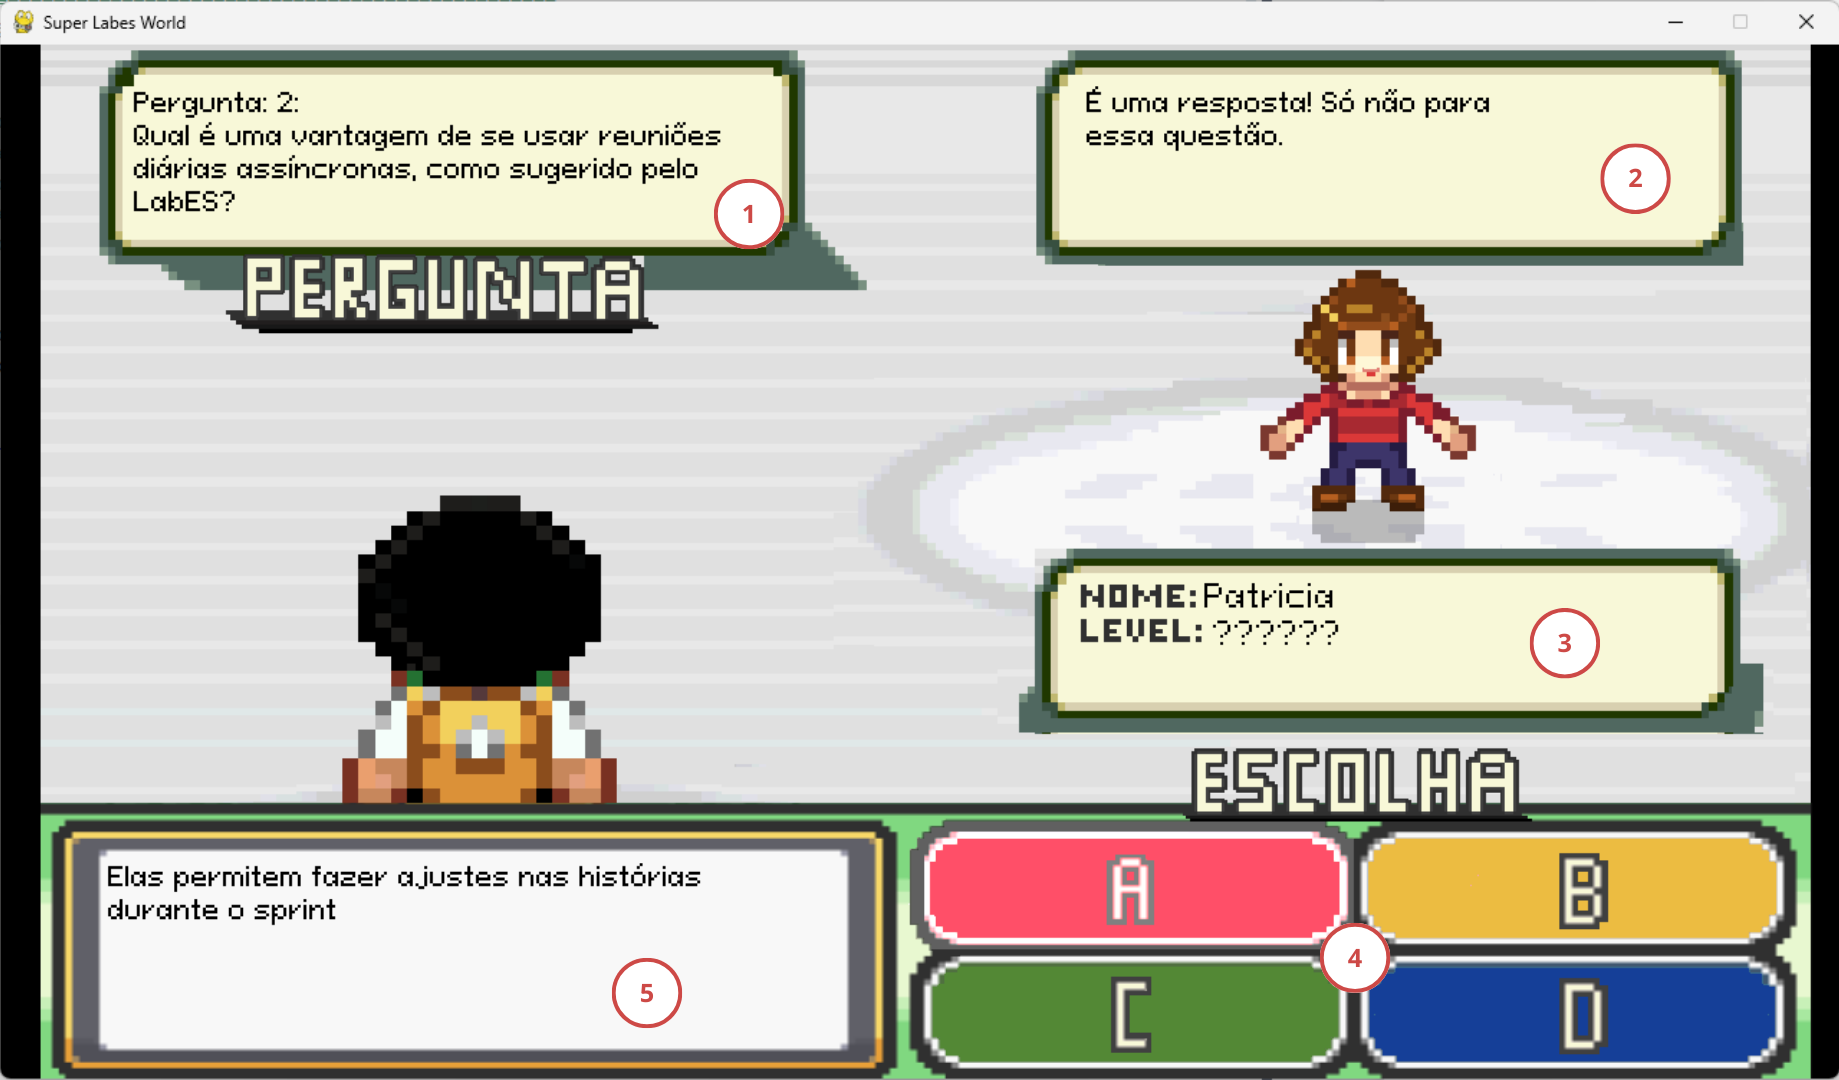
\includegraphics[width=1\linewidth]{figuras/battle.png}
    \caption{Ilustração do sistema de batalha do \textit{game}}
    \label{fig:battle}
\end{figure}
\newpage
Na figura \ref{fig:computer} pode ser vista a interface de computador do jogo, nela é possível o jogador estudar através do jogo. Esse menu contém vários \textit{links} para materiais de estudo que são uteis para vencer o jogo. Caso o jogador abra essa interface após uma batalha com um professor, o computador terá somente os \textit{links} associados as perguntas que o usuário errou.
\begin{figure}
    \centering
    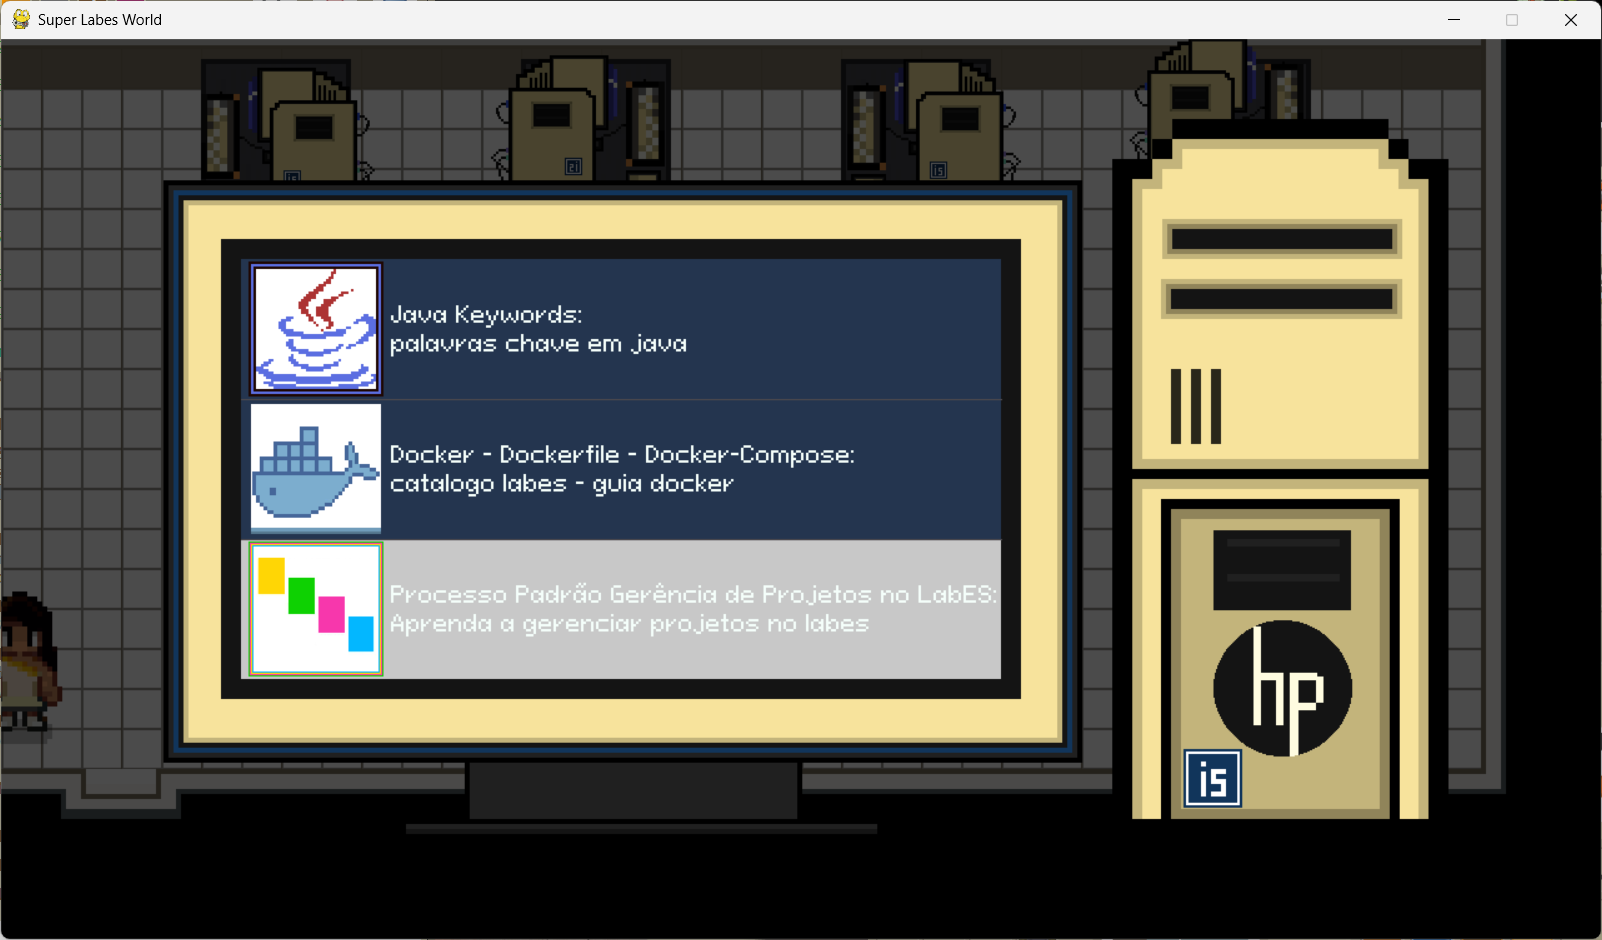
\includegraphics[width=1\linewidth]{figuras/computer.png}
    \caption{\textit{Layout} do computador no jogo usado para acessar \textit{links} de materiais de estudo}
    \label{fig:computer}
\end{figure}

\section{Avaliação do Jogo}
\label{sec:avaliacao-do-jogo}
Com o término do desenvolvimento do jogo, deu-se início à etapa de avaliação e validação do jogo com os principais potenciais usuários desse sistema, os membros do LabES. O objetivo dessa fase foi analisar a jogabilidade em um contexto de uso real, e também obter métricas, com relação aos parâmetros básicos de qualidade de software e dos objetivos propostos pelo jogo. Após os usuários terminarem de jogar, foi-lhes disponibilizado um formulário e tivemos os seguintes resultados.

\begin{figure}[h!]
    \centering
    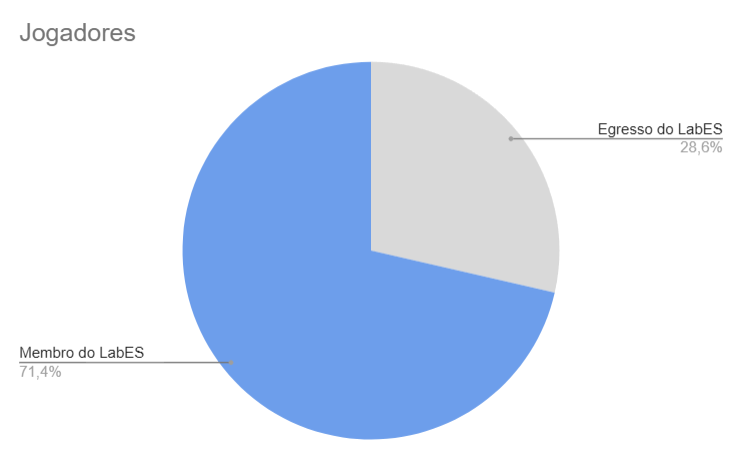
\includegraphics[width=0.8\linewidth]{figuras/players-pizza.png}
    \caption{Percentual de jogadores membros e egressos do LabES que participaram da pesquisa}
    \label{fig:players-pizza}
\end{figure}

A Figura \ref{fig:players-pizza} mostra o percentual dos usuários que jogaram o Super Labes World, a maioria são membros atualmente no LabES. Dentre os que concluíram o jogo, o tempo médio para finaliza-lo foi 35 minutos. O jogo em sua versão atual conta três chefes sendo dois com 10 perguntas, e um com 11, totalizando 31 perguntas de múltipla escolha com quatro alternativas. 

\begin{figure}[h!]
    \centering
    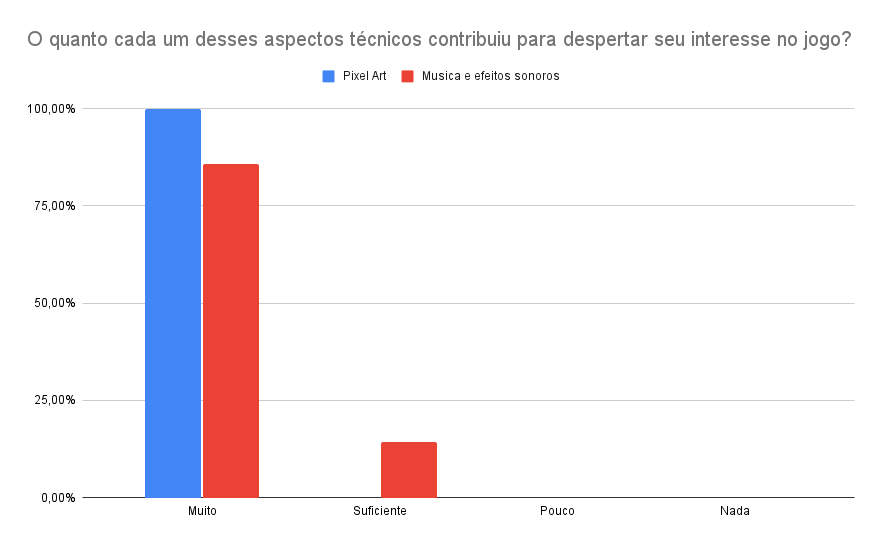
\includegraphics[width=1\linewidth]{figuras/graph-2.png}
    \caption{Gráfico de barras ilustrando os resultados da pesquisa de sobre interesses técnicos no jogo}
    \label{fig:graph-2}
\end{figure}
\clearpage
O uso da \textit{Pixel Art} foi um grande motivador de interesse aos usuários, 100\% dos jogadores responderam que esse aspecto foi relevante para o seu engajamento no jogo. Quanto a trilha sonora foi importante para 85\% desses mesmos usuários.

\begin{figure}[h!]
    \centering
    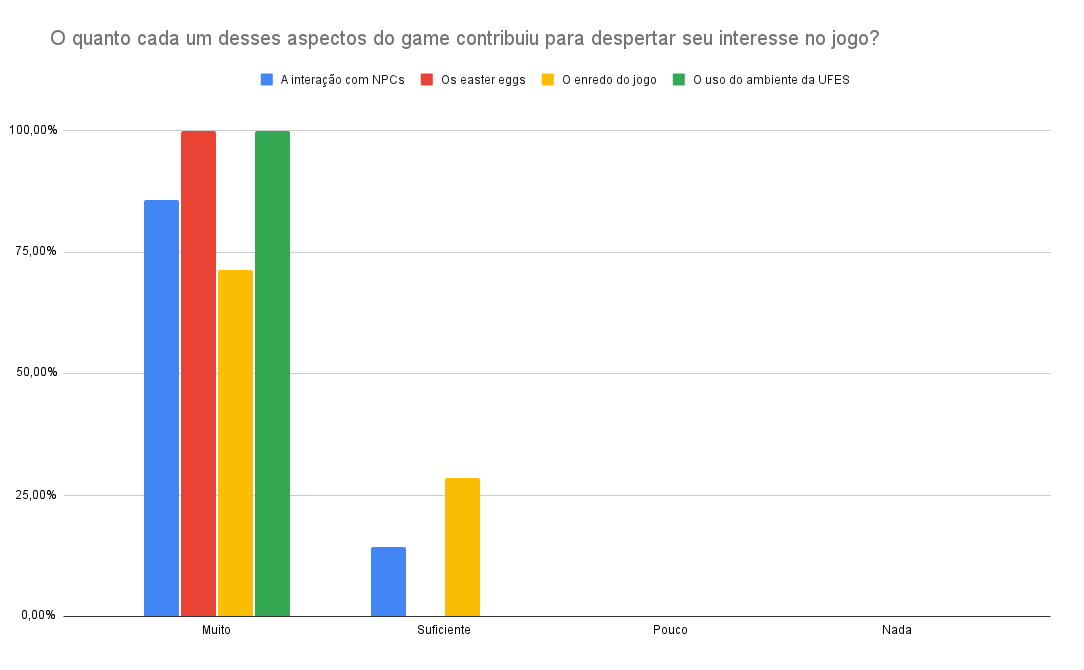
\includegraphics[width=1\linewidth]{figuras/graph-3.png}
    \caption{Gráfico de barras ilustrando os resultados da pesquisa de sobre aspectos do jogo}
    \label{fig:graph-3}
\end{figure}

Os \textit{easter eggs} (segredos de caráter humorísticos), e a ambientação do jogo se passar na UFES também foram unânimes em aceitação entre os jogadores. A figura \ref{fig:graph-3} mostra o resultado da pesquisa em relação a aspectos do \textit{game} que despertaram o interesse. 

\clearpage
A avaliação geral de todos os jogadores sobre o jogo ficou com uma média 4.71 de 5, no geral a maioria teve uma experiencia positiva e agradável com ao jogar o Super Labes World. Todos os entrevistados responderam sim para a pergunta: ''você acredita que video-game é uma boa forma de aprendizado?'' e  '' O Super Labes World o estimulou a aprender?''. Essas foram perguntas chave para motivação desse trabalho. 

A tabela \ref{tbl-relatos-jogo} mostra alguns depoimentos de jogadores que concluíram o jogo.
\begin{table}[h!]
	\caption{Tabela com alguns relatos sobre a seguinte pergunta '' Você acredita que o jogo foi uma boa forma de aprendizado? ''.}
	\label{tbl-relatos-jogo}
	\centering
	\renewcommand{\arraystretch}{2}
	\begin{small}
		\begin{tabular}{ | p{35mm} | p{100mm} |}\hline
			  % \centering{\textbf{Classe}} & \textbf{Descrição}  \\\hline
			\centering{Pessoa 1} & ''Às vezes, quando estamos muito atarefados com as coisas da faculdade, a vontade de aprender não é suficiente. A proposta de um jogo pode ser boa para um aprendizado mais tranquilo e atrativo e que não dê a sensação de "peso" que estudo pra provas às vezes podem dar.'' \\\hline
			\centering{Pessoa 2} & ''É uma boa forma de aprender coisas simples, que muitas vezes as pessoas que já estão no projeto E podem acabar esquecendo se ensinar.'' \\\hline
			\centering{Pessoa 3} & ''Realmente me forçou a pesquisar sobre e ler as recomendações para avançar no jogo.'' \\\hline
                \centering{Pessoa 4} & ''O jogo cria objetivos mais palpáveis e de curto prazo com recompensas instantâneas facilitando o senso de progressão e estimulando o estudo sobre o tema do jogo.'' \\\hline
		\end{tabular}
	\end{small}
\end{table}

Por fim a pergunta fundamental e que foi a principal motivadora para o desenvolvimento desse trabalho foi sobre foi respondida na figura 

\begin{figure}[h!]
    \centering
    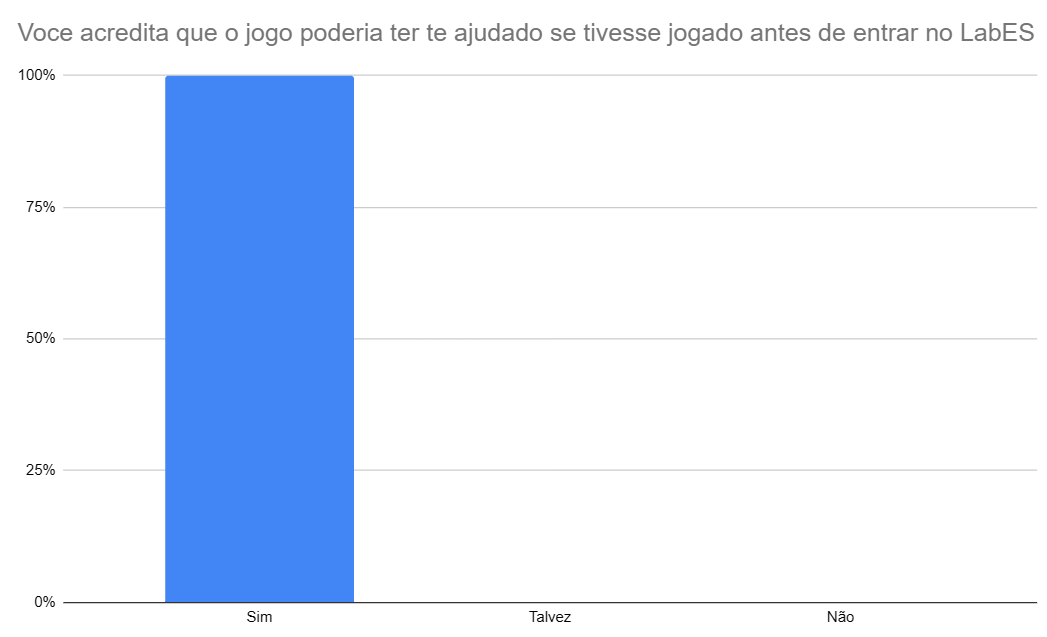
\includegraphics[width=0.81\linewidth]{figuras/graph-1.png}
    \caption{Gráfico de barras ilustrando o resultado para a pergunta motivadora para desenvolvimento do jogo}
    \label{fig:graph-1}
\end{figure}
% ==============================================================================
% PG - Nome do Aluno
% Capítulo 5 - Considerações Finais
% ==============================================================================
\chapter{Conclusão}
\label{sec-conclusoes}


% Neste capítulo devem ser realizadas as considerações finais do trabalho, sendo apresentadas suas principais contribuições, limitações, lições aprendidas durante o desenvolvimento do trabalho, dificuldades enfrentadas e perspectivas de trabalhos futuros. O capítulo deve ter entre 3 e 5 páginas.


%%% Início de seção. %%%
\section{Considerações Finais}
\label{sec-conclusoes-consideracoes}

% Esta seção deve apresentar um texto de fechamento do trabalho, devendo incluir considerações sobre o trabalho desenvolvido, suas limitações, contribuições, experiência adquirida pelo aluno e lições aprendidas ao longo do desenvolvimento, bem como dificuldades enfrentadas durante o desenvolvimento do trabalho. Nesta seção é preciso mostrar claramente a relação entre os resultados produzidos no trabalho e os objetivos estabelecidos no Capítulo~\ref{sec-intro} 

Neste projeto de graduação, foi desenvolvido o jogo \textit{Super Labes World}, cujo objetivo é auxiliar os novos integrantes do LabES a compreenderem, ou revisarem caso já saibam assuntos pertinentes ao LabES, afim de melhorar sua integração nos projetos. O jogo apresenta essa proposta de maneira interativa e lúdica, proporcionando uma experiência didática descontraída. No jogo o jogador interpreta um aluno da UFES que tem como objetivo entrar no SigAMAES, um dos projetos do LabES. O objetivo do jogo é vencer os desafios propostos pelos professores e adquirir as três chaves, essas chaves são uma prova de que o aluno possui aquele conhecimento. Ao jogador conseguir todas essas chaves o jogador pode então ter acesso ao LabES.



% Apesar do foco do jogo ser os membros do LabES nessa versão, o jogo pode facilmente ser continuado e adaptado para diferentes contextos e áreas da UFES. O código do jogo está disponível publicamente junto com essa monografia que pode ser utilizada como referencial para programadores e \textit{game designers}. 

Este trabalho de conclusão de curso também pode ser relevante para interessados e entusiastas na área de \textit{game design}, uma vez que essa monografia apresentou e detalhou tecnologias, ferramentas e a metodologia usada no desenvolvimento de jogo. Esses conceitos podem ser aplicados a diferentes jogos. O código fonte do jogo está disponível publicamente junto com essa monografia no Github.

O uso das bibliotecas Pygame e Pytmx permitiram abstrair várias camadas de abstração proporcionando um desenvolvimento eficiente e ágil do jogo. Os softwares Tiled e Aseprite também cumpriram um papel importante para a criação desse \textit{game}, o uso de suas documentações foram essenciais para rápido entendimento das ferramentas. Foi possível aplicar boas práticas de programação e de engenharia de software, aprendidas durante a graduação, que resultaram num código altamente flexível e aberto à alterações e expansões.

Reavaliando os objetivos dessa monografia, descritos na seção \ref{sec-intro}, consideramos que foram integralmente alcançados. Os resultados alcançados com a finalização do jogo foram extremamente positivos nesse contexto, o uso de jogos para educação se mostrou uma ferramenta com alto potencial de ensino e . Isso pode ser comprovado na seção \ref{}

Pensando nas dificuldades enfrentadas durante o processo de criação do jogo, a primeira a ser superada foi a curva de aprendizado . É comum ao desenvolver algo novo enfrentar dificuldades, ter que aprender novas ferramentas, bibliotecas, \textit{frameworks}, mas, com base sólida que o foi adquirida durante o curso foi possível vencer. A segunda foi o tempo, o desenvolvimento de um jogo exige diversas competências interdisciplinares. No mercado, profissionais especializados são contratados para cuidar de cada aspecto do jogo, como falado na seção \ref{sec-desenvolvimento-de-jogos}, mesclar todas essas habilidades neste trabalho foi um desafio.

Com uma ideia inicialmente enorme e as dificuldades citadas no parágrafo anterior para com o desenvolvimento do jogo, os conhecimentos obtidos ao longo do curso foram fundamentais. A busca por ''dividir e conquistar'' os problemas que surgiram no caminho foi a estratégia utilizada e com resultados.

Finalmente, entendemos que esse projeto final de graduação foi bem-sucedido.

%%% Início de seção. %%%
\section{Trabalhos Futuros}
\label{sec-conclusoes-trabalhosfuturos}

% Nesta seção devem ser identificados trabalhos futuros que poderão ser realizados a partir dos resultados obtidos até o momento no trabalho. Idealmente, trabalhos futuros não devem apenas ser citados. Recomenda-se discutir aspectos sobre como podem ser realizados e por que é importante que sejam realizados (que benefícios podem ser obtidos com sua realização).

O \textit{Super Labes World} apresenta grande potencial para crescimento e expansão, visto que é um jogo do gênero RPG e sua ambientação não foi totalmente explorada. O jogo possui três professores e consequentemente três batalhas, porém, é possível adicionar novos personagens e consequentemente novas batalhas. Algumas ideias que surgiram durante o processo de desenvolvimento do jogo foram.

\begin{itemize}
    \item Um sistema de moedas, onde o jogador ganha recompensas ao vencer batalhas que poderão serem trocadas por recompensas em outros mapas, por exemplo na cantina;
    \item Novos mapas, muitos locais da UFES poderiam ser adicionados;
    \item Novos personagens, o acréscimo de novos personagens seria necessária;
    \item Um sistema de customização de personagem ao iniciar o jogo;
    \item Adição de um mini-mapa, indicando o jogador áreas que não foram exploradas;
    \item Desenvolvimento de um sistema de \textit{save game}, para que o jogador não precise terminar o jogo de uma vez;
    \item Novos items;
    \item Novos materiais de estudo;
    \item O sistema de adição de perguntas aos personagens poderia ser através de planilhas, para facilitar a alteração de questões para todos os tipos de usuários;
    \item Novas mecânicas de jogo;
    \item Tornar o Super Labes World em um MMO \textit{(Massively Multiplayer Online)} ou seja multijogadores massivos online;

\end{itemize}
% % ==============================================================================
% % PG - Nome do Aluno
% % Capítulo 6 - Dicas LaTeX
% % ==============================================================================
% \chapter{Dicas para escrita em \latex}
% \label{sec-dicaslatex}

% Utilizaremos este capítulo para apresentar alguns exemplos de uso de \latex que podem ser úteis para aqueles que possuem pouca experiência com a ferramenta e vão escrever a monografia usando \latex. Para mais informações sobre \latex, você pode consultar a  \href{https://www.overleaf.com/learn}{documentação do overleaf} ou vários materiais disponíveis online, como  \href{https://www.ime.usp.br/~viviane/MAP2212/minicurso.pdf}{esse minicurso da USP}.

% Este capítulo deve ser excluído da monografia. Sugere-se também excluir as figuras e listagens usadas aqui como exemplo.



% %%% Início de seção. %%%
% \section{Seções e subseções}
% \label{sec-dicaslatex-secoes}

% O documento é organizado em capítulos (\texttt{\textbackslash chapter\{\}}), seções (\texttt{\textbackslash section\{\}}), subseções (\texttt{\textbackslash subsection\{\}}), sub-subseções (\texttt{\textbackslash subsubsection\{\}}) e assim por diante. Atenção, porém, a não criar estruturas muito profundas (sub-sub-sub-...) pois o documento não fica bem estruturado.


% %%% Início de seção. %%%
% \subsection{Referências a seções}
% \label{sec-dicaslatex-secoes-refs}

% Cada parte do documento (capítulo, seção, etc.) deve possuir um rótulo logo abaixo de sua definição. Por exemplo, este capítulo é definido com \texttt{\textbackslash chapter\{Introdução\}} seguido por \texttt{\textbackslash label\{sec-dicaslatex\}}. Assim, podemos fazer referências cruzadas usando o comando \texttt{\textbackslash ref\{rótulo\}}: ``O Capítulo~\ref{sec-dicaslatex} começa com a Seção~\ref{sec-dicaslatex-secoes}, que é ainda subdividida nas subseções~\ref{sec-dicaslatex-secoes-refs} e~\ref{sec-dicaslatex-secoes-sobrerefs}.

% Para melhor organização das partes do documento, sugere-se primeiro utilizar o prefixo \texttt{sec-} (para diferenciar de referências à figuras, tabelas, etc. quando usarmos o comando \texttt{\textbackslash ref\{\}}) e também representar a hierarquia das seções nos rótulos. Por exemplo, o Capítulo~\ref{sec-dicaslatex} tem rótulo \texttt{sec-dicaslatex}, sua Seção~\ref{sec-dicaslatex-secoes} tem rótulo \texttt{sec-dicaslatex-secoes} e a Subseção~\ref{sec-dicaslatex-secoes-refs} tem rótulo \texttt{sec-dicaslatex-secoes-refs}.



% %%% Início de seção. %%%
% \subsection{Sobre referências cruzadas}
% \label{sec-dicaslatex-secoes-sobrerefs}

% Nas próximas seções, veremos que é possível fazer referência cruzada não só a seções mas também a listagens de código, figuras, tabelas, etc. Em todos estes casos, quando nos referimos à Seção X, Listagem Y ou Figura Z, consideramos que estes são os nomes próprios destes elementos e, portanto, usa-se a primeira letra maiúscula. Isso pode ser visto na Subseção~\ref{sec-dicaslatex-secoes-refs}, acima. A exceção é quando nos referimos a vários elementos ao mesmo tempo, por exemplo: ``as subseções~\ref{sec-dicaslatex-secoes-refs} e~\ref{sec-dicaslatex-secoes-sobrerefs}''.

% Por fim, ao usar o comando \texttt{\textbackslash ref\{\}}, sugere-se separá-lo da palavra que vem antes dele com um \textasciitilde\ ao invés de espaço. Por exemplo: \texttt{o capítulo\textasciitilde \textbackslash ref\{sec-dicaslatex\}}. Isso faz com que o \latex não quebre linha entre a palavra \texttt{capítulo} e o número do capítulo.




% %%% Início de seção. %%%
% \section{Citações bibliográficas}
% \label{sec-dicaslatex-citacoes}

% Este documento utiliza a ferramenta de gerenciamento de referências bibliográficas do \latex, chamada \emph{BibTeX}. O arquivo \texttt{bibliografia.bib}, referenciado no arquivo \latex principal deste documento, contém algumas referências bibliográficas de exemplo. Assim como capítulos, seções, etc., tais referências também possuem rótulos, especificados como primeiro parâmetro de cada entrada (ex.: \texttt{@incollection\{souza-et-al:iism08, ...\}}.

% Sugere-se um padrão para rótulos de referências bibliográficas para que fique claro também no código \latex qual referência está sendo citada. Por exemplo, ao citar a referência \texttt{souza-et-al:sesas13}, sabemos que é um artigo escrito por \emph{Souza} e outros, publicado no \emph{SESAS} em \emph{2013} (geralmente a pessoa que citou sabe que publicação é SESAS e quem é Souza).

% Para citar uma referência bibliográfica contida no arquivo \emph{BibTeX}, basta usar seu rótulo como parâmetro de um de dois comandos possíveis de citação:

% \begin{itemize}
% 	\item O comando \texttt{\textbackslash cite\{\}} efetua uma citação tradicional, colocando o nome do(s) autor(es) e o ano entre parênteses. Por exemplo, \texttt{\textbackslash cite\{souza-et-al:iism08\}} é transformado em \cite{souza-et-al:iism08};
	
% 	\item O comando \texttt{\textbackslash citeonline\{\}} efetua uma citação integrada ao texto, colocando o nome do(s) autor(es) direto no texto e somente o ano entre parênteses. Por exemplo, ``de acordo com \texttt{\textbackslash citeonline\{souza-et-al:iism08\}}'' é transformado em: de acordo com \citeonline{souza-et-al:iism08};
% \end{itemize}

% Também é possível citar vários trabalhos de uma só vez, separando os rótulos das referências bibliográficas com uma vírgula dentro do comando apropriado. Por exemplo, \texttt{\textbackslash cite\{souza-et-al:sesas13,souza-et-al:csrd13\}} \cite{souza-et-al:sesas13,souza-et-al:csrd13}.

% Os trabalhos citados são automaticamente incluídos na seção de referências bibliográficas, ao final do documento. Tudo é formatado automaticamente segundo padrões da ABNT.



% %%% Início de seção. %%%
% \section{Listagens de código}
% \label{sec-dicaslatex-listagens}

% O pacote \texttt{listings}, incluído neste template, permite a inclusão de listagens de código. Análogo ao já feito anteriormente, listagens possuem rótulos para que possam ser referenciadas e sugerimos uma regra de nomenclatura para tais rótulos: usar como prefixo o rótulo do capítulo, substituindo \texttt{sec-} por \texttt{lst-}.

% A Listagem~\ref{lst-intro-exemplo}, por exemplo, possui o rótulo \texttt{lst-intro-exemplo} e representa o código que foi usado no próprio documento para exibir as listagens desta seção. Como podemos ver, a sugestão é que os arquivos de código sejam colocados dentro da pasta \texttt{codigos/} e tenham nome idêntico ao rótulo, colocando a extensão adequada ao tipo de código.

% \lstinputlisting[label=lst-intro-exemplo, caption=Exemplo de código \latex para inclusão de listagens de código., float=htpb]{codigos/lst-intro-exemplo.tex}

% A Listagem~\ref{lst-intro-outroexemplo} mostra um exemplo de listagem com especificação da linguagem utilizada no código. O pacote \texttt{listings} reconhece algumas linguagens\footnote{Veja a lista de linguagens suportadas em \url{http://en.wikibooks.org/wiki/LaTeX/Source\_Code\_Listings\#Supported_languages}.} e faz ``coloração'' de código (na verdade, usa \textbf{negrito} e não cores) de acordo com a linguagem. O parâmetro \texttt{float=htpb} incluído em ambos os exemplos impede que a listagem seja quebrada em diferentes páginas.

% \lstinputlisting[label=lst-intro-outroexemplo, caption=Exemplo de código \java especificando linguagem utilizada., language=Java, float=htpb]{codigos/lst-intro-outroexemplo.java}



% %%% Início de seção. %%%
% \section{Figuras}
% \label{sec-dicaslatex-figuras}

% Figuras podem ser inseridas no documento usando o \emph{ambiente} \texttt{figure} (ou seja, \texttt{\textbackslash begin\{figure\}} e \texttt{\textbackslash end\{figure\}}) e o comando \texttt{\textbackslash includegraphics\{\}}. Existem alguns outros elementos e propriedades úteis de serem configuradas, resultando no código exibido na Listagem~\ref{lst-intro-figuras}.

% \lstinputlisting[label=lst-intro-figuras, caption=Código \latex utilizado para inclusão das figuras na Seção~\ref{sec-dicaslatex-figuras}., float=htpb]{codigos/lst-intro-figuras.tex}

% O comando \texttt{\textbackslash centering} centraliza a figura na página. A opção \texttt{width} do comando \texttt{\textbackslash includegraphics\{\}} determina o tamanho da figura e usa-se \texttt{\textbackslash textwidth} (opcionalmente multiplicado por um número) para se referir à largura da página.

% O parâmetro do comando \texttt{\textbackslash includegraphics\{\}} indica onde a imagem pode ser encontrada. Foi criado o diretório \texttt{figuras/} para conter as figuras do documento, dando uma melhor organização aos arquivos. Ao abrir esta pasta, repare que as figuras possuem duas versões---uma em \texttt{.eps} e outra em \texttt{.pdf}---e que o comando \texttt{\textbackslash includegraphics\{\}} não especifica a extensão. Isso se dá porque o \latex possui um compilador para formato PostScript (\texttt{latex}) que espera as imagens em \texttt{.eps} e um compilador para PDF (\texttt{pdflatex}) que espera as imagens em \texttt{.pdf}. Dependendo do seu ambiente \latex, é possível apenas colocar as figuras em formatos mais comuns, como JPG ou PNG e ele incluir no PDF sem problemas. Vale a pena testar.

% Por fim, o comando \texttt{\textbackslash caption\{\}} especifica a descrição da figura e \texttt{\textbackslash label\{\}}, como de costume, estabelece um rótulo para permitir referência cruzada de figuras. Note ainda que é utilizada a mesma estratégia de nomenclatura de rótulos usada nas listagens, porém utilizando o prefixo \texttt{fig-}.

% As figuras~\ref{fig-intro-exemplo} e~\ref{fig-intro-exemplosideways} mostram o resultado do código da Listagem~\ref{lst-intro-figuras}. A Figura~\ref{fig-intro-exemplosideways}, em particular, utiliza o pacote \texttt{rotating} para mostrar figuras largas em modo paisagem. Basta usar o ambiente \texttt{sidewaysfigure} ao invés de \texttt{figure}.

% \begin{figure}
% 	\centering
% 	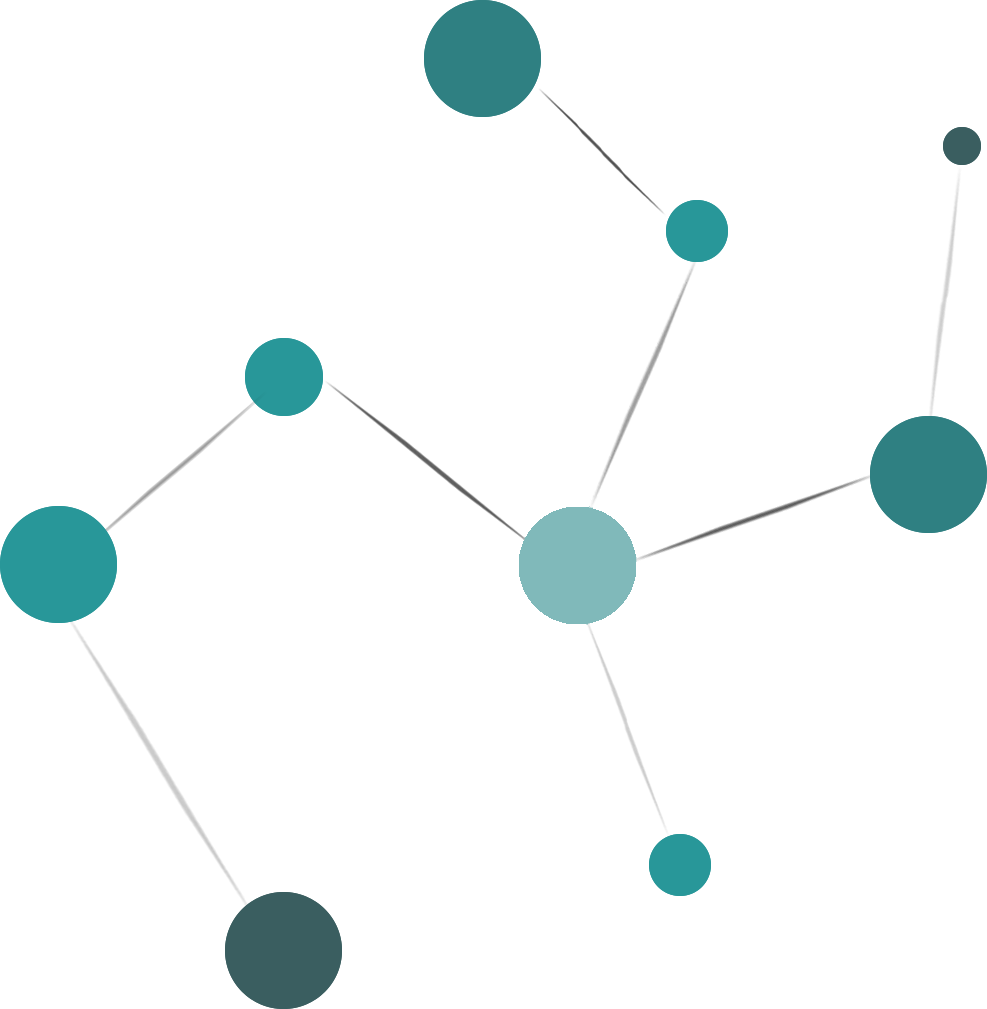
\includegraphics[width=.25\textwidth]{figuras/image-home.png} 
% 	\caption{Exemplo de figura.}
% 	\label{fig-intro-exemplo}
% \end{figure}

% \begin{sidewaysfigure}
% 	\centering
% 	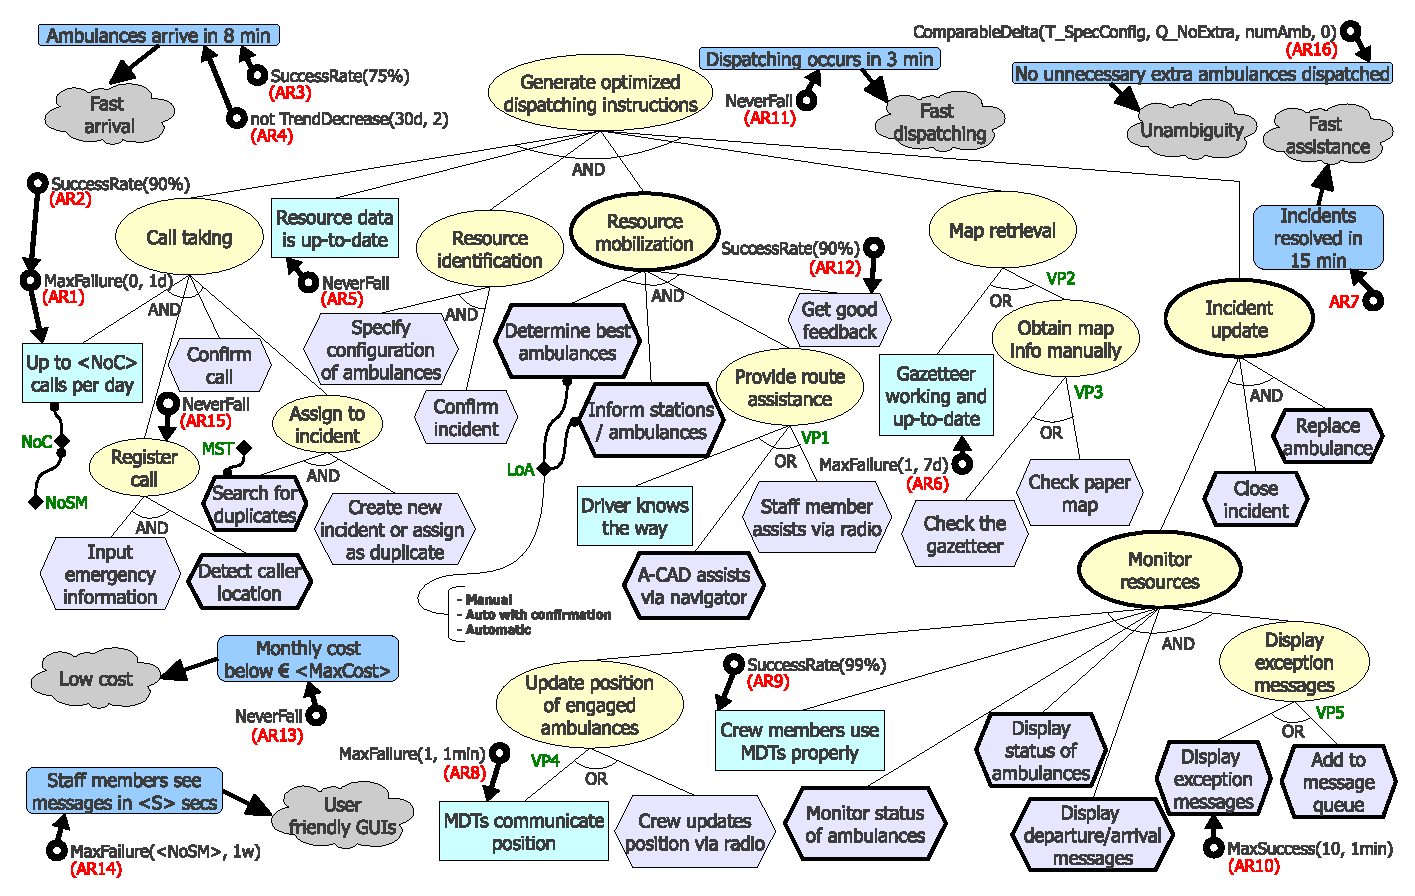
\includegraphics[width=\textwidth]{figuras/fig-intro-exemplosideways} 
% 	\caption{Exemplo de figura em modo paisagem: um modelo de objetivos~\cite{souza-mylopoulos:spe13}.}
% 	\label{fig-intro-exemplosideways}
% \end{sidewaysfigure}



% %%% Início de seção. %%%
% \section{Tabelas}
% \label{sec-dicaslatex-tabelas}

% Tabelas são um ponto fraco do \latex. Elas são complicadas de fazer e, dependendo da complexidade da tabela (muitas células mescladas, por exemplo), vale a pena construi-las em outro programa (por exemplo, em seu editor de texto favorito) e inclui-las no documento como figuras. Mostramos, no entanto, alguns exemplos de tabela a seguir. O código utilizado para criar as tabelas encontra-se nas listagens~\ref{lst-intro-tabelas01}, \ref{lst-intro-tabelas02} e~\ref{lst-intro-tabelas03}.

% \lstinputlisting[label=lst-intro-tabelas01, caption=Código \latex utilizado para inclusão das tabelas~\ref{tbl-intro-exemplo01} e~\ref{tbl-intro-exemplo02}., float=htpb]{codigos/lst-intro-tabelas01.tex}

% \lstinputlisting[label=lst-intro-tabelas02, caption=Código \latex utilizado para inclusão da Tabela~\ref{tbl-intro-exemplo03}., float=htpb]{codigos/lst-intro-tabelas02.tex}

% \lstinputlisting[label=lst-intro-tabelas03, caption=Código \latex utilizado para inclusão da Tabela~\ref{tbl-intro-exemplo04}., float=htpb]{codigos/lst-intro-tabelas03.tex}

% Em particular, a Tabela~\ref{tbl-intro-exemplo04} utiliza um pacote chamado \texttt{tabularx}, que permite maior controle do layout das tabelas. Ao definir o ambiente \texttt{\textbackslash begin\{tabularx\}}, são definidos os tamanhos de cada coluna proporcional à largura ocupada pela tabela. Veja na Listagem~\ref{lst-intro-tabelas03} que as primeiras duas colunas não definem o atributo \texttt{\textbackslash hsize}, o que faz com que elas fiquem com o tamanho padrão de coluna, que é a largura da tabela dividida pelo número de colunas. Já a terceira coluna define \texttt{\textbackslash hsize=1.2\textbackslash hsize}, ou seja, esta coluna deve ser 20\% maior do que o tamanho padrão. Para isso, é preciso retirar de outras colunas, portanto a quarta e quinta colunas são definidas como 10\% menores (ou seja, \texttt{\textbackslash hsize=0.9\textbackslash hsize}).

% % Exemplo de tabela 01:
% \begin{table}
% 	\caption{Exemplo de tabela com diferentes alinhamentos de conteúdo.}
% 	\label{tbl-intro-exemplo01}
% 	\centering
% 	\begin{tabular}{ | c | l | r | p{40mm} |}\hline
% 		\textbf{Centralizado} & \textbf{Esquerda} & \textbf{Direita} & \textbf{Parágrafo}\\\hline
% 		C & L & R & Alinhamento de tipo parágrafo especifica largura da coluna e quebra o texto automaticamente.\\
% 		\hline
% 		Linha 2 & Linha 2 & Linha 2 & Linha 2\\
% 		\hline
% 	\end{tabular}
% \end{table}

% % Exemplo de tabela 02:
% \begin{table}
% 	\caption{Exemplo que especifica largura de coluna e usa lista enumerada (adaptada de~\cite{souza-mylopoulos:spe13}).}
% 	\label{tbl-intro-exemplo02}
% 	\centering
% 	\renewcommand{\arraystretch}{1.2}
% 	\begin{small}
% 		\begin{tabular}{ | p{15mm} | p{77mm} | p{55mm} |}\hline
% 			\textbf{\textit{AwReq}} & \textbf{Adaptation strategies} & \textbf{Applicability conditions}\\\hline
			
% 			AR1 &
% 			\vspace{-2mm}\begin{enumerate}[topsep=0cm, partopsep=0cm, itemsep=0cm, parsep=0cm, leftmargin=0.5cm]
% 				\item \textit{Warning(``AS Management'')}
% 				\item \textit{Reconfigure($\varnothing$)}
% 			\end{enumerate}\vspace{-4mm} &
% 			\vspace{-2mm}\begin{enumerate}[topsep=0cm, partopsep=0cm, itemsep=0cm, parsep=0cm, leftmargin=0.5cm]
% 				\item Once per adaptation session;
% 				\item Always.
% 			\end{enumerate}\vspace{-4mm}
% 			\\\hline
			
% 			AR2 &
% 			\vspace{-2mm}\begin{enumerate}[topsep=0cm, partopsep=0cm, itemsep=0cm, parsep=0cm, leftmargin=0.5cm]
% 				\item \textit{Warning(``AS Management'')}
% 				\item \textit{Reconfigure($\varnothing$)}
% 			\end{enumerate}\vspace{-4mm} &
% 			\vspace{-2mm}\begin{enumerate}[topsep=0cm, partopsep=0cm, itemsep=0cm, parsep=0cm, leftmargin=0.5cm]
% 				\item Once per adaptation session;
% 				\item Always.
% 			\end{enumerate}\vspace{-4mm}
% 			\\\hline
% 		\end{tabular}
% 	\end{small}
% \end{table}

% % Exemplo de tabela 03:
% \begin{table}
% 	\caption{Exemplo que mostra equações em duas colunas (adaptada de~\cite{souza-mylopoulos:spe13}).}
% 	\label{tbl-intro-exemplo03}
% 	\centering
% 	\vspace{1mm}
% 	\fbox{\begin{minipage}{.98\linewidth}
% 			\begin{minipage}{0.51\linewidth}
% 				\vspace{-4mm}
% 				\begin{eqnarray}
% 				\Delta \left( I_{AR1} / NoSM \right) \left[ 0, maxSM \right] > 0\\
% 				\Delta \left( I_{AR2} / NoSM \right) \left[ 0, maxSM \right] > 0\\
% 				\Delta \left( I_{AR3} / LoA \right) < 0\\
% 				\end{eqnarray}
% 				\vspace{-6mm}
% 			\end{minipage}
% 			\hspace{2mm}
% 			\vline 
% 			\begin{minipage}{0.41\linewidth}
% 				\vspace{-4mm}
% 				\begin{eqnarray}
% 				\Delta \left( I_{AR11} / VP2 \right) < 0\\
% 				\Delta \left( I_{AR12} / VP2 \right) > 0\\
% 				\Delta \left( I_{AR6} / VP3 \right) > 0\\
% 				\end{eqnarray}
% 				\vspace{-6mm}
% 			\end{minipage}
% 	\end{minipage}}
% \end{table}

% % Exemplo de tabela 04:
% \begin{table}[h]
% 	\caption{Exemplo que utiliza o pacote \texttt{tabularx}, extraído de um artigo ainda não publicado.}
% 	\label{tbl-intro-exemplo04}
% 	\centering\tiny\def\tabularxcolumn#1{m{#1}}
% 	\begin{tabularx}{\columnwidth}{ >{\centering}X | >{\centering}X | >{\hsize=1.2\hsize\centering}X | >{\hsize=0.9\hsize\centering}X | >{\hsize=0.9\hsize\centering\arraybackslash}X }
% 		\hline
% 		\textbf{Applied Criteria} & \textbf{Analyzed Content} & \textbf{Initial\\Occurrences} & \textbf{Final Results} & \textbf{Reduction (\%)} \\
% 		\hline
% 		Duplicate Removal & Title, authors and year & 903 & 420 & 54,84\% \\ 
% 		\hline 
% 		IC and ECs & Title, abstract and keywords & 420 & 130 & 69,05\% \\ 
% 		\hline 
% 		IC and ECs & Full text & 130 & 117 & 10\% \\ 
% 		\hline 
% 		Final Results & -- & 903 & 117 & 87,04\% \\ 
% 		\hline 
% 	\end{tabularx}
% \end{table}



%%% Páginas finais do documento: bibliografia e anexos. %%%

% Finaliza a parte no bookmark do PDF para que se inicie o bookmark na raiz e adiciona espaço de parte no sumário.
\phantompart

% Marca o início dos elementos pós-textuais.
\postextual

% Referências bibliográficas
\bibliography{bibliografia}


% Apêndices.
\begin{apendicesenv}

% Imprime uma página indicando o início dos apêndices.
\partapendices

% (*) Incluir como apêndice a documentação técnica produzida durante o PG (especificação de requisitos,
% projeto arquitetural, etc.). Utilizar o exemplo \includepdf caso o documento seja produzido em outro
% editor de texto (Microsoft Word, LibreOffice Writer) e transformado em PDF. Utilizar o exemplo \include
% caso os documentos tenham sido também escritos em LaTeX.
% \includepdf[pages={1-}]{apendices/apendice01-requisitos.pdf}
% \includepdf[pages={1-}]{apendices/apendice02-projeto.pdf}
% \include{ap1-requisitos}
% \include{ap2-projeto}
\end{apendicesenv}


% Índice remissivo.
\phantompart
\printindex

% Fim do documento.
\end{document}
